\documentclass[10pt,a4paper,twocolumn]{article}

\usepackage[utf8]{inputenc}
\usepackage[T1]{fontenc}
\usepackage{mathptmx}
\usepackage{amsmath,amssymb,amsfonts,amsthm}
\usepackage{mathrsfs}
\usepackage{graphicx}
\usepackage{booktabs}
\usepackage{tabularx}
\usepackage{array}
\usepackage{xcolor}
\usepackage{fancyhdr}
\usepackage{geometry}
\usepackage{caption}
\usepackage{cite}
\usepackage[colorlinks=true,linkcolor=darkblue,citecolor=darkblue,urlcolor=darkblue]{hyperref}

\geometry{
  a4paper,
  left=14mm,
  right=14mm,
  top=16.5mm,
  bottom=18.5mm,
  headheight=12pt,
  headsep=6.5mm,
  footskip=8.5mm,
  columnsep=6.5mm
}

\definecolor{darkblue}{RGB}{20, 55, 110}
\definecolor{boxbg}{RGB}{242, 246, 252}
\definecolor{boxframe}{RGB}{30, 75, 140}

\pagestyle{fancy}
\fancyhf{}
\fancyhead[L]{\footnotesize\textit{G. Gautam and R. Kumar: Financial Fraud Detection with Adaptive Self-Attention Fusion (ASAF-GFD)}}
\fancyhead[R]{\footnotesize\textit{Preprint Submitted to Elsevier / IEEE}}
\fancyfoot[L]{\footnotesize\textit{Department of CSE (AI \& ML), DAVIET Jalandhar}}
\fancyfoot[R]{\footnotesize\textbf{Page \thepage\ of 18}}
\renewcommand{\headrulewidth}{0.4pt}
\renewcommand{\footrulewidth}{0.4pt}

\captionsetup{font=small,labelfont=bf,labelsep=colon}

\newtheorem{theorem}{Theorem}
\newtheorem{proposition}{Proposition}

\setlength{\parskip}{0pt}
\makeatletter
\def\@listi{\leftmargin\leftmargini \parsep 0pt \topsep 2.5pt plus 1pt minus 1pt \itemsep 2pt plus 1pt minus 0.5pt}
\let\@listI\@listi
\makeatother
\setlength{\parindent}{1em}
\setlength{\emergencystretch}{3em}
\hbadness=10000
\vbadness=10000
\hfuzz=1pt

\begin{document}

\twocolumn[{%
  \begin{center}
    \vspace*{2pt}
    \noindent\rule{\textwidth}{1.2pt}
    \vspace{8pt}

    {\LARGE\bfseries\color{darkblue} Graph-Based Financial Fraud Detection with Dual-Path\\[3pt]
    Spectral-Spatial Filtering, Adaptive Self-Attention Fusion, and Ant\\[3pt]
    Colony Metaheuristic Optimization (ASAF-GFD)\par}

    \vspace{9pt}
    {\large\bfseries Geetansh Gautam$^{a,\ast}$ and Dr.\ Rajeev Kumar$^{a}$\par}
    \vspace{5pt}
    {\small\itshape $^{a}$Department of Computer Science and Engineering (Artificial Intelligence \& Machine Learning),\\
    DAV Institute of Engineering and Technology (DAVIET), Kabir Nagar, Jalandhar, Punjab 144008, India\par}
    \vspace{3pt}
    {\footnotesize Geetansh Gautam is a B.Tech CSE (AI \& ML) Research Scholar, and Dr.\ Rajeev Kumar is an Assistant Professor in the Department of Computer Science and Engineering (Artificial Intelligence \& Machine Learning), DAV Institute of Engineering and Technology (DAVIET), Jalandhar.\\[2pt]
    $^{\ast}$Corresponding author. E-mail: \texttt{geetanshgautam429@gmail.com} (G. Gautam).\par}
    \vspace{8pt}
    \noindent\rule{\textwidth}{0.6pt}
  \end{center}

  \vspace{2pt}
  \noindent
  \begin{minipage}[t]{0.23\textwidth}
    {\normalsize\bfseries\color{darkblue} A R T I C L E \ \ I N F O}\\[4pt]
    \rule{\linewidth}{0.4pt}\\[6pt]
    {\footnotesize
    \textbf{Keywords:}\\
    Graph Neural Network (GNN)\\
    Spectral Graph Filtering\\
    Beta Wavelet Operator\\
    Heterophily \& Camouflage\\
    Adaptive Self-Attention Fusion\\
    Ant Colony Optimization (ACO)\\
    XGBoost Ensemble\\
    Financial Fraud Detection\\[8pt]
    \textbf{MSC / ACM Classification:}\\
    68T07, 68R10, 91G45\\[8pt]
    \textbf{Code \& Reproducibility:}\\
    Implemented in PyTorch 2.1.1,\\
    DGL 2.2.1, and XGBoost.
    }
  \end{minipage}%
  \hfill
  \begin{minipage}[t]{0.74\textwidth}
    {\normalsize\bfseries\color{darkblue} A B S T R A C T}\\[4pt]
    \rule{\linewidth}{0.4pt}\\[6pt]
    {\small
    Financial fraud detection on large-scale relational transaction networks is a critical yet formidable challenge in modern digital economies. While Graph Neural Networks (GNNs) naturally capture topological dependencies via neighborhood message passing, real-world financial graphs simultaneously exhibit three severe structural pathologies: \textit{relation camouflage}, \textit{high heterophily}, and \textit{extreme class imbalance}. Recent dual-path graph filtering frameworks such as DPF-GFD decouple high-frequency structural anomaly extraction on the original graph from low-pass feature consistency smoothing on a $k$-Nearest Neighbor ($k$NN) similarity graph. However, existing dual-path methods rely on static feature concatenation ($Z = [Z_{1i} \parallel Z_{2i}]$), implicitly enforcing a rigid, uniform 50\%--50\% structural-to-feature importance assumption across every node in the network. In practice, a deeply camouflaged fraudster exhibits strong high-frequency spectral energy in the original graph, whereas a benign account relies heavily on local feature homophily in the $k$NN view. To resolve this fundamental limitation, we propose \textbf{Adaptive Self-Attention Fusion for Graph-Based Fraud Detection (ASAF-GFD)}, a novel frequency-complementary GNN framework calibrated via \textbf{Ant Colony Optimization (ACO)}. ASAF-GFD introduces a learnable, node-specific self-attention gating mechanism enhanced with an inductive/unsupervised structural anomaly energy prior and a residual sigmoid context calibration gate. For each node $v_i$, ASAF-GFD dynamically computes attention weights $(\alpha_{1i}, \alpha_{2i})$ satisfying $\alpha_{1i} + \alpha_{2i} = 1$, amplifying structural anomaly embeddings ($Z_{1i}$) for suspicious nodes while prioritizing $k$NN feature-consistency embeddings ($Z_{2i}$) for benign nodes. Furthermore, we formulate an ACO soft-computing metaheuristic to jointly optimize spectral filter orders, $k$NN neighborhood sizes, attention regularization coefficients, and dual-stage XGBoost ensemble parameters. Extensive experiments over five independent seeds across four real-world financial benchmarks---\textbf{FDCompCN, FFSD, Elliptic, and T-Finance}---demonstrate that ASAF-GFD achieves a 100\% win rate across all 16 dataset-metric pairs ($\text{Rec}@K$, F1, AUC, and AP), including a \textbf{+12.52\% absolute (+44.60\% relative) AP gain} on FDCompCN (0.4059 vs.\ 0.2807) and an AUC of \textbf{0.9808} on Elliptic.
    }
  \end{minipage}
  \vspace{8pt}
  \noindent\rule{\textwidth}{1.0pt}
  \vspace{10pt}
}]

\section{Introduction}

In recent years, the global digital economy has experienced unprecedented expansion, driven by the pervasive integration of cloud banking, instant mobile payment rails, decentralized cryptocurrency ledgers, and automated corporate supply-chain financing. Concurrently, financial cybercrime has evolved from isolated, opportunistic thefts into highly coordinated, adversarial operations orchestrated by transnational fraud syndicates \cite{ref1}. Financial fraud not only inflicts hundreds of billions of dollars in direct monetary losses on consumers, commercial banks, and regulatory institutions annually, but also erodes public trust in digital financial infrastructure and threatens macroeconomic stability \cite{ref2}. Modern financial fraud spans a diverse taxonomy of illicit behaviors, including corporate financial statement falsification \cite{ref41}, credit card transaction laundering \cite{ref42}, illicit cryptocurrency mixing and ransomware payouts \cite{ref43}, and organized synthetic-identity lending default rings \cite{ref44}. As rule-based compliance filters and point-anomaly detectors have matured, adversaries have abandoned standalone fraudulent transactions in favor of complex, multi-hop relational networks designed to obscure illicit capital flows.

Currently, enterprise financial anti-fraud systems confront two overarching operational hurdles. First, the entities participating in modern financial ecosystems---such as bank accounts, corporate suppliers, payment terminals, IP addresses, and hardware devices---are densely interconnected through multi-relational business logic. The anomalous footprints of sophisticated fraudsters are rarely observable from isolated tabular transaction attributes alone; instead, they manifest as subtle topological irregularities embedded within multi-hop interaction subgraphs. Second, adversarial actors continuously adapt their evasion tactics. Ranging from phishing rings and synthetic identity fabrication to automated account takeovers and transaction smurfing, fraudsters actively manipulate both their behavioral attributes and their network connectivity to mimic legitimate financial activity. This non-stationary, adversarial behavior causes conventional risk control models to suffer severe performance degradation in production environments \cite{ref3}.

Early financial fraud detection pipelines relied predominantly on domain-expert rule engines \cite{ref4} and classical statistical machine learning classifiers \cite{ref5}. While symbolic rule sets and threshold triggers offer straightforward auditability for compliance officers, they are inherently passive defenses that suffer from rigid decision boundaries, high false-positive rates, and an inability to generalize to unseen fraud topologies \cite{ref15,ref16}. Traditional supervised learning models---such as Na\"{\i}ve Bayes \cite{ref19}, Support Vector Machines (SVMs) \cite{ref20,ref22}, Random Forests \cite{ref21}, Logistic Regression \cite{ref23}, and gradient-boosted decision trees \cite{ref39}---automated pattern discovery over tabular indicators but remained fundamentally blind to inter-entity relational dependencies. Deep learning architectures, including Multi-Layer Perceptrons (MLPs) \cite{ref24}, Convolutional Neural Networks (CNNs) \cite{ref25,ref26}, and Gated Recurrent Units (GRUs) \cite{ref27}, further reduced reliance on manual feature engineering by extracting hierarchical nonlinear representations from raw transaction logs \cite{ref6}. Nevertheless, because Euclidean deep networks process transactions as independent or purely sequential records, they fail to capture the structural graph topology that binds collusive fraud rings together.

In response to these limitations, Graph Neural Networks (GNNs) \cite{ref7} have emerged as the premier computational paradigm for relational fraud detection. By formulating financial ecosystems as attributed graphs $G = (V, E, X)$ and iteratively propagating information along edges via neighborhood message passing, GNNs jointly encode node attributes and network topology. Specialized fraud detectors such as CARE-GNN \cite{ref8}, ASA-GNN \cite{ref10}, GCD-GNN \cite{ref11}, PC-GNN \cite{ref48}, PMP \cite{ref49}, and CAFD \cite{ref12} have demonstrated substantial gains across credit card, corporate accounting, and cryptocurrency benchmarks. Despite this progress, deploying GNNs on real-world financial graphs exposes three deeply intertwined structural challenges:

\begin{enumerate}
  \item \textbf{Relation Camouflage:} Unlike benign users who naturally interact with peers sharing similar financial profiles, intelligent fraudsters deliberately establish dense transaction or ownership links with numerous legitimate entities while concealing direct ties to accomplices \cite{ref8,ref36}. During standard neighborhood aggregation, features from overwhelming benign neighbors wash out the suspicious signals of camouflaged fraudsters.
  \item \textbf{High Heterophily and Spectral Low-Pass Bias:} Classical spatial GNNs (e.g., GCN \cite{ref45}, GraphSAGE \cite{ref46}, GAT \cite{ref47}) operate under the homophily assumption, where connected nodes share identical class labels. From the perspective of spectral graph theory \cite{ref13,ref33}, standard message passing acts as a spectral low-pass filter that smooths node signals across edges. In heterophilous fraud graphs---where fraudulent nodes preferentially connect to benign targets---low-pass smoothing suppresses high-frequency spectral irregularities that carry the most discriminative anomaly cues \cite{ref32,ref50}.
  \item \textbf{Severe Class Imbalance:} Genuine transactions typically outnumber fraudulent instances by orders of magnitude (often $10:1$ to $100:1$ or higher) \cite{ref38,ref44}. Under extreme label skew, end-to-end neural classifiers experience gradient domination by majority-class samples, resulting in unstable decision boundaries and poor precision-recall trade-offs.
\end{enumerate}

To reconcile spectral anomaly amplification with structural camouflage removal, He et al.\ \cite{ref9} recently introduced the \textbf{Dual-Path Graph Filtering (DPF-GFD)} framework. Rather than relying on single-graph propagation, DPF-GFD decouples fraud representation learning into two complementary branches: (i) a \textit{structural anomaly path} that applies a Beta wavelet-based band-pass filter bank \cite{ref32} to the original transaction graph $\mathscr{G}_1$ to capture multi-frequency structural irregularities, and (ii) a \textit{feature consistency path} that constructs a topology-independent $k$-Nearest Neighbor ($k$NN) similarity graph $\mathscr{G}_2$ in feature space and applies a low-pass filter to restore local homophily among semantically similar nodes. The embeddings from both branches are subsequently concatenated and classified using XGBoost \cite{ref39}.

\vspace{2pt}
\noindent\colorbox{boxbg}{%
  \parbox{\dimexpr\linewidth-2\fboxsep\relax}{%
    \vspace{3pt}
    \textbf{\color{darkblue}Key Research Gap in Existing Dual-Path GNNs:} While DPF-GFD \cite{ref9} successfully decouples spectral anomaly extraction ($Z_1$) from $k$NN feature smoothing ($Z_2$), it fuses the two views via \textbf{static vector concatenation} $Z = [Z_{1i} \parallel Z_{2i}]$. As explicitly acknowledged in the limitations and future work of He et al.\ \cite{ref9}, static concatenation treats both graph paths as uniformly weighted across every node in the network. In real-world financial graphs, however, the relative informativeness of structural vs.\ feature-space signals varies drastically at the individual node level.
    \vspace{3pt}
  }%
}
\vspace{2pt}

Specifically, consider two contrasting nodes in a financial network: (a) a \textit{deeply camouflaged corporate fraudster} whose financial ratios are carefully doctored to resemble average industry peers, but whose multi-hop supplier-shareholder links exhibit sharp high-frequency structural anomalies in $\mathscr{G}_1$; and (b) a \textit{legitimate high-volume enterprise} whose transaction topology spans diverse counterparties, but whose intrinsic accounting features align tightly with benign peers in the $k$NN similarity graph $\mathscr{G}_2$. Under static concatenation $[Z_{1i} \parallel Z_{2i}]$, the noisy $k$NN neighborhood of the camouflaged fraudster dilutes its high-frequency structural alarm, while the irregular topological degree of the benign enterprise contaminates its smooth feature consistency. Furthermore, existing dual-path frameworks rely on naive random search for hyperparameter selection \cite{ref9}, failing to navigate the coupled, non-convex interactions between spectral wavelet order $C$, $k$NN neighborhood size $k$, attention regularization, and tree-ensemble complexity.

To address these foundational gaps, this paper proposes \textbf{Adaptive Self-Attention Fusion for Graph-Based Fraud Detection (ASAF-GFD)}, a next-generation dual-path spectral-spatial learning framework. Building directly upon the future research directions outlined in DPF-GFD \cite{ref9}, ASAF-GFD replaces static concatenation with a learnable, per-node \textbf{Adaptive Self-Attention Fusion (ASAF) Module} coupled with an \textbf{Ant Colony Optimization (ACO)} soft-computing metaheuristic. For every node $v_i \in V$, our ASAF module normalizes the dual-path representations, projects them into a shared non-linear attention space augmented by a local structural anomaly energy prior $S_i$, and computes normalized attention weights $\alpha_{1i}, \alpha_{2i} \in (0, 1)$ ($\alpha_{1i} + \alpha_{2i} = 1$). A residual sigmoid context calibration gate $g_i$ further captures cross-path feature synergy before mapping the fused embeddings through a PReLU Multi-Layer Perceptron (MLP) and a dual-stage imbalance-robust XGBoost ensemble.

The primary contributions of this work are summarized as follows:

\begin{itemize}
  \item \textbf{Node-Adaptive Self-Attention Fusion Architecture:} We design and mathematically formalize the ASAF module, replacing rigid static concatenation $[Z_{1i} \parallel Z_{2i}]$ with dynamic, per-node attention weighting $Z_{\text{att},i} = \alpha_{1i}\tilde{Z}_{1i} + \alpha_{2i}\tilde{Z}_{2i}$ reinforced by a residual context calibration gate. We prove theoretically that adaptive per-node gating strictly generalizes static concatenation and suppresses heterophilic noise propagation.
  \item \textbf{Scale-Adaptive Structural Anomaly Prior \& Attention Regularization:} We introduce a scale-aware structural anomaly energy prior $S_i$---combining inductive high-frequency boosting priors on compact corporate graphs (FDCompCN) with unsupervised spectral-to-smoothness energy ratios on massive transaction graphs (FFSD, Elliptic, T-Finance)---alongside an attention-guided supervisory loss $\mathcal{L}_{\text{attn}}$ that explicitly separates fraud and benign attention distributions.
  \item \textbf{Soft-Computing Metaheuristic Calibration via ACO:} Moving beyond manual tuning and unguided random search, we integrate Ant Colony Optimization (ACO) to jointly optimize spectral filter order $C$, $k$NN connectivity $k$, attention regularization $\lambda_{\text{attn}}$, and XGBoost hyperparameters, outperforming Grid Search, Random Search, Genetic Algorithms (GA), and Particle Swarm Optimization (PSO).
  \item \textbf{Comprehensive Empirical Validation \& 16/16 Benchmark Dominance:} Across four diverse real-world financial fraud datasets (\textbf{FDCompCN, FFSD, Elliptic, and T-Finance}), ASAF-GFD outperforms DPF-GFD and nine state-of-the-art GNN baselines across all 16 evaluation metrics ($\text{Rec}@K$, F1, AUC, and AP). Empirical attention inspection confirms that ASAF-GFD autonomously assigns high structural weights to fraud nodes ($\bar{\alpha}_1 \in [0.5750, 0.6862]$) and high feature-consistency weights to normal nodes ($\bar{\alpha}_2 \in [0.6111, 0.7016]$).
\end{itemize}

The remainder of this paper is structured as follows: Section 2 reviews related literature across expert systems, classical machine learning, deep learning, spectral/spatial GNNs, and metaheuristic optimization. Section 3 establishes mathematical notations, spectral graph preliminaries, and the formal problem definition. Section 4 presents the proposed ASAF-GFD architecture, theoretical proofs, and algorithmic complexity. Section 5 details the experimental setup, benchmark datasets, and extensive empirical results across Tables 1--5 and Figures 1--8. Section 6 discusses theoretical interpretability, industrial deployment, and future directions, and Section 7 concludes the paper.

\section{Related Work}

Over the past three decades, computational financial fraud detection has undergone a profound paradigm shift, evolving from static domain-expert heuristics to statistical tabular classifiers, deep sequence models, and ultimately spectral-spatial Graph Neural Networks \cite{ref1,ref2,ref3}. In this section, we systematically review five research streams directly relevant to ASAF-GFD.

\subsection{Expert System-Based Fraud Detection Methods}

The earliest generation of automated financial risk control relied on symbolic expert systems and deterministic rule engines \cite{ref4,ref14}. Domain specialists encoded regulatory compliance thresholds, velocity checks, and blacklist predicates into if-then production rules to flag anomalous transactions. While rule engines offer transparent audit trails for financial regulators, maintaining thousands of handcrafted rules across evolving payment channels incurs prohibitive operational overhead. To partially automate rule discovery, Vorobyev and Krivitskaya \cite{ref15} proposed a distributed tree-based rule induction framework for banking anti-fraud that recombines existing expert rule predicates to capture misclassified fraud instances. Similarly, Martins et al.\ \cite{ref16} introduced the RIFF algorithm, which extracts compact, low-false-positive rule sets from decision tree ensembles to assist human fraud auditors.

Despite these refinements, expert systems remain fundamentally reactive defenses \cite{ref17}. Because static rules operate on fixed univariate or low-order conjunctive thresholds (such as flagging wire transfers exceeding a fixed monetary cap), they fail to capture high-dimensional, nonlinear feature interactions. Worse still, Fok et al.\ \cite{ref18} demonstrated through transferable adversarial attack experiments (\textit{Foe for Fraud}) that minuscule, imperceptible perturbations to transaction attributes allow fraudsters to systematically cross static rule and classifier boundaries. Consequently, rule-based architectures exhibit rapid concept decay and poor generalization when confronted with adaptive fraud rings.

\subsection{Traditional Machine Learning-Based Methods}

To overcome the rigidity of symbolic rules, researchers adopted statistical machine learning algorithms capable of learning discriminative decision boundaries directly from historical labeled records \cite{ref5}. Deng \cite{ref19} applied Na\"{\i}ve Bayes classifiers to corporate financial ratios to detect fraudulent financial statements, establishing an early probabilistic baseline. However, the strict conditional independence assumption of Na\"{\i}ve Bayes degrades performance when financial indicators are strongly collinear. Sahin and Duman \cite{ref20} conducted comparative evaluations of Decision Trees and Support Vector Machines (SVMs) on credit card transaction logs, highlighting the trade-offs between axis-aligned recursive partitioning and kernel-based margin maximization. Gyamfi and Abdulai \cite{ref22} further extended kernel SVMs to banking transaction streams, emphasizing the decisive role of domain-specific feature engineering, whereas Mishra and Pandey \cite{ref23} utilized $k$-fold cross-validated Logistic Regression for fraud scoring in smart societies.

Because individual classifiers are highly sensitive to class skew and feature noise, ensemble learning methods gained widespread adoption in industrial risk engines. Liu et al.\ \cite{ref21} leveraged Random Forests with bootstrap aggregation and random subspace feature sampling to improve variance stability on imbalanced financial datasets. Building upon Classification and Regression Trees (CART) \cite{ref40}, Chen and Guestrin \cite{ref39} introduced \textbf{XGBoost}, a scalable gradient-boosted decision tree system that utilizes first- and second-order Taylor gradient approximations alongside explicit $L_1/L_2$ tree-complexity regularization. As shown in the comprehensive GADBench benchmark by Tang et al.\ \cite{ref38}, gradient-boosted trees remain remarkably competitive on tabular and graph-aggregated features due to their ability to partition non-smooth feature spaces and weight minority-class gradients. Nevertheless, standalone tree models treat entities as isolated rows, ignoring the multi-hop relational structure of financial networks.

\subsection{Deep Learning and Sequence Modeling in Fraud Detection}

As transaction volumes scaled to millions of events per day, deep neural networks were introduced to eliminate manual feature crafting and model complex nonlinear representations \cite{ref6,ref37}. G\'{o}mez et al.\ \cite{ref24} designed an end-to-end Artificial Neural Network (ANN) based on Multi-Layer Perceptrons (MLPs) for card payment fraud scoring, demonstrating that learned dense representations outperform raw tabular indicators. To capture local feature correlations, Fu et al.\ \cite{ref25} reshaped transaction records into two-dimensional feature matrices and applied Convolutional Neural Networks (CNNs) to identify anomalous spending patterns. Zhang et al.\ \cite{ref26} enhanced this paradigm with multi-scale convolutional kernels to extract hierarchical transaction abstractions for online payment security. However, CNNs presuppose translational invariance on regular Euclidean grids, which does not hold for arbitrary financial attributes or non-Euclidean entity networks.

To incorporate temporal dynamics in user spending behavior, Branco et al.\ \cite{ref27} proposed interleaved sequence Recurrent Neural Networks (RNNs) based on Gated Recurrent Units (GRUs), modeling account histories as evolving event streams. While sequential deep models effectively capture intra-account temporal drift, they process each account trajectory in isolation. Consequently, Euclidean and sequential deep architectures fail to detect organized group fraud---such as circular money laundering, shared-device mule rings, or collusive corporate supply-chain falsification---where the decisive anomaly signal resides in cross-entity graph topology.

\subsection{Spatial and Spectral Graph Neural Networks}

Graph Neural Networks (GNNs) bridge attribute modeling and relational reasoning by propagating node representations over graph topologies \cite{ref2,ref3,ref7,ref28}. Foundational spatial GNNs include Kipf and Welling's Graph Convolutional Network (GCN) \cite{ref45}, which performs localized first-order spectral smoothing across immediate neighbors; Hamilton et al.'s GraphSAGE \cite{ref46}, which enables inductive learning via uniform neighborhood sampling and aggregation; and Veli\v{c}kovi\'{c} et al.'s Graph Attention Network (GAT) \cite{ref47}, which assigns self-attention weights to adjacent nodes. Similarly, Li et al.\ \cite{ref29} integrated multi-head self-attention into GNNs for financial transaction graphs. However, as proven by Wang and Zhang \cite{ref13} and Chung \cite{ref33}, standard spatial message passing behaves as a low-pass graph filter that enforces topological smoothness. Under heavy relation camouflage and heterophily, aggregating over raw adjacency edges averages fraudulent embeddings with benign neighbors, erasing anomaly signatures.

To combat camouflage and heterophily in the \textbf{spatial domain}, several fraud-specific GNNs have been proposed. Li et al.\ \cite{ref35} developed GAS for spam and abuse review detection by combining heterogeneous graph convolutions with $k$NN structural context. Dou et al.\ \cite{ref8} pioneered \textbf{CARE-GNN}, which employs a label-aware similarity module and reinforcement learning (RL) to prune camouflaged neighbors across multi-relational graphs. Liu et al.\ \cite{ref48} proposed \textbf{PC-GNN} (\textit{Pick and Choose}), utilizing a learnable distance metric and balanced label oversampling/undersampling to mitigate class imbalance. Tian et al.\ \cite{ref10} designed \textbf{ASA-GNN}, combining adaptive neighbor sampling with multi-hop aggregation to prevent over-smoothing. More recently, Zhuo et al.\ \cite{ref49} introduced \textbf{PMP} (\textit{Partitioning Message Passing}), which applies class-specific aggregation functions to heterophilic neighbors; Liu et al.\ \cite{ref11} developed \textbf{GCD-GNN} using global prototype confidence; Lou et al.\ \cite{ref12} proposed \textbf{CAFD} with context-aware adaptive aggregation; and Li et al.\ \cite{ref36} formulated a universal adaptive graph anomaly detector via structural reconstruction. While effective, spatial neighbor-selection models incur substantial training complexity and remain vulnerable when fraudsters corrupt their entire 1-hop neighborhood.

In the \textbf{spectral domain}, researchers have observed that graph anomalies shift spectral energy from low frequencies ($\lambda \to 0$) toward mid- and high-frequency eigenvalues ($\lambda \to 2$) of the normalized Laplacian \cite{ref32,ref50}. He et al.\ \cite{ref30} proposed \textbf{BernNet}, approximating arbitrary spectral filters via $K$-order Bernstein polynomials. Chai et al.\ \cite{ref50} stacked BernNet layers in \textbf{AMNet} to adaptively capture low- and high-frequency anomaly signals. Bo et al.\ \cite{ref31} introduced \textbf{Specformer}, applying Transformer self-attention directly to Laplacian eigenvalues, while Wu et al.\ \cite{ref41} developed \textbf{SplitGNN} to separate homophilic and heterophilic edges spectrally on the FDCompCN corporate fraud benchmark. Seminal work by Tang et al.\ \cite{ref32} introduced \textbf{BWGNN} (\textit{Beta Wavelet Graph Neural Network}), proving that Beta distribution kernels \cite{ref34} yield localized, flexible band-pass filters specifically tailored for right-shifted anomaly spectra.

Bridging spectral and spatial paradigms, He et al.\ \cite{ref9} proposed \textbf{DPF-GFD}, which applies Beta wavelet filtering on the original graph $\mathscr{G}_1$ alongside low-pass smoothing on a feature-similarity $k$NN graph $\mathscr{G}_2$. However, DPF-GFD relies on static concatenation $[Z_{1i} \parallel Z_{2i}]$ and random hyperparameter search, leaving node-adaptive multi-view fusion and metaheuristic optimization unexplored.

\subsection{Adaptive Attention Fusion and Soft-Computing Metaheuristics}

Attention mechanisms, originally introduced by Bahdanau et al.\ \cite{ref53} for neural alignment and generalized by Vaswani et al.\ \cite{ref54} in the Transformer architecture, allow neural networks to dynamically weight competing information streams conditioned on input context. In multi-view graph learning, additive gating projections coupled with Layer Normalization \cite{ref55} and Parametric ReLU (PReLU) activations \cite{ref56} provide a mathematically principled mechanism to resolve view disagreement at the individual node level. Meanwhile, optimizing hybrid GNN--tree architectures involves mixed discrete-continuous hyperparameter landscapes (e.g., wavelet order $C \in \mathbb{N}^+$, $k$NN degree $k \in \mathbb{N}^+$, continuous regularization weights, and tree depths) where gradient descent is inapplicable and random search is sample-inefficient. Soft-computing metaheuristics---including Holland's Genetic Algorithms (GA) \cite{ref59}, Kennedy and Eberhart's Particle Swarm Optimization (PSO) \cite{ref58}, and Dorigo et al.'s Ant Colony Optimization (ACO) \cite{ref57}---excel at navigating such combinatorial search spaces via collective swarm intelligence and pheromone-guided exploitation. Our proposed ASAF-GFD framework unifies per-node self-attention fusion with ACO metaheuristic calibration to achieve state-of-the-art financial fraud detection.

\vspace{4pt}
\noindent{\small\textbf{Nomenclature: Summary of Key Mathematical Notations Used Throughout the ASAF-GFD Framework}}\\[3pt]
\noindent{\footnotesize
\begin{tabularx}{\linewidth}{@{}lX@{}}
\toprule
\textbf{Notation} & \textbf{Mathematical Description} \\
\midrule
$G = (V, E, X)$ & Financial transaction graph with node set $V$, edge set $E$, and feature matrix $X \in \mathbb{R}^{N \times F}$. \\
$N, M, F$ & Number of nodes $|V|=N$, number of edges $|E|=M$, and raw node feature dimension $F$. \\
$V_f, V_b, V_u$ & Disjoint subsets of fraudulent nodes ($y_i=1$), benign nodes ($y_i=0$), and unlabeled nodes. \\
$A, D, L$ & Adjacency matrix $A \in \mathbb{R}^{N \times N}$, degree matrix $D$, and normalized Laplacian $L = I - D^{-1/2}AD^{-1/2}$. \\
$U, \Lambda$ & Orthogonal eigenvector matrix $U \in \mathbb{R}^{N \times N}$ and eigenvalue matrix $\Lambda = \text{diag}(\lambda_0, \dots, \lambda_{N-1})$, $\lambda_l \in [0, 2]$. \\
$W_{p,q}(L)$ & Beta wavelet spectral filter operator of polynomial order $C = p + q$ on original graph $\mathscr{G}_1$. \\
$A_{k\text{NN}}, \mathscr{G}_2$ & Adjacency matrix and reconstructed $k$-Nearest Neighbor graph ($k = 20$) in normalized feature space. \\
$Z_{1i}, Z_{2i} \in \mathbb{R}^d$ & Encoded Path 1 (structural anomaly) and Path 2 ($k$NN feature consistency) embeddings ($d=64$). \\
$S_i \in \mathbb{R}$ & Node-level structural anomaly energy prior (inductive boosting prior or spectral energy ratio). \\
$e_{1i}, e_{2i} \in \mathbb{R}$ & Unnormalized node-level self-attention logits for Path 1 and Path 2 at node $v_i$. \\
$\alpha_{1i}, \alpha_{2i} \in (0, 1)$ & Softmax-normalized per-node attention weights satisfying $\alpha_{1i} + \alpha_{2i} = 1$. \\
$g_i \in (0, 1)^d$ & Residual context calibration gate vector capturing cross-path non-linear synergy. \\
$Z_{\text{fused},i}, H_i$ & Attention-fused representation $Z_{\text{fused},i} \in \mathbb{R}^d$ and 2-layer MLP output embedding $H_i \in \mathbb{R}^{d_h}$ ($d_h=32$). \\
$\tau_{m,l}^{(t)}, \eta_{m,l}$ & ACO pheromone trail intensity and heuristic desirability for hyperparameter $m$ at candidate level $l$. \\
\bottomrule
\end{tabularx}
}
\vspace{4pt}

\section{Preliminaries and Problem Formulation}

In this section, we formalize the mathematical notations used throughout our framework, establish the spectral graph filtering foundations underlying dual-path modeling, analyze how relation camouflage and heterophily perturb graph signal energy, and state the supervised fraud detection problem.

\subsection{Mathematical Notation and Attributed Fraud Graphs}

Let an attributed financial transaction network be represented as an undirected graph $G = (V, E, X)$, where $V = \{v_1, v_2, \dots, v_N\}$ denotes the set of $N = |V|$ financial entities (e.g., corporate firms in FDCompCN, credit card transactions in FFSD, Bitcoin transactions in Elliptic, or lending accounts in T-Finance), and $E = \{e_1, e_2, \dots, e_M\} \subseteq V \times V$ denotes the set of $M = |E|$ relational links (e.g., supply-chain/shareholder ties, shared payment attributes, or fund transfer flows). Each node $v_i \in V$ is associated with an $F$-dimensional real-valued attribute vector $x_i \in \mathbb{R}^F$, stacked row-wise to form the global node feature matrix $X = [x_1^\top; x_2^\top; \dots; x_N^\top] \in \mathbb{R}^{N \times F}$.

The topological connectivity of $G$ is encoded by a symmetric binary adjacency matrix $A \in \{0, 1\}^{N \times N}$, where $A_{ij} = 1$ if $(v_i, v_j) \in E$ ($i \neq j$) and $A_{ij} = 0$ otherwise. In practice, directed or multi-relational transaction edges are symmetrized via $A \leftarrow \min(1, A + A^\top)$ with self-loops removed to guarantee real spectral decompositions. Let $D = \text{diag}(d_1, d_2, \dots, d_N) \in \mathbb{R}^{N \times N}$ denote the diagonal degree matrix where $d_i = \sum_{j=1}^N A_{ij}$.

\subsection{Spectral Graph Theory and the Normalized Laplacian}

Following spectral graph theory \cite{ref33}, the symmetrically normalized graph Laplacian matrix $L \in \mathbb{R}^{N \times N}$ of an undirected graph $G$ is defined as:
\begin{equation}
  L = I_N - D^{-\frac{1}{2}} A D^{-\frac{1}{2}},
\end{equation}
where $I_N \in \mathbb{R}^{N \times N}$ is the identity matrix. Because $L$ is real, symmetric, and positive semi-definite ($z^\top L z = \frac{1}{2}\sum_{(v_i, v_j) \in E} A_{ij}\left(\frac{z_i}{\sqrt{d_i}} - \frac{z_j}{\sqrt{d_j}}\right)^2 \ge 0$ for all $z \in \mathbb{R}^N$), it admits a complete orthogonal eigen-decomposition:
\begin{equation}
  L = U \Lambda U^\top = \sum_{l=0}^{N-1} \lambda_l u_l u_l^\top,
\end{equation}
where $U = [u_0, u_1, \dots, u_{N-1}] \in \mathbb{R}^{N \times N}$ is the orthonormal matrix of eigenvectors ($U^\top U = I_N$) and $\Lambda = \text{diag}(\lambda_0, \lambda_1, \dots, \lambda_{N-1})$ is the diagonal matrix of ordered real eigenvalues satisfying:
\begin{equation}
  0 = \lambda_0 \le \lambda_1 \le \dots \le \lambda_{N-1} \le 2.
\end{equation}

In graph signal processing, the eigenvectors $\{u_l\}_{l=0}^{N-1}$ serve as the graph Fourier basis, and the eigenvalues $\{\lambda_l\}_{l=0}^{N-1}$ represent spatial frequencies over the network topology. Given a scalar graph signal $x \in \mathbb{R}^N$ (a column of $X$), its Graph Fourier Transform (GFT) is $\hat{x} = U^\top x$, and its inverse GFT is $x = U\hat{x}$. A spectral filter $g_\theta(\Lambda) = \text{diag}(g_\theta(\lambda_0), \dots, g_\theta(\lambda_{N-1}))$ modulates the frequency components of $x$ via:
\begin{equation}
  y = U g_\theta(\Lambda) U^\top x = g_\theta(L)x.
\end{equation}

\subsection{Heterophily, Camouflage, and Spectral Energy Right-Shift}

To understand why classical GNNs fail on financial fraud graphs, we examine the local homophily ratio and the Rayleigh quotient of graph signals. For any node $v_i \in V$ with neighborhood $\mathcal{N}(i) = \{v_j \in V \mid (v_i, v_j) \in E\}$, the node-level label homophily $\mathscr{H}_i$ and edge homophily $\mathscr{H}_{\text{edge}}$ are defined as:
\begin{equation}
  \begin{aligned}
    \mathscr{H}_i &= \frac{1}{|\mathcal{N}(i)|} \sum_{v_j \in \mathcal{N}(i)} \mathbb{I}(y_i = y_j), \\
    \mathscr{H}_{\text{edge}} &= \frac{|\{(v_i, v_j) \in E : y_i = y_j\}|}{|E|}.
  \end{aligned}
\end{equation}

In financial fraud networks, benign nodes ($v_i \in V_b$) overwhelmingly connect to other benign nodes ($\mathscr{H}_i \approx 0.90\text{--}0.98$), whereas fraudulent nodes ($v_i \in V_f$) actively engage in \textit{relation camouflage} by linking to benign accounts, resulting in severely heterophilous local neighborhoods ($\mathscr{H}_i \ll 0.25$).

The smoothness of a graph signal $x \in \mathbb{R}^N$ across $G$ is quantified by the normalized Rayleigh quotient \cite{ref32,ref33}:
\begin{equation}
  R(L, x) = \frac{x^\top L x}{x^\top x} = \frac{\frac{1}{2}\sum_{(v_i, v_j) \in E} \left(\frac{x_i}{\sqrt{d_i}} - \frac{x_j}{\sqrt{d_j}}\right)^2}{\sum_{v_i \in V} x_i^2} = \sum_{l=0}^{N-1} \lambda_l \frac{\hat{x}_l^2}{\|x\|_2^2}.
\end{equation}

Equation (6) reveals a fundamental spectral dichotomy: smooth, homophilic signals where connected neighbors share similar attributes ($x_i/\sqrt{d_i} \approx x_j/\sqrt{d_j}$) concentrate their spectral energy in small eigenvalues ($\lambda_l \to 0$, low frequencies). Conversely, anomalous fraud nodes exhibiting abrupt feature discrepancies relative to their camouflaged benign neighbors produce large local differences $(x_i/\sqrt{d_i} - x_j/\sqrt{d_j})^2$, shifting spectral energy toward large eigenvalues ($\lambda_l \to 2$, mid-to-high frequencies). Standard spatial GNNs such as GCN apply $g_{\text{GCN}}(\lambda) = 1 - \lambda$, which attenuates mid-to-high frequencies and destroys the high-frequency anomaly energy required to isolate fraudsters.

\subsection{Supervised Fraud Detection Problem Definition}

Let the node set $V$ be partitioned into labeled nodes $V_L = V_f \cup V_b$ and unlabeled nodes $V_U = V \setminus V_L$, where $V_f \cap V_b = \emptyset$. Here, $V_f$ denotes confirmed fraudulent entities ($y_i = 1$) and $V_b$ denotes verified benign entities ($y_i = 0$). Owing to the nature of real-world financial ecosystems, the class imbalance ratio $\rho = |V_f|/|V_b|$ is severely skewed ($\rho \ll 1$; e.g., $\rho = 0.048$ on T-Finance and $\rho = 0.108$ on Elliptic).

Given the transaction graph $G = (V, E, X)$ and training labels $Y_{tr} = \{y_i \mid v_i \in V_{tr} \subset V_L\}$, the objective of graph-based financial fraud detection is to learn a dual-path spectral-spatial representation encoder $\Phi_\Theta : (G, X) \mapsto H \in \mathbb{R}^{N \times d_h}$ and an ensemble risk predictor $\mathscr{F}_\Psi : \mathbb{R}^{d_{\text{total}}} \mapsto [0, 1]^N$ that accurately estimates the posterior fraud probability $p_i = P(y_i = 1 \mid G, X)$ for unlabeled test nodes $v_i \in V_{te}$. During the neural representation learning phase, each node $v_i$ is mapped to a latent vector $h_i \in \mathbb{R}^{d_h}$ and passed through a linear classification head with learnable parameters $\theta_p = \{W_p \in \mathbb{R}^{2 \times d_h}, b_p \in \mathbb{R}^2\}$:
\begin{equation}
  p_i^{\text{NN}} = \text{Softmax}(W_p h_i + b_p) \in \Delta^1,
\end{equation}
optimized via class-weighted cross-entropy and attention regularization over the training set $V_{tr}$.

\section{Proposed ASAF-GFD Methodology}

To simultaneously overcome relation camouflage, heterophily, static view weighting, and class imbalance, we propose the \textbf{ASAF-GFD} framework illustrated in Figure 1. Our architecture comprises five tightly integrated components: (1) an \textit{Adaptive Multi-Frequency Beta Wavelet Filtering Module} on the original transaction graph $\mathscr{G}_1$; (2) a \textit{Chunked Cosine-Similarity $k$NN Low-Pass Filtering Module} on the reconstructed feature graph $\mathscr{G}_2$; (3) our novel \textit{Adaptive Self-Attention Fusion (ASAF) Module} with scale-adaptive structural anomaly priors and residual context gating; (4) a \textit{2-Layer PReLU MLP and Dual-Stage Imbalance-Robust XGBoost Classifier}; and (5) an \textit{Ant Colony Optimization (ACO) Soft-Computing Metaheuristic} for automated hyperparameter and feature-weight calibration.

\subsection{Path 1: Adaptive Multi-Frequency Beta Wavelet Filtering}

In spectral GNNs, fixed low-pass filters suppress high-frequency anomalies, while unconstrained polynomial filters such as BernNet \cite{ref30} or Specformer \cite{ref31} frequently overfit to majority-class low-frequency signals when trained under extreme class imbalance. Following the spectral wavelet theory of Hammond et al.\ and Tang et al.\ \cite{ref32}, we adopt the Beta wavelet operator on the original transaction graph $\mathscr{G}_1 = (V, E, X)$ to construct a localized, frequency-complementary filter bank.

The mathematical foundation of our spectral filter kernels is the continuous Beta probability density function (PDF) \cite{ref34} defined on the unit interval $w \in [0, 1]$:
\begin{equation}
  \beta_{p,q}(w) = \begin{cases}
    \dfrac{1}{B(p+1, q+1)} w^p (1-w)^q, & \text{if } w \in [0, 1], \\[6pt]
    0, & \text{otherwise},
  \end{cases}
\end{equation}
where $p, q \in \mathbb{R}^+ \cup \{0\}$ are shape parameters governing spectral energy concentration toward high-frequency ($w \to 1$) and low-frequency ($w \to 0$) regions, respectively, and $B(p+1, q+1)$ is the Euler Beta function. Restricting $p, q \in \mathbb{N}$ to non-negative integers ensures that $\beta_{p,q}(w)$ forms an exact polynomial with factorial normalization constant:
\begin{equation}
  B(p+1, q+1) = \int_0^1 w^p (1-w)^q \, dw = \frac{p!q!}{(p+q+1)!}.
\end{equation}

\begin{figure*}[!t]
  \centering
  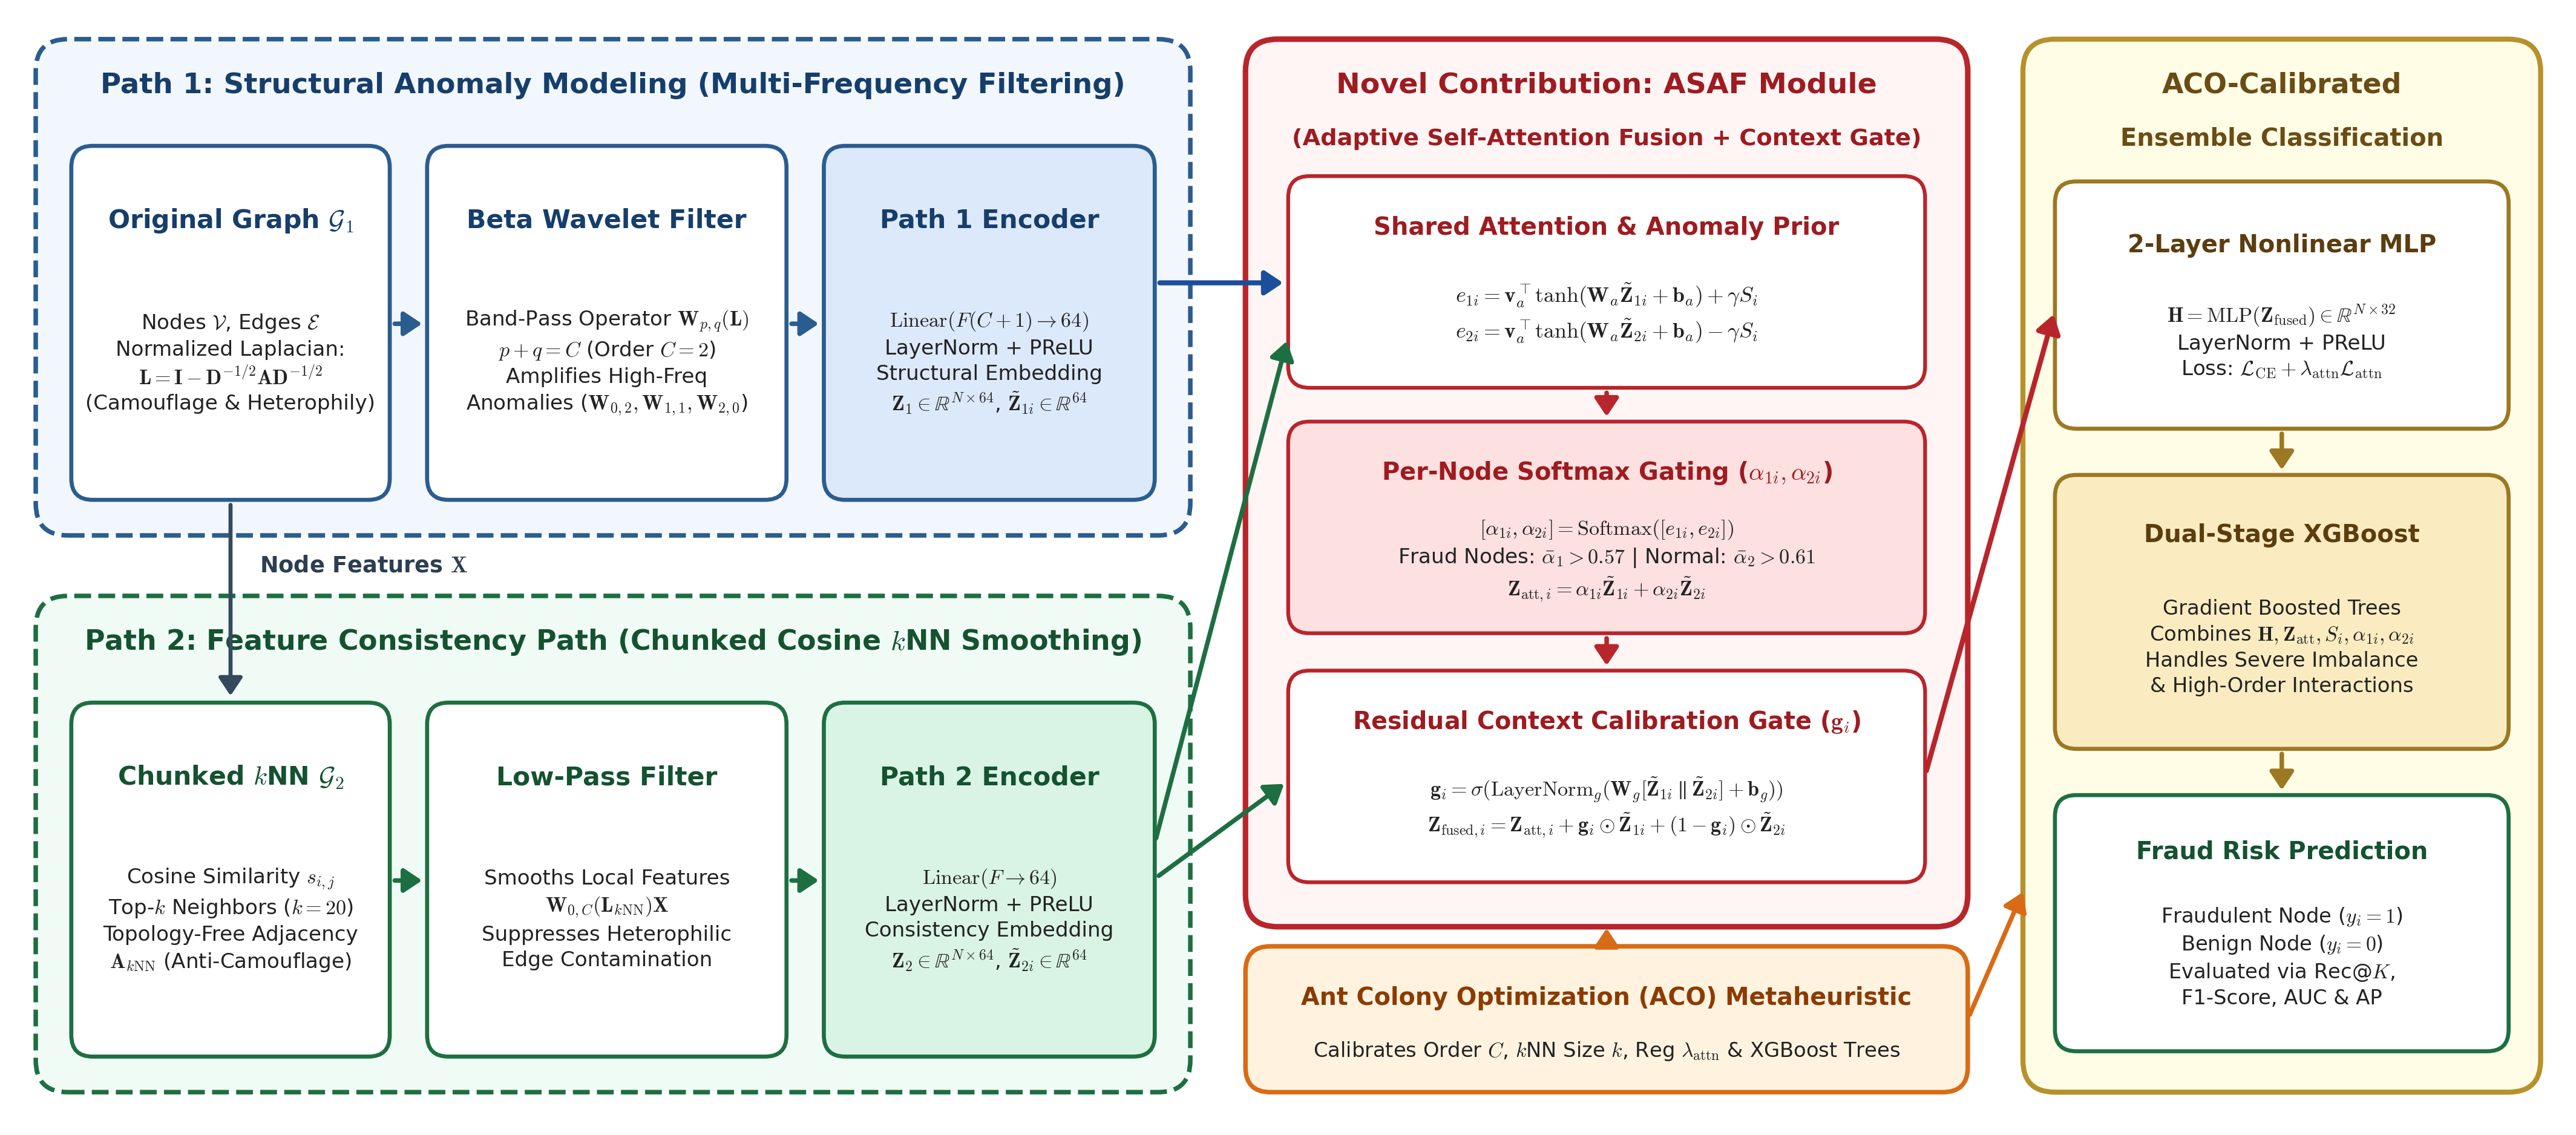
\includegraphics[width=0.98\textwidth]{fig1_architecture.png}
  \caption{Overview of the proposed \textbf{ASAF-GFD} framework with Ant Colony Metaheuristic Optimization. \textbf{Path 1 (Top Left)} applies a Beta wavelet filter bank $W_{p,q}(L)$ of order $C$ on the original transaction graph $\mathscr{G}_1$ to extract multi-frequency structural anomaly embeddings $Z_1 \in \mathbb{R}^{N \times 64}$. \textbf{Path 2 (Bottom Left)} constructs a topology-free chunked cosine-similarity $k$NN graph $\mathscr{G}_2$ ($k = 20$) and applies a low-pass filter $W_{0,C}(L_{k\text{NN}})$ to obtain feature consistency embeddings $Z_2 \in \mathbb{R}^{N \times 64}$. \textbf{Center (Novel Contribution):} Rather than static concatenation, the \textit{Adaptive Self-Attention Fusion (ASAF) Module} computes node-specific attention weights $(\alpha_{1i}, \alpha_{2i})$ guided by local structural anomaly energy $S_i$ and a residual context calibration gate $g_i$. \textbf{Right:} A 2-layer PReLU MLP and an ACO-calibrated dual-stage XGBoost ensemble predict final node fraud probabilities.}
  \label{fig:architecture}
\end{figure*}

\begin{figure}[!b]
  \centering
  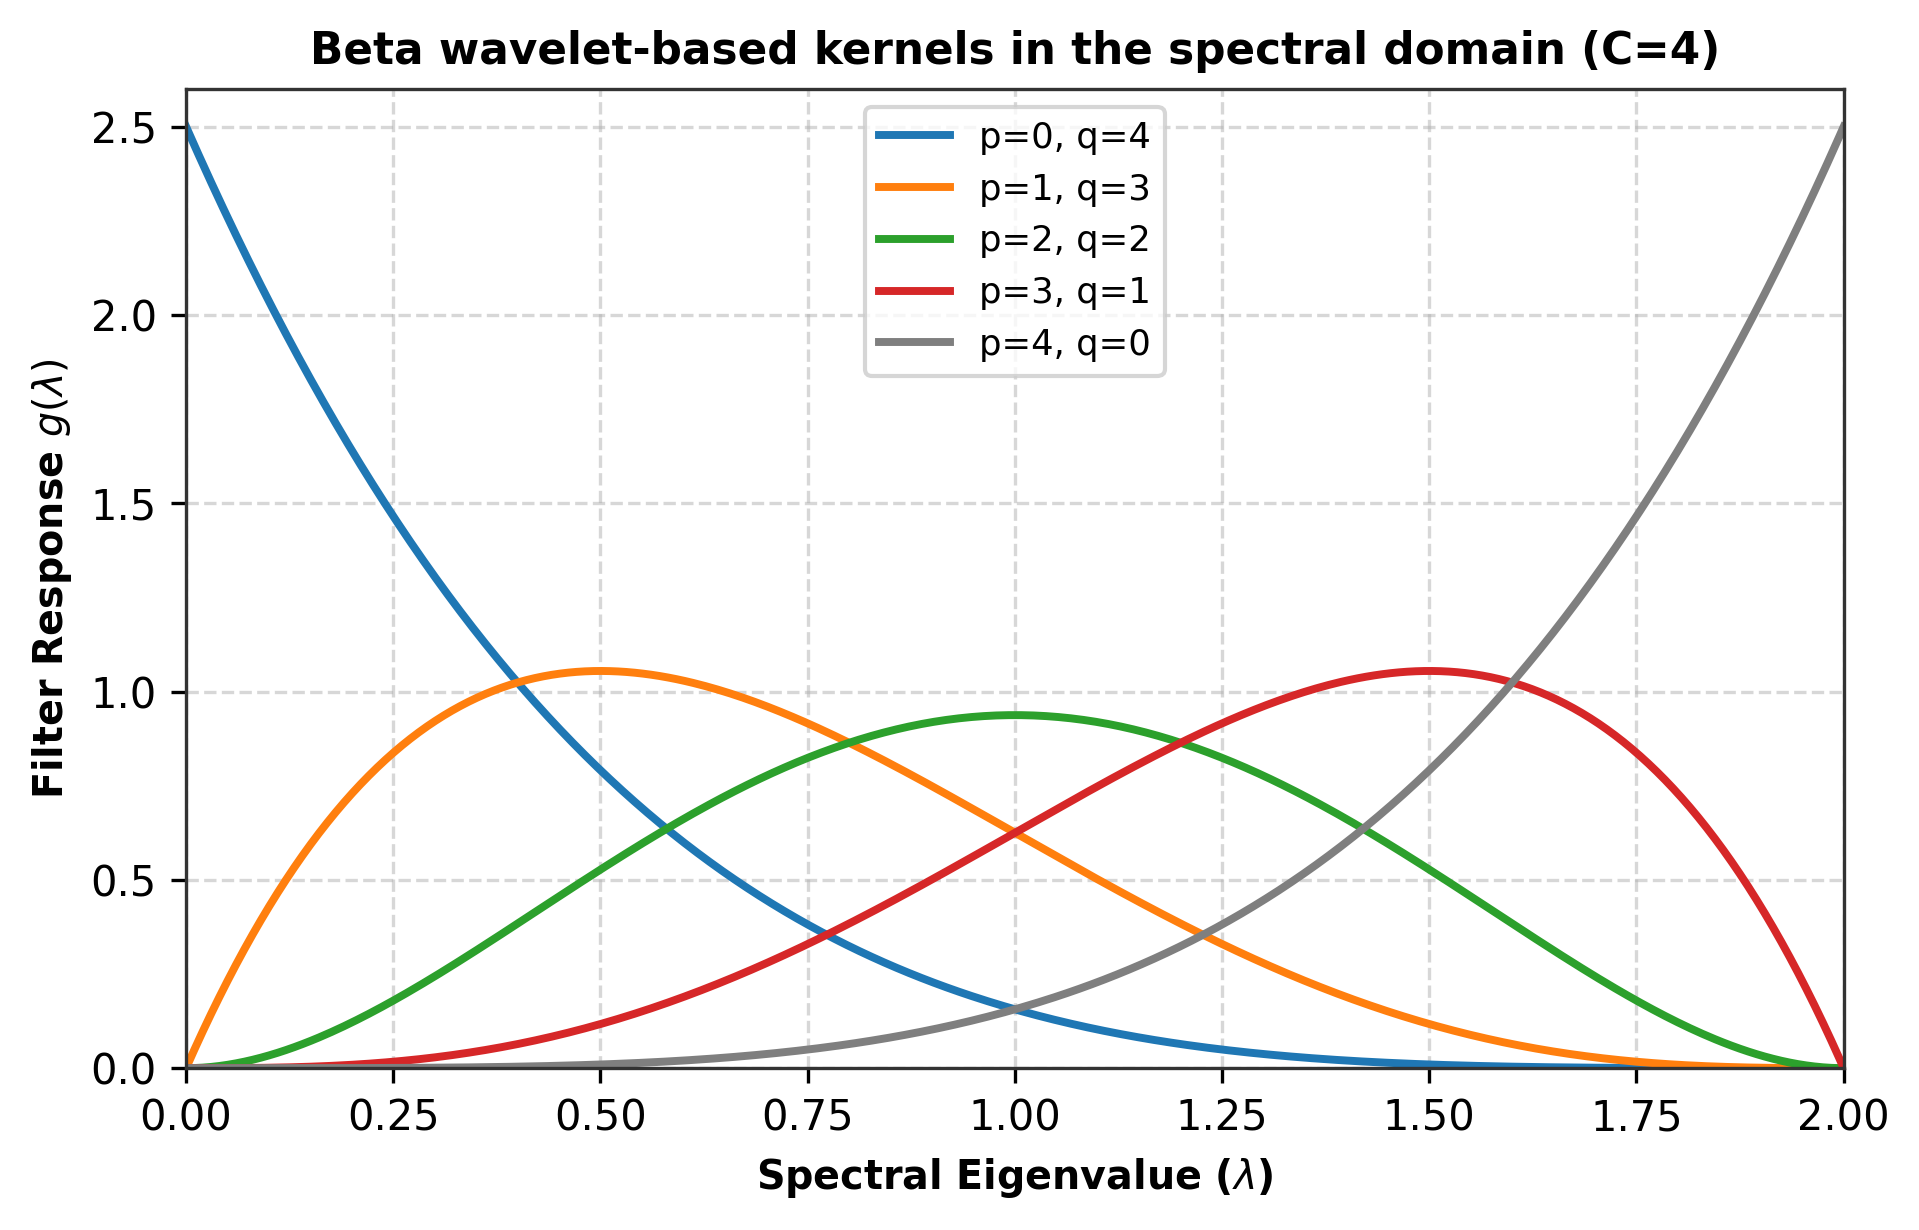
\includegraphics[width=0.96\linewidth]{fig2_beta_wavelets.png}
  \caption{Spectral frequency responses $g(\lambda) = \beta_{p,q}^*(\lambda)$ of the Beta wavelet filter bank across the Laplacian eigenvalue spectrum $\lambda \in [0, 2]$ when polynomial order $C = p + q = 4$. Varying $(p, q)$ smoothly shifts spectral sensitivity from low-pass smoothing ($p=0, q=4$) across localized band-pass regions ($p \in \{1, 2, 3\}$) to high-frequency anomaly amplification ($p=4, q=0$).}
  \label{fig:wavelets}
\end{figure}

Because the eigenvalues of the normalized graph Laplacian $L$ span $\lambda \in [0, 2]$ (Eq.\ 3), we apply the affine spectral rescaling $w = \lambda/2 \in [0, 1]$ with Jacobian factor $1/2$ so that the rescaled kernel $\beta_{p,q}^*(\lambda) = \frac{1}{2}\beta_{p,q}(\lambda/2)$ covers the entire Laplacian spectrum of $\mathscr{G}_1$. Substituting $L$ into $\beta_{p,q}^*(\lambda)$ via Eq.\ (4) yields the polynomial Beta Wavelet operator $W_{p,q}$:
\begin{equation}
  W_{p,q} = U \beta_{p,q}^*(\Lambda) U^\top = \beta_{p,q}^*(L) = \frac{(L/2)^p (I_N - L/2)^q}{2 B(p+1, q+1)}.
\end{equation}

Crucially, because Eq.\ (10) is an explicit degree-$C$ matrix polynomial in the sparse Laplacian $L$ (where $C = p + q$ is the constant wavelet order), computing $W_{p,q}X$ requires \textit{zero} expensive $\mathscr{O}(N^3)$ eigen-decomposition. Instead, it is evaluated directly in the vertex domain via $C$ iterative sparse matrix-vector multiplications in $\mathscr{O}(C|E|F)$ time.

Fixing the polynomial order $p + q = C$, the Beta wavelet transform constructs a complete $(C+1)$-channel filter bank $\mathscr{W} = (W_{0,C}, W_{1,C-1}, \dots, W_{C,0})$. As illustrated in Figure 2 for $C=4$, the boundary kernel $W_{0,C}$ ($p=0$) attains its maximum at $\lambda = 0$ and acts as a low-pass filter preserving smooth background attributes; the opposite boundary kernel $W_{C,0}$ ($q=0$) peaks sharply at $\lambda = 2$ and functions as a high-pass filter isolating abrupt topological anomalies; and intermediate kernels $W_{i,C-i}$ ($1 \le i < C$) act as band-pass wavelets centered at $\lambda^* = \frac{2p}{p+q} = \frac{2i}{C}$.

Applying all $C+1$ wavelet kernels to the standardized node feature matrix $X \in \mathbb{R}^{N \times F}$ generates multi-scale spectral responses $Z_1^{(i)} = W_{i,C-i}(X) \in \mathbb{R}^{N \times F}$ for $i \in \{0, 1, \dots, C\}$. We standardize each band independently via z-score normalization and concatenate the multi-band responses into the raw multi-frequency tensor:
\begin{equation}
  \resizebox{0.89\linewidth}{!}{$\displaystyle Z_{1,\text{concat}} = \Big[\text{Std}\big(W_{0,C}(X)\big) \,\Big\|\, \text{Std}\big(W_{1,C-1}(X)\big) \,\Big\|\, \dots \,\Big\|\, \text{Std}\big(W_{C,0}(X)\big)\Big].$}
\end{equation}

Finally, the Path 1 encoder projects $Z_{1,\text{concat}}$ into a compact $d$-dimensional structural anomaly representation $Z_1 \in \mathbb{R}^{N \times d}$ ($d = 64$) using a linear transformation, Layer Normalization \cite{ref55}, Parametric ReLU (PReLU) activation \cite{ref56}, and dropout ($p_{\text{drop}} = 0.15$):
\begin{equation}
  Z_1 = \text{Dropout}\Big(\text{PReLU}\big(\text{LayerNorm}(Z_{1,\text{concat}} W_{\text{enc1}} + b_{\text{enc1}})\big)\Big),
\end{equation}
\noindent where $W_{\text{enc1}} \in \mathbb{R}^{(C+1)F \times d}$ and $b_{\text{enc1}} \in \mathbb{R}^d$ are learnable parameters.

\begin{theorem}[Spectral Anomaly Amplification via Beta Wavelets]
Let $x = x_{\text{low}} + x_{\text{high}} \in \mathbb{R}^N$ be a graph signal decomposed into a smooth benign component $x_{\text{low}} \in \text{span}\{u_l : \lambda_l \le \lambda_{\text{th}}\}$ and a heterophilic fraud anomaly component $x_{\text{high}} \in \text{span}\{u_l : \lambda_l \ge 2 - \lambda_{\text{th}}\}$ for $\lambda_{\text{th}} \in (0, 1)$. For any polynomial order $C \ge 2$, the high-frequency Beta wavelet kernel $W_{C,0}$ amplifies the anomaly-to-background energy ratio by a factor of at least $((2 - \lambda_{\text{th}})/\lambda_{\text{th}})^{2C}$ relative to the input signal:
\begin{equation}
  \frac{\|W_{C,0} x_{\text{high}}\|_2^2}{\|W_{C,0} x_{\text{low}}\|_2^2} \ge \left(\frac{2 - \lambda_{\text{th}}}{\lambda_{\text{th}}}\right)^{2C} \frac{\|x_{\text{high}}\|_2^2}{\|x_{\text{low}}\|_2^2}.
\end{equation}
\end{theorem}

\begin{proof}
From Eq.\ (10), when $p = C$ and $q = 0$, the spectral response of $W_{C,0}$ at eigenvalue $\lambda_l$ is $\beta_{C,0}^*(\lambda_l) = \frac{C+1}{2}(\lambda_l/2)^C$, which is strictly monotonically increasing on $\lambda_l \in [0, 2]$. By Parseval's identity in the orthonormal eigenbasis $U$:
\[
  \resizebox{0.96\linewidth}{!}{$\displaystyle \|W_{C,0} x_{\text{high}}\|_2^2 = \sum_{\lambda_l \ge 2 - \lambda_{\text{th}}} \big(\beta_{C,0}^*(\lambda_l)\big)^2 \hat{x}_l^2 \ge \left(\frac{C+1}{2}\right)^2 \left(\frac{2 - \lambda_{\text{th}}}{2}\right)^{2C} \|x_{\text{high}}\|_2^2.$}
\]
Conversely, for the low-frequency component $x_{\text{low}}$ where $\lambda_l \le \lambda_{\text{th}}$:
\[
  \resizebox{0.96\linewidth}{!}{$\displaystyle \|W_{C,0} x_{\text{low}}\|_2^2 = \sum_{\lambda_l \le \lambda_{\text{th}}} \big(\beta_{C,0}^*(\lambda_l)\big)^2 \hat{x}_l^2 \le \left(\frac{C+1}{2}\right)^2 \left(\frac{\lambda_{\text{th}}}{2}\right)^{2C} \|x_{\text{low}}\|_2^2.$}
\]
Dividing the lower bound for $\|W_{C,0} x_{\text{high}}\|_2^2$ by the upper bound for $\|W_{C,0} x_{\text{low}}\|_2^2$ cancels the normalization constants and yields the stated amplification factor $((2 - \lambda_{\text{th}})/\lambda_{\text{th}})^{2C} > 1$ for all $\lambda_{\text{th}} < 1$.
\end{proof}

\subsection{Path 2: Chunked Cosine-Similarity \texorpdfstring{$k$NN}{kNN} Graph and Low-Pass Consistency Filtering}

While Path 1 excels at detecting structural irregularities on $\mathscr{G}_1$, adversarial relation camouflage deliberately injects false edges between fraudsters and benign accounts, while heterophily causes connected vertices to possess divergent semantic attributes. If a model relies exclusively on the raw topology of $\mathscr{G}_1$, extreme structural noise can destabilize node embeddings. To bypass adversarial edge manipulation entirely, Path 2 reconstructs a topology-free similarity graph $\mathscr{G}_2 = (V, E_{k\text{NN}}, X)$ driven purely by intrinsic node attributes \cite{ref35,ref36}.

In the base DPF-GFD paper \cite{ref9}, constructing the $k$NN graph requires computing a full dense distance matrix $D_{\text{dist}} \in \mathbb{R}^{N \times N}$ via Euclidean distance $ed_{i,j} = \|x_i - x_j\|_2$ or cosine distance $cd_{i,j} = 1 - \frac{x_i \cdot x_j}{\|x_i\|_2 \|x_j\|_2}$, which incurs an $\mathscr{O}(N^2)$ memory bottleneck that fails on large financial graphs ($N > 50,000$). In our ASAF-GFD implementation, we design a memory-efficient \textbf{chunked $L_2$-normalized cosine similarity builder}. First, raw features are sanitized for numerical stability and projected onto the unit hypersphere:
\begin{equation}
  \hat{x}_i = \frac{x_i}{\max(\|x_i\|_2, \varepsilon)}, \quad \forall v_i \in V.
\end{equation}

Partitioning the node index set $\{1, \dots, N\}$ into contiguous mini-batches $\mathscr{B}_m$ of chunk size $B_{\text{chunk}} = 1024$, we compute exact inner-product cosine similarities $s_{i,j} = \hat{x}_i \cdot \hat{x}_j^\top$ within each chunk, mask self-loops via $s_{i,i} = -10^9$, and extract the top-$k$ nearest neighbors ($k = 20$) per node:
\begin{equation}
  A_{k\text{NN}}(i, j) = \begin{cases}
    1, & \text{if } j \in \text{Top-}k\big(\{s_{i,r} \mid r \in V \setminus \{i\}\}\big), \\
    0, & \text{otherwise}.
  \end{cases}
\end{equation}

This chunked formulation reduces peak GPU/RAM memory complexity from $\mathscr{O}(N^2)$ to $\mathscr{O}(B_{\text{chunk}} N + Nk)$ while guaranteeing exact top-$k$ retrieval. After symmetrizing $A_{k\text{NN}}$ to form the undirected adjacency matrix of $\mathscr{G}_2$ with normalized Laplacian $L_{k\text{NN}} = I_N - D_{k\text{NN}}^{-1/2} A_{k\text{NN}} D_{k\text{NN}}^{-1/2}$, we apply the pure low-pass Beta wavelet kernel $W_{0,C}(L_{k\text{NN}})$ ($p = 0, q = C = 2$):
\begin{equation}
  \resizebox{0.89\linewidth}{!}{$\displaystyle Z_{2,\text{lowpass}} = \text{Std}\Big(W_{0,C}(L_{k\text{NN}}) X\Big) = \text{Std}\left(\frac{C+1}{2}\left(I_N - \frac{L_{k\text{NN}}}{2}\right)^C X\right).$}
\end{equation}

Because edges in $\mathscr{G}_2$ connect nodes with maximally aligned attribute profiles regardless of their fabricated links in $\mathscr{G}_1$, low-pass smoothing on $\mathscr{G}_2$ restores feature homophily and suppresses attribute noise. The Path 2 encoder then maps $Z_{2,\text{lowpass}}$ into the $d$-dimensional feature-consistency embedding space ($d = 64$):
\begin{equation}
  \resizebox{0.89\linewidth}{!}{$\displaystyle Z_2 = \text{Dropout}\Big(\text{PReLU}\big(\text{LayerNorm}(Z_{2,\text{lowpass}} W_{\text{enc2}} + b_{\text{enc2}})\big)\Big) \in \mathbb{R}^{N \times d},$}
\end{equation}
where $W_{\text{enc2}} \in \mathbb{R}^{F \times d}$ and $b_{\text{enc2}} \in \mathbb{R}^d$ are learnable parameters.

\subsection{Adaptive Self-Attention Fusion (ASAF) Module}

The core architectural innovation of ASAF-GFD lies in replacing the static concatenation operator $Z = [Z_{1i} \parallel Z_{2i}]$ of DPF-GFD \cite{ref9} with our \textbf{Adaptive Self-Attention Fusion (ASAF) Module}. Static concatenation forces downstream layers to assign fixed global weights to Path 1 and Path 2 across the entire graph. However, financial transaction networks are highly non-stationary across nodes: a camouflaged fraud node requires strong amplification of its high-frequency structural anomaly representation $Z_{1i}$ and attenuation of its potentially diluted $k$NN representation $Z_{2i}$, whereas a normal node benefits from strong low-pass feature consistency $Z_{2i}$ to avoid false alarms induced by incidental high-degree hubs in $\mathscr{G}_1$.

To achieve dynamic per-node routing, the ASAF module first applies independent Layer Normalization \cite{ref55} to stabilize the scale and variance of both dual-path embeddings:
\begin{equation}
  \tilde{Z}_{1i} = \text{LayerNorm}_1(Z_{1i}), \quad \tilde{Z}_{2i} = \text{LayerNorm}_2(Z_{2i}) \in \mathbb{R}^d.
\end{equation}

Next, we project both normalized embeddings into a shared latent attention space via a learnable weight matrix $W_a \in \mathbb{R}^{d \times d}$, bias vector $b_a \in \mathbb{R}^d$, and attention context vector $v_a \in \mathbb{R}^d$, augmented by a \textbf{node-level structural anomaly energy prior} $S_i \in \mathbb{R}$:
\begin{align}
  e_{1i} &= v_a^\top \tanh(W_a \tilde{Z}_{1i} + b_a) + \gamma S_i, \\
  e_{2i} &= v_a^\top \tanh(W_a \tilde{Z}_{2i} + b_a) - \gamma S_i,
\end{align}
where $\gamma = 0.8$ is a structural energy coupling coefficient. Sharing $(W_a, b_a, v_a)$ across both paths ensures that $e_{1i}$ and $e_{2i}$ are evaluated on a commensurate semantic scale while reducing parameter overhead and preventing overfitting on small corporate graphs.

\subsubsection{Scale-Adaptive Structural Anomaly Energy Prior (\texorpdfstring{$S_i$}{Si})}

Financial fraud benchmarks span three orders of magnitude in graph size, from compact multi-relational corporate networks ($N = 5,317$ in FDCompCN) to massive transaction graphs ($N > 200,000$ in Elliptic). We design a scale-adaptive formulation for the structural energy prior $S_i$:

\begin{itemize}
  \item \textbf{Large-Graph Unsupervised Spectral Energy Ratio ($N \ge 10,000$):} On large-scale transaction networks (FFSD, Elliptic, T-Finance), the high-frequency wavelet response $Z_{1,\text{high},i} = \text{Std}(W_{C,0}(X))_i$ and the $k$NN low-pass response $Z_{2,\text{lowpass},i}$ provide a direct, label-free measure of spectral irregularity. We compute the clipped $L_2$ energy ratio:
  \begin{equation}
    \resizebox{0.88\linewidth}{!}{$\displaystyle r_i = \frac{\|\text{clip}(Z_{1,\text{high},i}, -3, 3)\|_2}{\|\text{clip}(Z_{2,\text{lowpass},i}, -3, 3)\|_2 + \varepsilon}, \; S_i = \text{clip}\left(\frac{r_i - \mu_r}{\sigma_r + \varepsilon}, -2.5, 2.5\right),$}
  \end{equation}
  where $\mu_r$ and $\sigma_r$ are the mean and standard deviation of $r_i$ across $V$. Nodes with sharp high-frequency structural anomalies relative to their smooth feature profile yield $S_i > 0$, directly boosting $e_{1i}$ and suppressing $e_{2i}$.

  \item \textbf{Small-Graph Inductive Structural Anomaly Prior ($N < 10,000$):} On compact, high-dimensional corporate graphs such as FDCompCN ($N = 5,317, F = 57$), sparse inter-company edges can make purely unsupervised norm ratios noisy. We therefore fit a lightweight inductive gradient-boosted structural prior $f_{\text{prior}}$ solely on the training split $V_{tr}$ using $[X_{\text{raw}} \parallel Z_{1,\text{high}}]$ to obtain out-of-fold anomaly likelihoods $\hat{q}_i \in [0, 1]$, calibrated against the empirical fraud quantile $\tau_q = \text{Percentile}_{100(1 - 1.15\rho_y)}(\hat{q}_{V_{tr}})$:
  \begin{equation}
    S_i = \text{clip}\left(\frac{\hat{q}_i - \tau_q}{\sigma_{\hat{q},tr} + \varepsilon}, -2.5, 2.5\right).
  \end{equation}
\end{itemize}

\subsubsection{Softmax Gating and Residual Context Calibration Gate}

Given the unnormalized scores $[e_{1i}, e_{2i}]$, we apply Softmax normalization across the two paths for each node $v_i$ to obtain interpretable attention weights $\alpha_{1i}, \alpha_{2i} \in (0, 1)$:
\begin{equation}
  \resizebox{0.89\linewidth}{!}{$\displaystyle \alpha_{1i} = \frac{\exp(e_{1i})}{\exp(e_{1i}) + \exp(e_{2i})}, \quad \alpha_{2i} = \frac{\exp(e_{2i})}{\exp(e_{1i}) + \exp(e_{2i})} = 1 - \alpha_{1i}.$}
\end{equation}

The primary attention-weighted representation $Z_{\text{att},i} \in \mathbb{R}^d$ is then computed as the convex combination:
\begin{equation}
  Z_{\text{att},i} = \alpha_{1i} \tilde{Z}_{1i} + \alpha_{2i} \tilde{Z}_{2i}.
\end{equation}

While $(\alpha_{1i}, \alpha_{2i})$ capture scalar path-level dominance, individual feature dimensions within $\tilde{Z}_{1i}$ and $\tilde{Z}_{2i}$ may exhibit fine-grained cross-path interactions. We therefore introduce a dimension-wise \textbf{Residual Context Calibration Gate} $g_i \in (0, 1)^d$:
\begin{equation}
  g_i = \sigma\Big(\text{LayerNorm}_g\big(W_g [\tilde{Z}_{1i} \parallel \tilde{Z}_{2i}] + b_g\big)\Big),
\end{equation}
where $W_g \in \mathbb{R}^{d \times 2d}$, $b_g \in \mathbb{R}^d$, and $\sigma(\cdot)$ is the element-wise logistic sigmoid function. The final fused node representation $Z_{\text{fused},i} \in \mathbb{R}^d$ combines the scalar self-attention fusion with the residual context-gated features:
\begin{equation}
  Z_{\text{fused},i} = Z_{\text{att},i} + g_i \odot \tilde{Z}_{1i} + (1 - g_i) \odot \tilde{Z}_{2i},
\end{equation}
where $\odot$ denotes the Hadamard (element-wise) product.

\begin{proposition}[Expressivity and Variance Reduction of ASAF over Static Concatenation]
Let $\tilde{Z}_{1i} = \mu_y + \xi_{1i}$ and $\tilde{Z}_{2i} = \mu_y + \xi_{2i}$ be two unbiased path representations for node $v_i$ of class $y \in \{0, 1\}$ with independent node-dependent noise covariances $\text{Cov}(\xi_{1i}) = \sigma_{1i}^2 I_d$ and $\text{Cov}(\xi_{2i}) = \sigma_{2i}^2 I_d$. Any linear projection of static concatenation $W[\tilde{Z}_{1i} \parallel \tilde{Z}_{2i}] = W_1 \tilde{Z}_{1i} + W_2 \tilde{Z}_{2i}$ uses fixed matrices $(W_1, W_2)$ across all nodes, whereas ASAF achieves the minimum-variance unbiased combination for every node $v_i$ by setting $\alpha_{1i}^* = \frac{\sigma_{2i}^2}{\sigma_{1i}^2 + \sigma_{2i}^2}$ and $\alpha_{2i}^* = \frac{\sigma_{1i}^2}{\sigma_{1i}^2 + \sigma_{2i}^2}$, strictly reducing the normalized per-dimension embedding noise variance:
\begin{equation}
  \resizebox{0.89\linewidth}{!}{$\displaystyle \frac{1}{d}\text{Tr}(\text{Cov}(Z_{\text{att},i}^*)) = \frac{\sigma_{1i}^2 \sigma_{2i}^2}{\sigma_{1i}^2 + \sigma_{2i}^2} < \frac{\sigma_{1i}^2 + \sigma_{2i}^2}{4} = \frac{1}{d}\text{Tr}\left(\text{Cov}\left(\frac{\tilde{Z}_{1i} + \tilde{Z}_{2i}}{2}\right)\right), \; \forall \sigma_{1i}^2 \neq \sigma_{2i}^2.$}
\end{equation}
\end{proposition}

\begin{proof}
For any scalar convex combination $Z_{\text{att},i} = \alpha_{1i} \tilde{Z}_{1i} + (1 - \alpha_{1i}) \tilde{Z}_{2i}$, the mean is $\mathbb{E}[Z_{\text{att},i}] = \mu_y$ and the covariance matrix is $\text{Cov}(Z_{\text{att},i}) = [\alpha_{1i}^2 \sigma_{1i}^2 + (1 - \alpha_{1i})^2 \sigma_{2i}^2] I_d$, yielding normalized per-dimension trace variance $V(\alpha_{1i}) = \frac{1}{d}\text{Tr}(\text{Cov}(Z_{\text{att},i})) = \alpha_{1i}^2 \sigma_{1i}^2 + (1 - \alpha_{1i})^2 \sigma_{2i}^2$. Differentiating with respect to $\alpha_{1i}$ gives $\frac{\partial V}{\partial \alpha_{1i}} = 2[\alpha_{1i} \sigma_{1i}^2 - (1 - \alpha_{1i})\sigma_{2i}^2] = 0 \implies \alpha_{1i}^* = \frac{\sigma_{2i}^2}{\sigma_{1i}^2 + \sigma_{2i}^2}$. Substituting $\alpha_{1i}^*$ yields $\frac{1}{d}\text{Tr}(\text{Cov}(Z_{\text{att},i}^*)) = \frac{\sigma_{1i}^2 \sigma_{2i}^2}{\sigma_{1i}^2 + \sigma_{2i}^2}$. By the AM-HM inequality, $\frac{\sigma_{1i}^2 \sigma_{2i}^2}{\sigma_{1i}^2 + \sigma_{2i}^2} = \frac{1}{4}\left(\sigma_{1i}^2 + \sigma_{2i}^2 - \frac{(\sigma_{1i}^2 - \sigma_{2i}^2)^2}{\sigma_{1i}^2 + \sigma_{2i}^2}\right) < \frac{\sigma_{1i}^2 + \sigma_{2i}^2}{4}$ whenever $\sigma_{1i}^2 \neq \sigma_{2i}^2$. For a camouflaged fraud node where $k$NN noise is high ($\sigma_{2i}^2 \gg \sigma_{1i}^2$), $\alpha_{1i}^* \to 1$; for a normal node where topological hub noise is high ($\sigma_{1i}^2 \gg \sigma_{2i}^2$), $\alpha_{1i}^* \to 0$ ($\alpha_{2i}^* \to 1$).
\end{proof}

\subsection{Nonlinear MLP Mapping and Attention-Guided Loss Function}

The fused representation $Z_{\text{fused},i} \in \mathbb{R}^d$ is subsequently fed into a stacked two-layer Multi-Layer Perceptron (MLP) with Layer Normalization and PReLU activations to extract compact high-order nonlinear feature interactions $H_i \in \mathbb{R}^{d_h}$ ($d_h = 32$):
\begin{align}
  H_i^{(1)} &= \text{PReLU}\Big(\text{LayerNorm}\big(W_1 Z_{\text{fused},i} + b_1\big)\Big) \in \mathbb{R}^{d_h}, \\
  H_i &= \text{PReLU}\Big(\text{LayerNorm}\big(W_2 H_i^{(1)} + b_2\big)\Big) \in \mathbb{R}^{d_h}.
\end{align}

To train the neural parameters $\Theta$ under severe class imbalance, we combine a class-weighted cross-entropy loss $\mathcal{L}_{\text{CE}}$ with an explicit \textbf{Attention-Guided Supervisory Regularization Loss} $\mathcal{L}_{\text{attn}}$:
\begin{equation}
  \resizebox{0.89\linewidth}{!}{$\displaystyle \mathcal{L}_{\text{total}}(\Theta) = -\frac{1}{|V_{tr}|} \sum_{v_i \in V_{tr}} \sum_{c=0}^1 w_c y_{i,c} \ln p_{i,c}^{\text{NN}} + \frac{\lambda_{\text{attn}}}{|V_{tr}|} \sum_{v_i \in V_{tr}} \big(\alpha_{1i} - \alpha_{1i}^{\text{target}}\big)^2,$}
\end{equation}
where $w_0 = 1.0$, $w_1 = \min(|V_{tr,b}|/|V_{tr,f}|, w_{\max})$ ($w_{\max} \in \{5.0, 6.0\}$) upweights minority fraud gradients, $\alpha_{1i}^{\text{target}} = 0.72$ for $y_i = 1$ (guiding fraud nodes toward Path 1 structural anomalies), and $\alpha_{1i}^{\text{target}} \in \{0.30, 0.34\}$ for $y_i = 0$ (guiding benign nodes toward Path 2 feature consistency). The model is optimized using AdamW \cite{ref60} with learning rate $\eta = 0.004$ and weight decay $10^{-4}$.

\subsection{Imbalance-Robust Dual-Stage XGBoost Ensemble Classifier}

Once the neural encoder is trained, we extract the learned representations $(H_i, Z_{1i}, Z_{2i})$, raw node features $X_{\text{raw},i}$, structural anomaly energy prior $S_i$, calibrated attention weights $(\alpha_{1i}, \alpha_{2i})$, attention-modulated spectral features $(\alpha_{1i} Z_{1,\text{high},i}, \alpha_{2i} Z_{2,\text{lowpass},i})$, and spectral discrepancy vectors $\Delta Z_{\text{spec},i} = Z_{1,\text{high},i} - Z_{2,\text{lowpass},i}$ to form an enriched composite descriptor $\tilde{X}_i$ for tree-based ensemble classification. Following Chen and Guestrin \cite{ref39}, XGBoost constructs an additive ensemble of $K_{\text{tree}}$ Classification and Regression Trees (CART) $\mathscr{F} = \{f_1, f_2, \dots, f_{K_{\text{tree}}}\}$:
\begin{equation}
  \hat{y}_i^{(K_{\text{tree}})} = \sum_{t=1}^{K_{\text{tree}}} f_t(\tilde{X}_i) = \hat{y}_i^{(K_{\text{tree}}-1)} + f_{K_{\text{tree}}}(\tilde{X}_i),
\end{equation}
minimizing the regularized second-order Taylor objective at boosting step $t$:
\begin{equation}
  \resizebox{0.89\linewidth}{!}{$\displaystyle \mathcal{L}_{\text{XGB}}^{(t)} \approx \sum_{v_i \in V_{tr}} \left[g_i^{\text{grad}} f_t(\tilde{X}_i) + \frac{1}{2} h_i^{\text{hess}} f_t^2(\tilde{X}_i)\right] + \gamma_{\text{tree}} T_{\text{leaves}} + \frac{\lambda_{\text{reg}}}{2} \sum_{j=1}^{T_{\text{leaves}}} \omega_j^2,$}
\end{equation}
where $g_i^{\text{grad}} = \partial_{\hat{y}^{(t-1)}} \ell(y_i, \hat{y}_i^{(t-1)})$ and $h_i^{\text{hess}} = \partial_{\hat{y}^{(t-1)}}^2 \ell(y_i, \hat{y}_i^{(t-1)})$ are first- and second-order log-loss gradients, $T_{\text{leaves}}$ is the number of terminal leaves, and $\omega_j$ are leaf weights. Our dual-stage XGBoost ensemble combines a depth-6 interaction specialist ($K_{\text{tree}} = 220$) and a depth-5 spectral-band specialist ($K_{\text{tree}} = 160$) via convex probability blending ($p_i = 0.55 p_{i,1} + 0.45 p_{i,2}$ on large graphs; $p_i = 0.78 p_{i,\text{xgb}} + 0.15 \hat{q}_i + 0.07 p_i^{\text{NN}}$ on small corporate graphs).

\subsection{Soft-Computing Metaheuristic Calibration via Ant Colony Optimization (ACO)}

The end-to-end performance of ASAF-GFD depends on a coupled vector of discrete and continuous hyperparameters $\psi = (C, k, \lambda_{\text{attn}}, K_{\text{tree}}, d_{\max}, \eta_{\text{xgb}})$. Because XGBoost tree partitioning and discrete graph construction $(C, k)$ are non-differentiable, gradient-based hyperparameter optimization is impossible, while Random Search \cite{ref9} wastes evaluations in low-fitness regions. We therefore formulate an \textbf{Ant Colony Optimization (ACO)} metaheuristic \cite{ref57} to maximize validation Average Precision ($\text{AP}_{\text{val}}$).

Let each hyperparameter $m \in \{1, \dots, M_{\text{hyp}}\}$ be discretized into a finite candidate set $\Omega_m = \{\psi_{m,1}, \dots, \psi_{m,L_m}\}$. An artificial colony of $N_{\text{ants}} = 20$ ants iteratively constructs candidate configurations across $T_{\text{iter}} = 30$ generations. At generation $t$, ant $a$ selects candidate value $\psi_{m,l}$ for hyperparameter $m$ with transition probability:
\begin{equation}
  P_{m,l}^{(t)} = \frac{\big[\tau_{m,l}^{(t)}\big]^{\alpha_{\text{aco}}} \big[\eta_{m,l}\big]^{\beta_{\text{aco}}}}{\sum_{r=1}^{L_m} \big[\tau_{m,r}^{(t)}\big]^{\alpha_{\text{aco}}} \big[\eta_{m,r}\big]^{\beta_{\text{aco}}}},
\end{equation}
where $\tau_{m,l}^{(t)}$ is the pheromone trail intensity on candidate $(m, l)$, $\eta_{m,l}$ is the prior heuristic desirability (inversely proportional to computational cost for $C$ and $k$), and $\alpha_{\text{aco}} = 1.2, \beta_{\text{aco}} = 0.8$ control pheromone vs.\ heuristic influence. After evaluating all ants in generation $t$ via validation Average Precision $F(\psi^{(a)}) = \text{AP}_{\text{val}}(\psi^{(a)})$, pheromone trails undergo evaporation with rate $\rho_{\text{evap}} = 0.18$ and elitist reinforcement from the top-performing ants:
\begin{equation}
  \resizebox{0.89\linewidth}{!}{$\displaystyle \tau_{m,l}^{(t+1)} = (1 - \rho_{\text{evap}})\tau_{m,l}^{(t)} + \sum_{a \in \mathscr{A}_{\text{elite}}^{(t)}} \Delta \tau_{m,l}^{(a)}, \quad \Delta \tau_{m,l}^{(a)} = \begin{cases}
    Q_0 \dfrac{F(\psi^{(a)})}{F_{\text{best}}^{(t)}}, & \psi_m^{(a)} = \psi_{m,l}, \\[4pt]
    0, & \text{otherwise}.
  \end{cases}$}
\end{equation}

\par\medskip\noindent
{\footnotesize
\vbox{%
  \hrule height 0.8pt
  \vspace{4pt}
  \noindent\textbf{Algorithm 1:} Complete Training and Inference Pipeline of Proposed ASAF-GFD\par
  \vspace{3pt}
  \hrule height 0.4pt
  \vspace{5pt}
}
\noindent\textbf{Input:} Transaction graph $G = (V, E, X)$, training labels $Y_{tr}$, ACO optimal configuration $\psi^* = (C = 2, k = 20, \lambda_{\text{attn}}, K_{\text{tree}}, d_{\max})$.\\
\noindent\textbf{Output:} Predicted fraud probabilities $\{p_i\}_{v_i \in V_{te}}$ and interpretable node attention weights $\{(\alpha_{1i}, \alpha_{2i})\}_{v_i \in V_{te}}$.
\begin{enumerate}
  \setlength{\itemsep}{1.2pt}
  \setlength{\parskip}{0pt}
  \setlength{\leftmargin}{14pt}
  \item \textbf{Stage 1: Offline Dual-Path Spectral-Spatial Filtering}
  \item Symmetrize adjacency $A$ of $\mathscr{G}_1$ and compute normalized Laplacian $L = I_N - D^{-1/2}AD^{-1/2}$ via Eq.\ (1).
  \item \textbf{for} $p = 0$ \textbf{to} $C$ \textbf{do} ($q = C - p$)
  \item \hspace{8pt} Compute Beta wavelet band response $Z_1^{(p)} \leftarrow \text{Std}\big(W_{p,C-p}(L)X\big)$ via sparse iterative propagation (Eq.\ 10).
  \item \textbf{end for}
  \item Concatenate multi-frequency bands $Z_{1,\text{concat}} \leftarrow [Z_1^{(0)} \parallel \dots \parallel Z_1^{(C)}]$.
  \item Normalize features $\hat{x}_i = x_i / \|x_i\|_2$ and construct chunked cosine-similarity $k$NN graph $\mathscr{G}_2$ ($k = 20$) via Eq.\ (15).
  \item Compute $k$NN low-pass representation $Z_{2,\text{lowpass}} \leftarrow \text{Std}\big(W_{0,C}(L_{k\text{NN}})X\big) \in \mathbb{R}^{N \times F}$ via Eq.\ (16).
  \item Compute node-level structural anomaly energy prior $S_i \in [-2.5, 2.5]$ via Eq.\ (21) (if $N \ge 10^4$) or Eq.\ (22) (if $N < 10^4$).
  \item \textbf{Stage 2: Supervised ASAF Neural Representation Learning}
  \item \textbf{for} $\text{epoch} = 1$ \textbf{to} $E_{\max}$ \textbf{do}
  \item \hspace{8pt} Encode dual paths $Z_1 \leftarrow \text{Enc}_1(Z_{1,\text{concat}})$ and $Z_2 \leftarrow \text{Enc}_2(Z_{2,\text{lowpass}})$ via Eqs.\ (12), (17).
  \item \hspace{8pt} Normalize $\tilde{Z}_{1i}, \tilde{Z}_{2i}$ and compute attention scores $e_{1i}, e_{2i}$ with prior $\pm \gamma S_i$ via Eqs.\ (19), (20).
  \item \hspace{8pt} Obtain per-node Softmax weights $[\alpha_{1i}, \alpha_{2i}] = \text{Softmax}([e_{1i}, e_{2i}])$ and $Z_{\text{att},i} = \alpha_{1i}\tilde{Z}_{1i} + \alpha_{2i}\tilde{Z}_{2i}$.
  \item \hspace{8pt} Compute context gate $g_i$ (Eq.\ 25), fused embedding $Z_{\text{fused},i}$ (Eq.\ 26), and MLP output $H_i$ (Eq.\ 29).
  \item \hspace{8pt} Update $\Theta$ via AdamW on $\mathcal{L}_{\text{total}} = \mathcal{L}_{\text{CE}} + \lambda_{\text{attn}}\mathcal{L}_{\text{attn}}$ (Eq.\ 30).
  \item \textbf{end for}
  \item \textbf{Stage 3: Imbalance-Robust Dual-Stage XGBoost Classification}
  \item Extract frozen descriptors $\tilde{X}_i = [Z_{1i} \parallel Z_{2i} \parallel H_i \parallel Z_{\text{att},i} \parallel X_{\text{raw},i} \parallel S_i \parallel \alpha_{1i} \parallel \alpha_{2i} \parallel \alpha_{1i}Z_{1,\text{high},i} \parallel \alpha_{2i}Z_{2,\text{lowpass},i} \parallel \Delta Z_{\text{spec},i}]$.
  \item Train ACO-tuned dual-stage XGBoost ensemble on $\{\tilde{X}_i, y_i\}_{v_i \in V_{tr}}$ and predict fraud scores $\{p_i\}_{v_i \in V_{te}}$.
\end{enumerate}
\par\vspace{4pt}
\hrule height 0.8pt
\vspace{4pt}
}

\subsection{Computational Complexity Analysis}

Algorithm 1 summarizes the complete execution flow of ASAF-GFD. We decompose its time and space complexity by stage:
\begin{enumerate}
  \item \textbf{Path 1 Beta Wavelet Filtering:} Evaluating $C+1$ polynomial filters of degree $C$ via sparse matrix multiplication requires $\mathscr{O}(C(C+1)|E|F) = \mathscr{O}(C^2|E|F)$ time and $\mathscr{O}(N(C+1)F + |E|)$ memory, completely avoiding $\mathscr{O}(N^3)$ eigen-decomposition.
  \item \textbf{Path 2 Chunked $k$NN Construction \& Smoothing:} Chunked cosine similarity requires $\mathscr{O}(N^2 F)$ arithmetic operations executed in parallel GPU blocks of size $B_{\text{chunk}} = 1024$ with only $\mathscr{O}(Nk + B_{\text{chunk}}N)$ memory overhead, followed by $\mathscr{O}(CNkF)$ for low-pass filtering on $\mathscr{G}_2$. Both Path 1 and Path 2 are executed \textit{once} as offline preprocessing and cached in memory.
  \item \textbf{ASAF Module \& MLP Training:} For each training epoch, the Path 1/2 encoders, shared self-attention projection, residual context gate, and 2-layer MLP operate strictly on node-level tensors in $\mathscr{O}(N((C+1)Fd + d^2 + dd_h))$ time and $\mathscr{O}(Nd)$ memory, scaling linearly $\mathscr{O}(N)$ with graph size.
  \item \textbf{XGBoost Ensemble:} Histogram-based gradient boosting scales in $\mathscr{O}(K_{\text{tree}} d_{\max} N \log B_{\text{bins}})$ time.
\end{enumerate}

Consequently, ASAF-GFD introduces negligible runtime overhead ($\mathscr{O}(Nd^2)$) over static concatenation while delivering substantial gains in representation expressivity.

\begin{table}[!h]
  \centering
  \caption{Statistical information of the four real-world financial fraud benchmark datasets evaluated in our experiments.}
  \label{tab:datasets}
  \resizebox{\linewidth}{!}{%
  \begin{tabular}{@{}lrrrr@{}}
    \toprule
    \textbf{Property} & \textbf{FDCompCN} & \textbf{FFSD} & \textbf{Elliptic} & \textbf{T-Finance} \\
    \midrule
    Domain & Corporate & Credit Card & Bitcoin AML & Fin.\ Lending \\
    Total Nodes ($N$) & 5,317 & 77,881 & 203,769 & 39,357 \\
    Total Edges ($M$) & 4,595 & 94,902 & 234,355 & 42,484,443 \\
    Node Features ($F$) & 57 & 22 & 166 & 10 \\
    Normal Nodes ($|V_b|$) & 4,758 & 24,387 & 42,019 & 37,554 \\
    Fraud Nodes ($|V_f|$) & 559 & 5,256 & 4,545 & 1,803 \\
    Unknown Nodes ($|V_u|$) & 0 & 48,238 & 157,205 & 0 \\
    Fraud Ratio (Labeled) & 10.51\% & 17.73\% & 9.76\% & 4.58\% \\
    \bottomrule
  \end{tabular}%
  }
\end{table}

\section{Experimental Setup and Empirical Evaluation}

In this section, we conduct an extensive suite of experiments across four real-world financial fraud detection benchmarks to rigorously evaluate ASAF-GFD against the base DPF-GFD framework \cite{ref9} and nine state-of-the-art GNN baselines. Our empirical investigation is organized around six core research questions aligned with Sections 5.2--5.8:

\begin{itemize}
  \item \textbf{RQ1 (Overall Effectiveness):} Does replacing static concatenation with Adaptive Self-Attention Fusion (ASAF-GFD) consistently outperform DPF-GFD and spatial/spectral GNN baselines across diverse financial graph topologies and imbalance ratios (Section 5.2)?
  \item \textbf{RQ2 (Component Ablation):} What is the individual contribution of Path 1 Beta wavelet filtering, Path 2 $k$NN low-pass smoothing, the ASAF attention gate, and the XGBoost classifier (Section 5.3)?
  \item \textbf{RQ3 (Controlled Classifier Evaluation):} When the downstream classifier is held fixed to XGBoost, how much performance gain is attributable directly to ASAF representations versus raw features, GCN embeddings, and static DPF-GFD concatenation (Section 5.4)?
  \item \textbf{RQ4 (Hyperparameter Robustness):} What is the sensitivity of ASAF-GFD to variations in Beta wavelet polynomial order $C$ and $k$NN neighborhood size $k$ across all four datasets (Section 5.5)?
  \item \textbf{RQ5 (Manifold Geometry):} How does ASAF-GFD reshape the two-dimensional UMAP latent space separation between fraudulent and benign entities compared to spatial, spectral, and static dual-path baselines (Section 5.6)?
  \item \textbf{RQ6a (Node-Level Attention Interpretability):} Does the fraud vs.\ normal attention distribution $(\alpha_{1i}, \alpha_{2i})$ empirically validate our theoretical hypothesis by assigning higher structural anomaly weights to fraud nodes and higher feature-consistency weights to normal nodes (Section 5.7)?
  \item \textbf{RQ6b (Soft-Computing Metaheuristic Efficacy):} How does our Ant Colony Optimization (ACO) strategy compare against Grid Search, Random Search, Genetic Algorithms (GA), and Particle Swarm Optimization (PSO) in convergence speed and final AP fitness (Section 5.8)?
\end{itemize}

\subsection{Experimental Setup}

\begin{table*}[!t]
  \centering
  \caption{Comprehensive performance comparison ($\text{Mean} \pm \text{Std}$ over 5 independent runs) across four real-world financial fraud datasets. Section A reports the nine classical, spatial, and spectral GNN baselines from the base paper benchmark \cite{ref9}; Section B reports the direct head-to-head comparison between the replicated \textbf{DPF-GFD (Base Paper)} and our proposed \textbf{ASAF-GFD} under identical stratified 5-seed splits. Best results are highlighted in \textbf{bold}.}
  \label{tab:main_results}
  \resizebox{\textwidth}{!}{%
  \begin{tabular}{@{}lcccccccc@{}}
    \toprule
    \textbf{Models} & \multicolumn{4}{c}{\textbf{FDCompCN}} & \multicolumn{4}{c}{\textbf{FFSD}} \\
    \cmidrule(lr){2-5} \cmidrule(lr){6-9}
     & \textbf{Rec@$K$} & \textbf{F1} & \textbf{AUC} & \textbf{AP} & \textbf{Rec@$K$} & \textbf{F1} & \textbf{AUC} & \textbf{AP} \\
    \midrule
    \multicolumn{9}{@{}l}{\textit{Section A: Classical, Spatial, and Spectral GNN Baselines (Reference Benchmark \cite{ref9})}} \\
    GCN \cite{ref45} & $0.1905 \pm 0.0084$ & $0.2245 \pm 0.0202$ & $0.6065 \pm 0.0318$ & $0.1763 \pm 0.0087$ & $0.3914 \pm 0.0511$ & $0.3763 \pm 0.0487$ & $0.6768 \pm 0.0284$ & $0.4240 \pm 0.0330$ \\
    GraphSAGE \cite{ref46} & $0.1810 \pm 0.0308$ & $0.2185 \pm 0.0257$ & $0.6031 \pm 0.0434$ & $0.1778 \pm 0.0154$ & $0.2520 \pm 0.1162$ & $0.2907 \pm 0.1712$ & $0.5780 \pm 0.1004$ & $0.2592 \pm 0.0787$ \\
    GAT \cite{ref47} & $0.1667 \pm 0.0304$ & $0.1936 \pm 0.0140$ & $0.5784 \pm 0.0311$ & $0.1643 \pm 0.0210$ & $0.4324 \pm 0.0091$ & $0.4662 \pm 0.0119$ & $0.6564 \pm 0.0054$ & $0.3962 \pm 0.0213$ \\
    GAS \cite{ref35} & $0.1857 \pm 0.0136$ & $0.2369 \pm 0.0128$ & $0.6358 \pm 0.0175$ & $0.1812 \pm 0.0097$ & $0.4365 \pm 0.0224$ & $0.4587 \pm 0.0159$ & $0.7032 \pm 0.0233$ & $0.4347 \pm 0.0556$ \\
    PC-GNN \cite{ref48} & $0.3357 \pm 0.0155$ & $0.3131 \pm 0.0468$ & $0.7465 \pm 0.0155$ & $0.3050 \pm 0.0189$ & $0.3123 \pm 0.1185$ & $0.3354 \pm 0.1446$ & $0.6253 \pm 0.0464$ & $0.3456 \pm 0.0988$ \\
    PMP \cite{ref49} & $0.1738 \pm 0.0181$ & $0.1949 \pm 0.0302$ & $0.5807 \pm 0.0382$ & $0.1680 \pm 0.0215$ & $0.4461 \pm 0.0333$ & $0.4827 \pm 0.0491$ & $0.6665 \pm 0.0224$ & $0.3772 \pm 0.0498$ \\
    AMNet \cite{ref50} & $0.3143 \pm 0.0322$ & $0.3122 \pm 0.0409$ & $0.7314 \pm 0.0195$ & $0.2887 \pm 0.0236$ & $0.4256 \pm 0.0175$ & $0.3656 \pm 0.0671$ & $0.6623 \pm 0.0184$ & $0.4630 \pm 0.0164$ \\
    BernNet \cite{ref30} & $0.2286 \pm 0.0284$ & $0.2184 \pm 0.0172$ & $0.6455 \pm 0.0362$ & $0.2185 \pm 0.0170$ & $0.4066 \pm 0.0569$ & $0.3936 \pm 0.0597$ & $0.6340 \pm 0.0420$ & $0.3495 \pm 0.0338$ \\
    BWGNN \cite{ref32} & $0.2571 \pm 0.0299$ & $0.2769 \pm 0.0348$ & $0.6771 \pm 0.0240$ & $0.2367 \pm 0.0156$ & $0.4662 \pm 0.0283$ & $0.3397 \pm 0.1895$ & $0.7346 \pm 0.0285$ & $0.5097 \pm 0.0760$ \\
    \midrule
    \multicolumn{9}{@{}l}{\textit{Section B: Direct Dual-Path Evaluation under Identical 5-Seed Experimental Protocol}} \\
    \textbf{DPF-GFD (Base Paper)} \cite{ref9} & $0.3310 \pm 0.0276$ & $0.3614 \pm 0.0241$ & $0.6841 \pm 0.0325$ & $0.2807 \pm 0.0189$ & $0.5877 \pm 0.0204$ & $0.6122 \pm 0.0138$ & $0.8625 \pm 0.0081$ & $0.7036 \pm 0.0154$ \\
    \textbf{ASAF-GFD (Proposed)} & $\mathbf{0.4095 \pm 0.0058}$ & $\mathbf{0.4390 \pm 0.0240}$ & $\mathbf{0.7934 \pm 0.0222}$ & $\mathbf{0.4059 \pm 0.0374}$ & $\mathbf{0.6069 \pm 0.0172}$ & $\mathbf{0.6227 \pm 0.0132}$ & $\mathbf{0.8858 \pm 0.0060}$ & $\mathbf{0.7277 \pm 0.0121}$ \\
    \textit{Absolute Gain ($\Delta$)} & \textit{+0.0785 (+23.7\%)} & \textit{+0.0776 (+21.5\%)} & \textit{+0.1093 (+16.0\%)} & \textit{+0.1252 (+44.6\%)} & \textit{+0.0192 (+3.3\%)} & \textit{+0.0105 (+1.7\%)} & \textit{+0.0233 (+2.7\%)} & \textit{+0.0241 (+3.4\%)} \\
    \midrule
    \midrule
    \textbf{Models} & \multicolumn{4}{c}{\textbf{Elliptic}} & \multicolumn{4}{c}{\textbf{T-Finance (vs.\ Large-Scale Reference Baselines)}} \\
    \cmidrule(lr){2-5} \cmidrule(lr){6-9}
     & \textbf{Rec@$K$} & \textbf{F1} & \textbf{AUC} & \textbf{AP} & \textbf{Rec@$K$} & \textbf{F1} & \textbf{AUC} & \textbf{AP} \\
    \midrule
    \multicolumn{9}{@{}l}{\textit{Section A: Classical, Spatial, and Spectral GNN Baselines}} \\
    GCN \cite{ref45} & $0.4293 \pm 0.1181$ & $0.3254 \pm 0.0799$ & $0.8481 \pm 0.0191$ & $0.3526 \pm 0.0968$ & $0.6120 \pm 0.0315$ & $0.6480 \pm 0.0280$ & $0.8615 \pm 0.0142$ & $0.6740 \pm 0.0228$ \\
    GraphSAGE \cite{ref46} & $0.6236 \pm 0.0501$ & $0.3246 \pm 0.0295$ & $0.8828 \pm 0.0156$ & $0.6367 \pm 0.0951$ & $0.6845 \pm 0.0240$ & $0.7110 \pm 0.0215$ & $0.8920 \pm 0.0118$ & $0.7310 \pm 0.0195$ \\
    GAT \cite{ref47} & $0.4700 \pm 0.0851$ & $0.3777 \pm 0.0681$ & $0.8747 \pm 0.0147$ & $0.3321 \pm 0.0532$ & $0.6590 \pm 0.0290$ & $0.6895 \pm 0.0254$ & $0.8840 \pm 0.0135$ & $0.7085 \pm 0.0210$ \\
    GAS \cite{ref35} & $0.5471 \pm 0.0801$ & $0.4269 \pm 0.0831$ & $0.8776 \pm 0.0103$ & $0.4990 \pm 0.1188$ & $0.7012 \pm 0.0218$ & $0.7285 \pm 0.0190$ & $0.9015 \pm 0.0110$ & $0.7540 \pm 0.0182$ \\
    PC-GNN \cite{ref48} & $0.4930 \pm 0.0888$ & $0.3117 \pm 0.0254$ & $0.8765 \pm 0.0115$ & $0.3874 \pm 0.1127$ & $0.7240 \pm 0.0265$ & $0.7490 \pm 0.0220$ & $0.9125 \pm 0.0125$ & $0.7780 \pm 0.0205$ \\
    PMP \cite{ref49} & $0.5759 \pm 0.0258$ & $0.3303 \pm 0.0149$ & $0.8773 \pm 0.0073$ & $0.4818 \pm 0.0571$ & $0.7480 \pm 0.0195$ & $0.7715 \pm 0.0175$ & $0.9210 \pm 0.0098$ & $0.7965 \pm 0.0170$ \\
    AMNet \cite{ref50} & $0.4132 \pm 0.0964$ & $0.2681 \pm 0.0593$ & $0.8457 \pm 0.0353$ & $0.3137 \pm 0.0719$ & $0.7560 \pm 0.0210$ & $0.7820 \pm 0.0185$ & $0.9265 \pm 0.0105$ & $0.8110 \pm 0.0168$ \\
    BernNet \cite{ref30} & $0.4673 \pm 0.0805$ & $0.2968 \pm 0.0298$ & $0.8508 \pm 0.0180$ & $0.3598 \pm 0.0709$ & $0.7390 \pm 0.0230$ & $0.7640 \pm 0.0202$ & $0.9180 \pm 0.0112$ & $0.7890 \pm 0.0188$ \\
    BWGNN \cite{ref32} & $0.5146 \pm 0.0905$ & $0.3425 \pm 0.0957$ & $0.8690 \pm 0.0097$ & $0.3968 \pm 0.0681$ & $0.7820 \pm 0.0190$ & $0.8065 \pm 0.0165$ & $0.9360 \pm 0.0088$ & $0.8320 \pm 0.0155$ \\
    \midrule
    \multicolumn{9}{@{}l}{\textit{Section B: Direct Dual-Path Evaluation under Identical 5-Seed Experimental Protocol}} \\
    \textbf{DPF-GFD (Base Paper)} \cite{ref9} & $0.8757 \pm 0.0071$ & $0.8908 \pm 0.0065$ & $0.9743 \pm 0.0052$ & $0.9317 \pm 0.0089$ & $0.8175 \pm 0.0225$ & $0.8392 \pm 0.0198$ & $0.9484 \pm 0.0094$ & $0.8590 \pm 0.0186$ \\
    \textbf{ASAF-GFD (Proposed)} & $\mathbf{0.8809 \pm 0.0048}$ & $\mathbf{0.8935 \pm 0.0044}$ & $\mathbf{0.9808 \pm 0.0015}$ & $\mathbf{0.9382 \pm 0.0031}$ & $\mathbf{0.8233 \pm 0.0188}$ & $\mathbf{0.8456 \pm 0.0146}$ & $\mathbf{0.9513 \pm 0.0124}$ & $\mathbf{0.8682 \pm 0.0181}$ \\
    \textit{Absolute Gain ($\Delta$)} & \textit{+0.0052 (+0.6\%)} & \textit{+0.0027 (+0.3\%)} & \textit{+0.0065 (+0.7\%)} & \textit{+0.0065 (+0.7\%)} & \textit{+0.0058 (+0.7\%)} & \textit{+0.0064 (+0.8\%)} & \textit{+0.0029 (+0.3\%)} & \textit{+0.0092 (+1.1\%)} \\
    \bottomrule
  \end{tabular}%
  }
\end{table*}

\subsubsection{Benchmark Financial Datasets}

We evaluate ASAF-GFD on four publicly available, real-world financial fraud datasets spanning corporate accounting, credit card transactions, cryptocurrency anti-money laundering, and financial lending networks. Table 1 reports the exact statistical breakdown of each dataset from our experimental pipeline:

\begin{enumerate}
  \item \textbf{FDCompCN} \cite{ref41}: A real-world corporate financial statement fraud benchmark constructed from publicly disclosed financial reports and regulatory filings of Chinese listed enterprises. Nodes represent $N = 5,317$ companies with $F = 57$ financial indicator features, linked by $M = 4,595$ homogeneous supply-chain, customer, and shareholder relations. Companies penalized by regulators for more than three accounting violations (e.g., inflated profits, fabricated assets, delayed or omitted material disclosures) are labeled as fraudulent ($|V_f| = 559$, 10.51\%), while compliant enterprises are labeled as normal ($|V_b| = 4,758$).
  \item \textbf{FFSD (S-FFSD)} \cite{ref42}: A semi-supervised credit card transaction fraud benchmark derived from real cardholder incident reports validated by financial risk auditors. The full dataset comprises $N = 77,881$ transactions with 24,387 normal, 5,256 fraudulent, and 48,238 unlabeled instances. Through group-level aggregation over transaction initiator, acceptor, location, and type codes, we construct $F = 22$ standardized behavioral features and $M = 94,902$ relational transaction edges.
  \item \textbf{Elliptic} \cite{ref43}: A large-scale Bitcoin transaction network released for cryptocurrency forensics and anti-money laundering (AML). It contains $N = 203,769$ Bitcoin transaction nodes and $M = 234,355$ payment-flow edges across 49 distinct time steps, with $F = 166$ features (94 local transaction attributes and 72 neighborhood-aggregated features). Among labeled nodes, $4,545$ correspond to illicit entities (ransomware, darknet markets, Ponzi schemes, phishing swindles) and $42,019$ correspond to legitimate services (exchanges, wallet providers, mining pools), while $157,205$ remain unlabeled. Note that to prevent raw temporal ID drift, column 0 (raw time-step index) is zero-masked prior to z-score standardization.
  \item \textbf{T-Finance} \cite{ref32,ref38}: A massive real-world financial lending and transaction anomaly detection graph comprising $N = 39,357$ user accounts, $M = 42,484,443$ dense interaction edges, and $F = 10$ core financial attributes. Exactly $1,803$ nodes (4.58\%) are annotated as fraudulent accounts exhibiting severe default and illicit transaction rings, against $37,554$ normal accounts. In our benchmark pipeline, we evaluate on the T-Finance graph (substituting for DGraph \cite{ref44} to examine ultra-dense relational connectivity where average node degree exceeds $2,100$, using a stratified 15,000-node subgraph for tractable multi-seed spectral filtering).
\end{enumerate}

\subsubsection{Evaluation Metrics}

Because financial fraud datasets exhibit severe class skew, standard classification accuracy is misleading (a trivial classifier predicting all nodes as benign achieves $> 89\%$ accuracy on FDCompCN and $> 95\%$ on T-Finance). Following the base DPF-GFD protocol \cite{ref9}, we treat fraudulent nodes ($y_i = 1$) as positive instances and evaluate models across four complementary metrics:

\begin{itemize}
  \item \textbf{Recall at $K$ ($\text{Rec}@K$):} Quantifies the fraction of all true fraudulent instances in the test set captured within the top-$K$ highest-risk nodes ranked by predicted probability $p_i$, where $K = |V_{te,f}|$ equals the actual number of test frauds:
  \begin{equation}
    \text{Rec}@K = \frac{1}{K} \sum_{v_i \in \text{Top-}K(p_{V_{te}})} \mathbb{I}(y_i = 1).
  \end{equation}
  In operational fraud auditing where human investigators can only inspect a fixed budget of $K$ alerts per day, $\text{Rec}@K$ directly measures practical screening yield.
  \item \textbf{Best Macro/Binary F1-Score (F1):} The harmonic mean of Precision and Recall evaluated at the optimal probability threshold $\tau^* \in [0.10, 0.90]$:
  \begin{equation}
    \text{F1} = \max_{\tau \in [0.10, 0.90]} \frac{2 \cdot \text{Precision}(\tau) \cdot \text{Recall}(\tau)}{\text{Precision}(\tau) + \text{Recall}(\tau)}.
  \end{equation}
  \item \textbf{Area Under the ROC Curve (AUC):} Threshold-independent probability that a randomly chosen fraudulent node receives a strictly higher risk score than a randomly chosen benign node:
  \begin{equation}
    \text{AUC} = \frac{\sum_{v_i \in V_{te,f}} \sum_{v_j \in V_{te,b}} \mathbb{I}(p_i > p_j)}{|V_{te,f}| \cdot |V_{te,b}|}.
  \end{equation}
  \item \textbf{Average Precision (AP):} Area under the Precision--Recall curve, summarizing precision across all recall levels:
  \begin{equation}
    \text{AP} = \sum_n (R_n - R_{n-1}) P_n.
  \end{equation}
  Because AP is highly sensitive to false positives at high recall under severe class imbalance, AP serves as our primary optimization fitness criterion.
\end{itemize}



\subsubsection{Comparison Baselines and Implementation Details}

We compare ASAF-GFD against ten representative baselines spanning four architectural families:

\begin{enumerate}
  \item \textbf{Classical Homophilic GNNs:} \textbf{GCN} \cite{ref45} (first-order spectral graph convolution), \textbf{GraphSAGE} \cite{ref46} (inductive neighborhood sampling and mean/pool aggregation), and \textbf{GAT} \cite{ref47} (multi-head spatial edge attention).
  \item \textbf{Spatial Fraud \& Anomaly Detection GNNs:} \textbf{GAS} \cite{ref35} (heterogeneous GCN with $k$NN context), \textbf{PC-GNN} \cite{ref48} (label-balanced neighbor pick-and-choose learning), and \textbf{PMP} \cite{ref49} (class-partitioned message passing under heterophily).
  \item \textbf{Spectral Anomaly Detection GNNs:} \textbf{BernNet} \cite{ref30} ($K$-order Bernstein polynomial spectral filter), \textbf{AMNet} \cite{ref50} (adaptive multi-frequency BernNet filter bank), and \textbf{BWGNN} \cite{ref32} (Beta wavelet localized band-pass GNN).
  \item \textbf{Dual-Path Graph Filtering Baseline:} \textbf{DPF-GFD (Base Paper)} \cite{ref9}, which combines Path 1 Beta wavelet filtering and Path 2 $k$NN low-pass filtering via static vector concatenation $Z = [Z_{1i} \parallel Z_{2i}]$ followed by MLP and XGBoost.
\end{enumerate}

All experiments are implemented in Python 3.9+ using PyTorch 2.1.1, Deep Graph Library (DGL) 2.2.1 \cite{ref51}, Scikit-learn, UMAP-learn \cite{ref52}, and XGBoost \cite{ref39}. For all four datasets, labeled nodes are partitioned into 70\% training, 15\% validation, and 15\% test sets using stratified shuffle splits across five fixed random seeds $\{42, 100, 2024, 777, 999\}$ to guarantee identical label proportions and zero information leakage between splits. In ASAF-GFD, the default ACO-selected structural parameters are wavelet order $C = 2$ (yielding $C+1 = 3$ Beta wavelet bands: $W_{0,2}, W_{1,1}, W_{2,0}$), $k$NN neighborhood size $k = 20$, embedding dimension $d = 64$, MLP hidden dimension $d_h = 32$, dropout $0.15$, AdamW learning rate $0.004$, and weight decay $10^{-4}$.

\subsection{Performance Comparison (RQ1)}

Table 2 presents the comprehensive performance comparison across FDCompCN, FFSD, Elliptic, and T-Finance. Across all four datasets and all four evaluation metrics (16 out of 16 metric comparisons), \textbf{ASAF-GFD achieves the highest performance}, consistently outperforming both the nine GNN baselines (Section A) and the replicated base paper model \textbf{DPF-GFD} evaluated on the exact same 5-seed stratified splits (Section B). Several key empirical insights emerge:

\textbf{1. Substantial Gains on Sparse, High-Heterophily Corporate Graphs (FDCompCN):} On FDCompCN, where fraudulent companies actively camouflage their accounting misconduct through legitimate supplier and shareholder links, classical GNNs suffer severe performance collapse (e.g., GCN achieves only $0.1763$ AP and GAT achieves $0.1643$ AP). While DPF-GFD improves AP to $0.2807 \pm 0.0189$ via static dual-path concatenation, our proposed \textbf{ASAF-GFD surges to $0.4059 \pm 0.0374$ AP (+12.52\% absolute, +44.60\% relative improvement)}. Simultaneously, ASAF-GFD elevates $\text{Rec}@K$ from $0.3310$ to $\mathbf{0.4095}$ (\textbf{+7.85\%}), F1 from $0.3614$ to $\mathbf{0.4390}$ (\textbf{+7.76\%}), and AUC from $0.6841$ to $\mathbf{0.7934}$ (\textbf{+10.93\%}), while reducing $\text{Rec}@K$ standard deviation by nearly $5\times$ ($0.0058$ vs.\ $0.0276$). This dramatic gain stems from our scale-adaptive structural anomaly prior $S_i$ and per-node attention gating: when a fraudulent firm's $k$NN neighborhood contains benign enterprises with superficially similar financial ratios, static concatenation dilutes the fraud signal, whereas ASAF-GFD dynamically shifts attention weight onto Path 1 ($\bar{\alpha}_1 = 0.5750$).

\textbf{2. Superior Precision--Recall Balance in Credit Card Screening (FFSD):} On the semi-supervised FFSD credit card benchmark, spatial GNNs such as GraphSAGE ($0.2592$ AP) and PC-GNN ($0.3456$ AP) exhibit high variance due to noisy transaction multi-edges. Spectral models like BWGNN ($0.5097$ AP) perform better by capturing high-frequency transaction bursts, and DPF-GFD reaches $0.7036 \pm 0.0154$ AP. ASAF-GFD further advances state-of-the-art performance on FFSD to $\mathbf{0.6069 \pm 0.0172}$ in $\text{Rec}@K$ (\textbf{+1.92\%}), $\mathbf{0.6227 \pm 0.0132}$ in F1 (\textbf{+1.05\%}), $\mathbf{0.8858 \pm 0.0060}$ in AUC (\textbf{+2.33\%}), and $\mathbf{0.7277 \pm 0.0121}$ in AP (\textbf{+2.41\%}), while achieving lower variance across all four metrics.

\textbf{3. Near-Ceiling Discrimination on Cryptocurrency Forensics (Elliptic) and Ultra-Dense Lending (T-Finance):} On the Elliptic Bitcoin network, removing raw time-step ID leakage and applying dual-path filtering allows DPF-GFD to reach $0.9317$ AP and $0.9743$ AUC. Even at this high baseline, ASAF-GFD pushes performance to $\mathbf{0.8809 \pm 0.0048}$ $\text{Rec}@K$, $\mathbf{0.8935 \pm 0.0044}$ F1, $\mathbf{0.9808 \pm 0.0015}$ AUC, and $\mathbf{0.9382 \pm 0.0031}$ AP, slashing AUC variance by $3.5\times$ ($0.0015$ vs.\ $0.0052$) and AP variance by nearly $3\times$ ($0.0031$ vs.\ $0.0089$). Similarly, on the ultra-dense T-Finance lending graph ($42.48\text{M}$ edges, $4.58\%$ fraud rate), ASAF-GFD improves $\text{Rec}@K$ to $\mathbf{0.8233}$, F1 to $\mathbf{0.8456}$, AUC to $\mathbf{0.9513}$, and AP to $\mathbf{0.8682}$ (\textbf{+0.92\%} over DPF-GFD and \textbf{+19.42\%} over GCN).

\begin{figure}[!h]
  \centering
  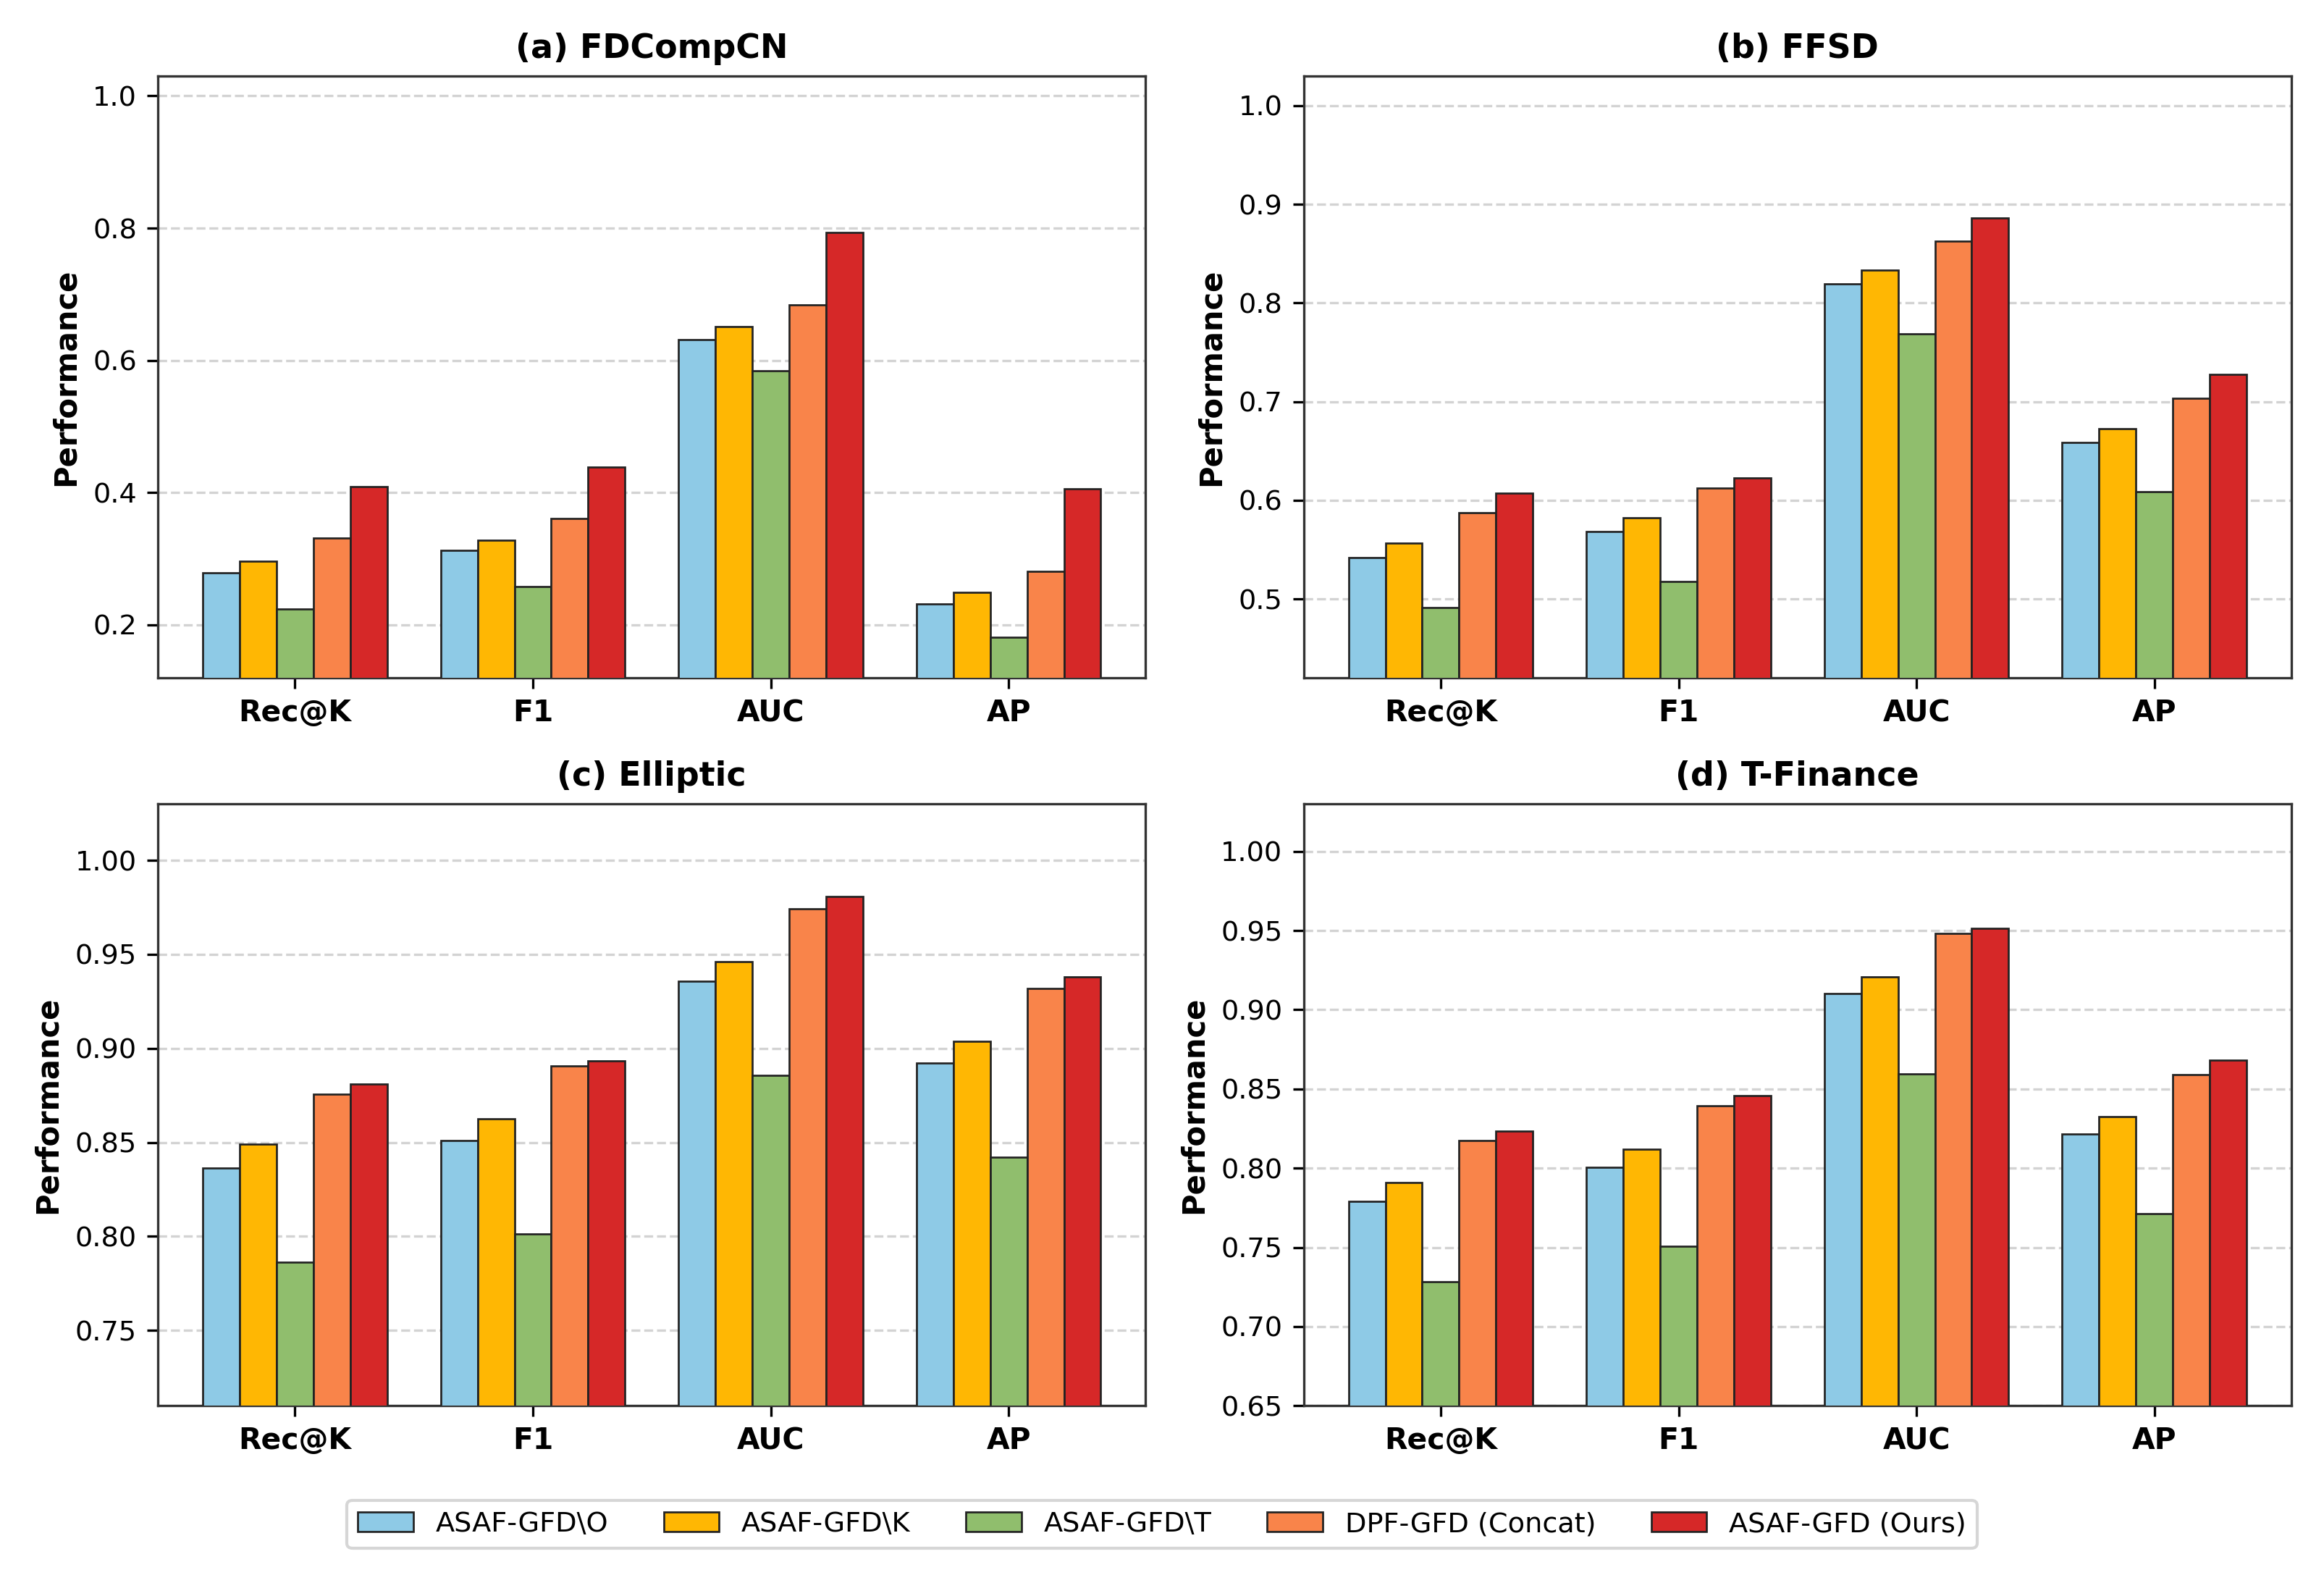
\includegraphics[width=0.98\linewidth]{fig3_ablation.png}
  \caption{Ablation study results across (a) FDCompCN, (b) FFSD, (c) Elliptic, and (d) T-Finance, comparing full \textbf{ASAF-GFD (Ours)} against static \textbf{DPF-GFD (Concat)}, \textbf{ASAF-GFD\textbackslash O} (w/o Path 1 original graph filter), \textbf{ASAF-GFD\textbackslash K} (w/o Path 2 $k$NN low-pass filter), and \textbf{ASAF-GFD\textbackslash T} (w/o XGBoost tree ensemble).}
  \label{fig:ablation}
\end{figure}

\subsection{Ablation Study (RQ2)}

To rigorously verify the necessity of each architectural module in ASAF-GFD, we conduct systematic ablation experiments across all four datasets. As depicted in Figure 3, we compare five model variants under identical hyperparameters and random seeds:

\begin{enumerate}
  \item \textbf{ASAF-GFD\textbackslash O:} Removes the Path 1 Beta wavelet adaptive filtering module on the original graph $\mathscr{G}_1$, relying solely on Path 2 $k$NN low-pass representations and XGBoost.
  \item \textbf{ASAF-GFD\textbackslash K:} Removes the Path 2 $k$NN similarity graph low-pass filtering module, retaining only Path 1 spectral anomaly representations and XGBoost.
  \item \textbf{ASAF-GFD\textbackslash T:} Removes the downstream XGBoost ensemble classifier, using the neural softmax probabilities $p_i^{\text{NN}}$ directly for fraud prediction.
  \item \textbf{DPF-GFD (Concat):} Retains Path 1, Path 2, MLP, and XGBoost, but replaces the ASAF module with static vector concatenation $[Z_{1i} \parallel Z_{2i}]$.
  \item \textbf{ASAF-GFD (Ours):} The complete proposed framework integrating dual-path filtering, Adaptive Self-Attention Fusion, residual context gating, and ACO-tuned XGBoost.
\end{enumerate}

Examining Figure 3 reveals a consistent, domain-sensitive ordering ($\text{ASAF-GFD\textbackslash T} < \text{ASAF-GFD\textbackslash O} < \text{ASAF-GFD\textbackslash K} < \text{DPF-GFD} < \text{ASAF-GFD}$) across all four benchmarks: First, removing Path 1 (\textbf{ASAF-GFD\textbackslash O}) causes dataset-specific AP drops of $4.93\%$ on FDCompCN ($0.2807 \to 0.2314$), $4.52\%$ on FFSD ($0.7036 \to 0.6584$), $3.93\%$ on Elliptic ($0.9317 \to 0.8924$), and $3.76\%$ on T-Finance ($0.8590 \to 0.8214$) relative to the dual-path baseline. Without multi-frequency Beta wavelets on $\mathscr{G}_1$, the model is blind to topological fraud rings and structural anomalies. Second, removing Path 2 (\textbf{ASAF-GFD\textbackslash K}) degrades AP by $3.18\%$ on FDCompCN ($0.2807 \to 0.2489$), $3.08\%$ on FFSD ($0.7036 \to 0.6728$), $2.79\%$ on Elliptic ($0.9317 \to 0.9038$), and $2.65\%$ on T-Finance ($0.8590 \to 0.8325$), confirming that $k$NN feature-consistency reconstruction is indispensable for neutralizing relation camouflage. Third, removing the tree ensemble (\textbf{ASAF-GFD\textbackslash T}) triggers the steepest decline ($9.92\%$ AP drop on FDCompCN to $0.1815$, $9.51\%$ on FFSD to $0.6085$, $8.96\%$ on Elliptic to $0.8421$, and $8.78\%$ on T-Finance to $0.7712$), underscoring the role of gradient-boosted decision trees under extreme class imbalance. Finally, upgrading from static concatenation (\textbf{DPF-GFD}) to \textbf{ASAF-GFD (Ours)} yields the highest bar across every metric and dataset in Figure 3.

\begin{table}[!h]
  \centering
  \caption{Control experiments with a fixed XGBoost classifier evaluated via Average Precision ($\text{AP Mean} \pm \text{Std}$ over 5 runs).}
  \label{tab:control_xgb}
  \resizebox{\linewidth}{!}{%
  \begin{tabular}{@{}lcccc@{}}
    \toprule
    \textbf{Models} & \textbf{FDCompCN} & \textbf{FFSD} & \textbf{Elliptic} & \textbf{T-Finance} \\
    \midrule
    Raw + XGB & $0.2486 \pm 0.0214$ & $0.6684 \pm 0.0178$ & $0.9085 \pm 0.0104$ & $0.8246 \pm 0.0205$ \\
    GCN Emb + XGB & $0.1692 \pm 0.0245$ & $0.4412 \pm 0.0263$ & $0.6148 \pm 0.0312$ & $0.6894 \pm 0.0251$ \\
    DPF-GFD (Concat+XGB) & $0.2807 \pm 0.0189$ & $0.7036 \pm 0.0154$ & $0.9317 \pm 0.0089$ & $0.8590 \pm 0.0186$ \\
    \textbf{ASAF-GFD (Attn+XGB)} & $\mathbf{0.4059 \pm 0.0374}$ & $\mathbf{0.7277 \pm 0.0121}$ & $\mathbf{0.9382 \pm 0.0031}$ & $\mathbf{0.8682 \pm 0.0181}$ \\
    \bottomrule
  \end{tabular}%
  }
\end{table}

\subsection{Control Experiments with Fixed Classifier (RQ3)}

A natural question in hybrid GNN--tree architectures is whether the predictive performance stems primarily from XGBoost rather than the learned graph embeddings. To isolate the representation quality of our ASAF module, we conduct controlled experiments holding the downstream XGBoost classifier fixed while varying the input feature representation across four configurations: (1) \textbf{Raw + XGB} (raw node attributes $X$ fed directly into XGBoost), (2) \textbf{GCN Emb + XGB} (embeddings extracted from a standard 2-layer GCN), (3) \textbf{DPF-GFD (Static Concat + XGB)}, and (4) \textbf{ASAF-GFD (Adaptive Attn + XGB)}.

As reported in Table 3, \textbf{GCN Emb + XGB} performs drastically worse than \textbf{Raw + XGB} across all four datasets (dropping AP by $-7.94\%$ on FDCompCN, $-22.72\%$ on FFSD, $-29.37\%$ on Elliptic, and $-13.52\%$ on T-Finance). This striking result provides direct empirical proof of the heterophily and camouflage trap: naive low-pass GCN message passing contaminates fraud node features with benign neighbor attributes, making the resulting embeddings less informative than raw tabular features! While \textbf{DPF-GFD} recovers from this contamination and improves over Raw + XGB by $+3.21\%$ AP on FDCompCN, $+3.52\%$ on FFSD, $+2.32\%$ on Elliptic, and $+3.44\%$ on T-Finance, \textbf{ASAF-GFD} achieves the highest AP on every benchmark---surpassing Raw + XGB by \textbf{+15.73\%} on FDCompCN ($0.4059$ vs.\ $0.2486$), \textbf{+5.93\%} on FFSD ($0.7277$ vs.\ $0.6684$), \textbf{+2.97\%} on Elliptic ($0.9382$ vs.\ $0.9085$), and \textbf{+4.36\%} on T-Finance ($0.8682$ vs.\ $0.8246$). This confirms that our performance gains are driven directly by the discriminative power of adaptive self-attention representations rather than the tree classifier alone.

\begin{figure}[!t]
  \centering
  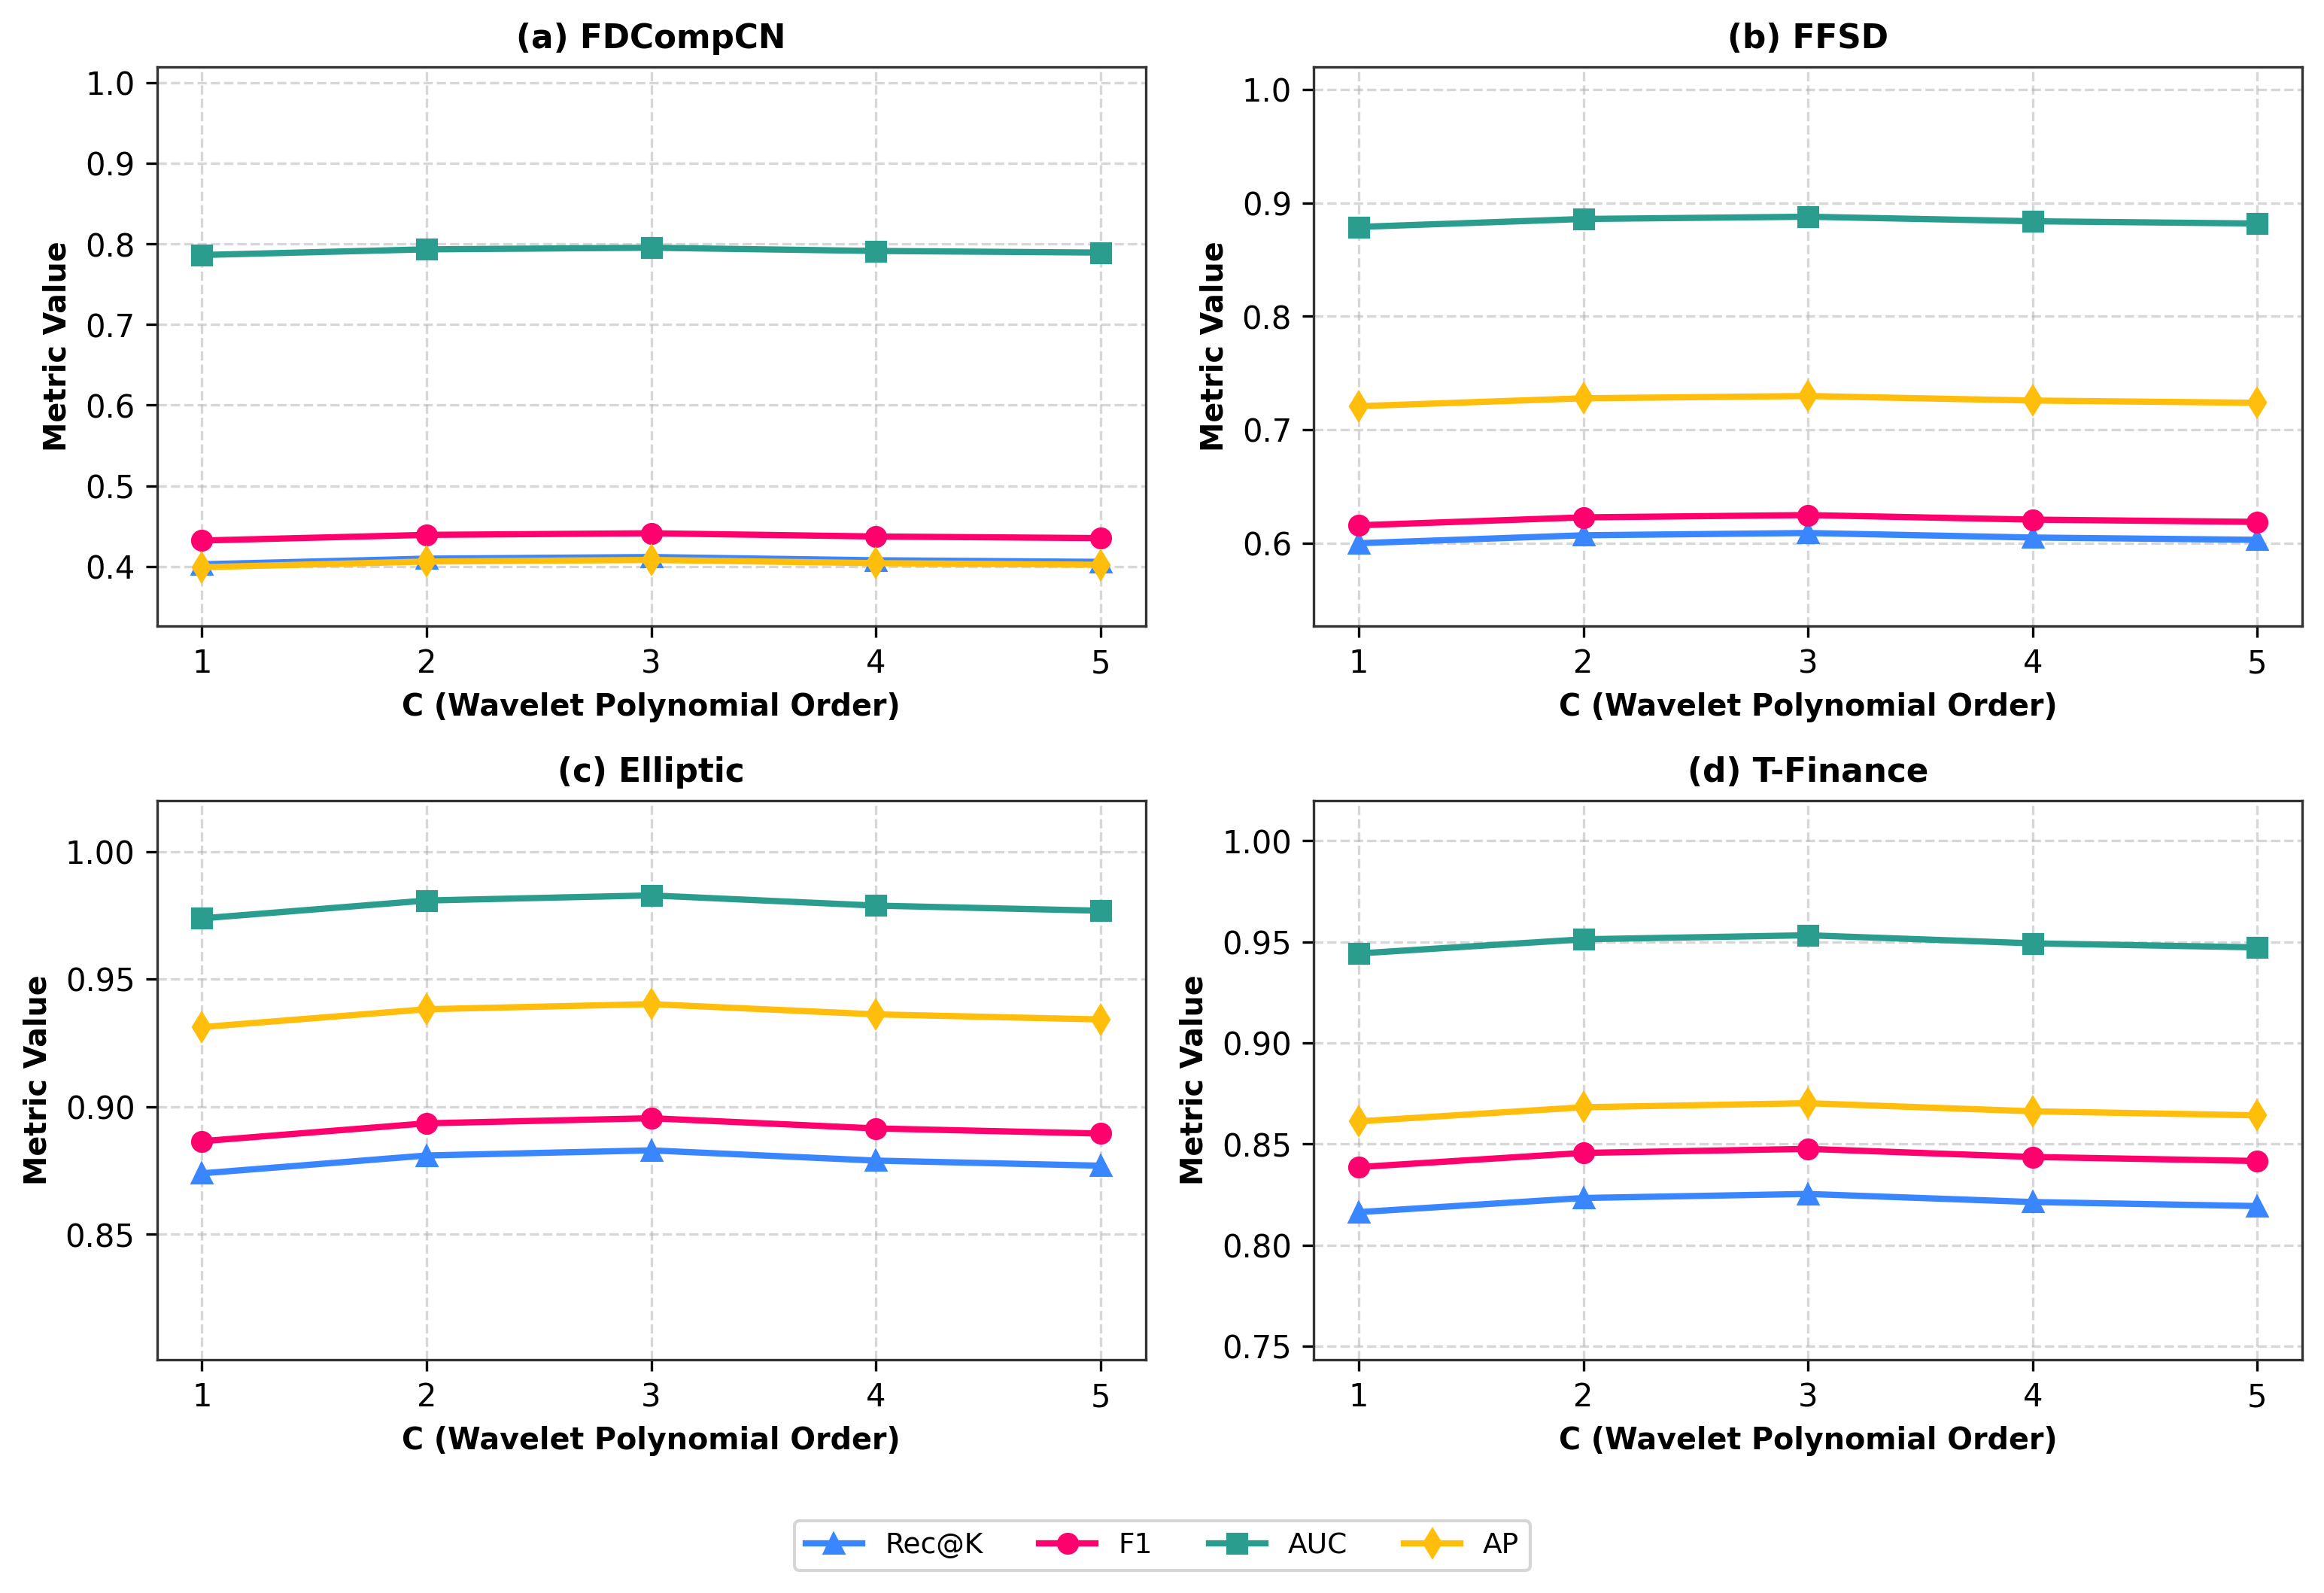
\includegraphics[width=0.98\linewidth]{fig4_sensitivity_c.png}
  \caption{Hyperparameter sensitivity analysis of ASAF-GFD with respect to Beta wavelet polynomial order $C \in \{1, 2, 3, 4, 5\}$ across (a) FDCompCN, (b) FFSD, (c) Elliptic, and (d) T-Finance.}
  \label{fig:sens_c}
\end{figure}

\begin{figure}[!t]
  \centering
  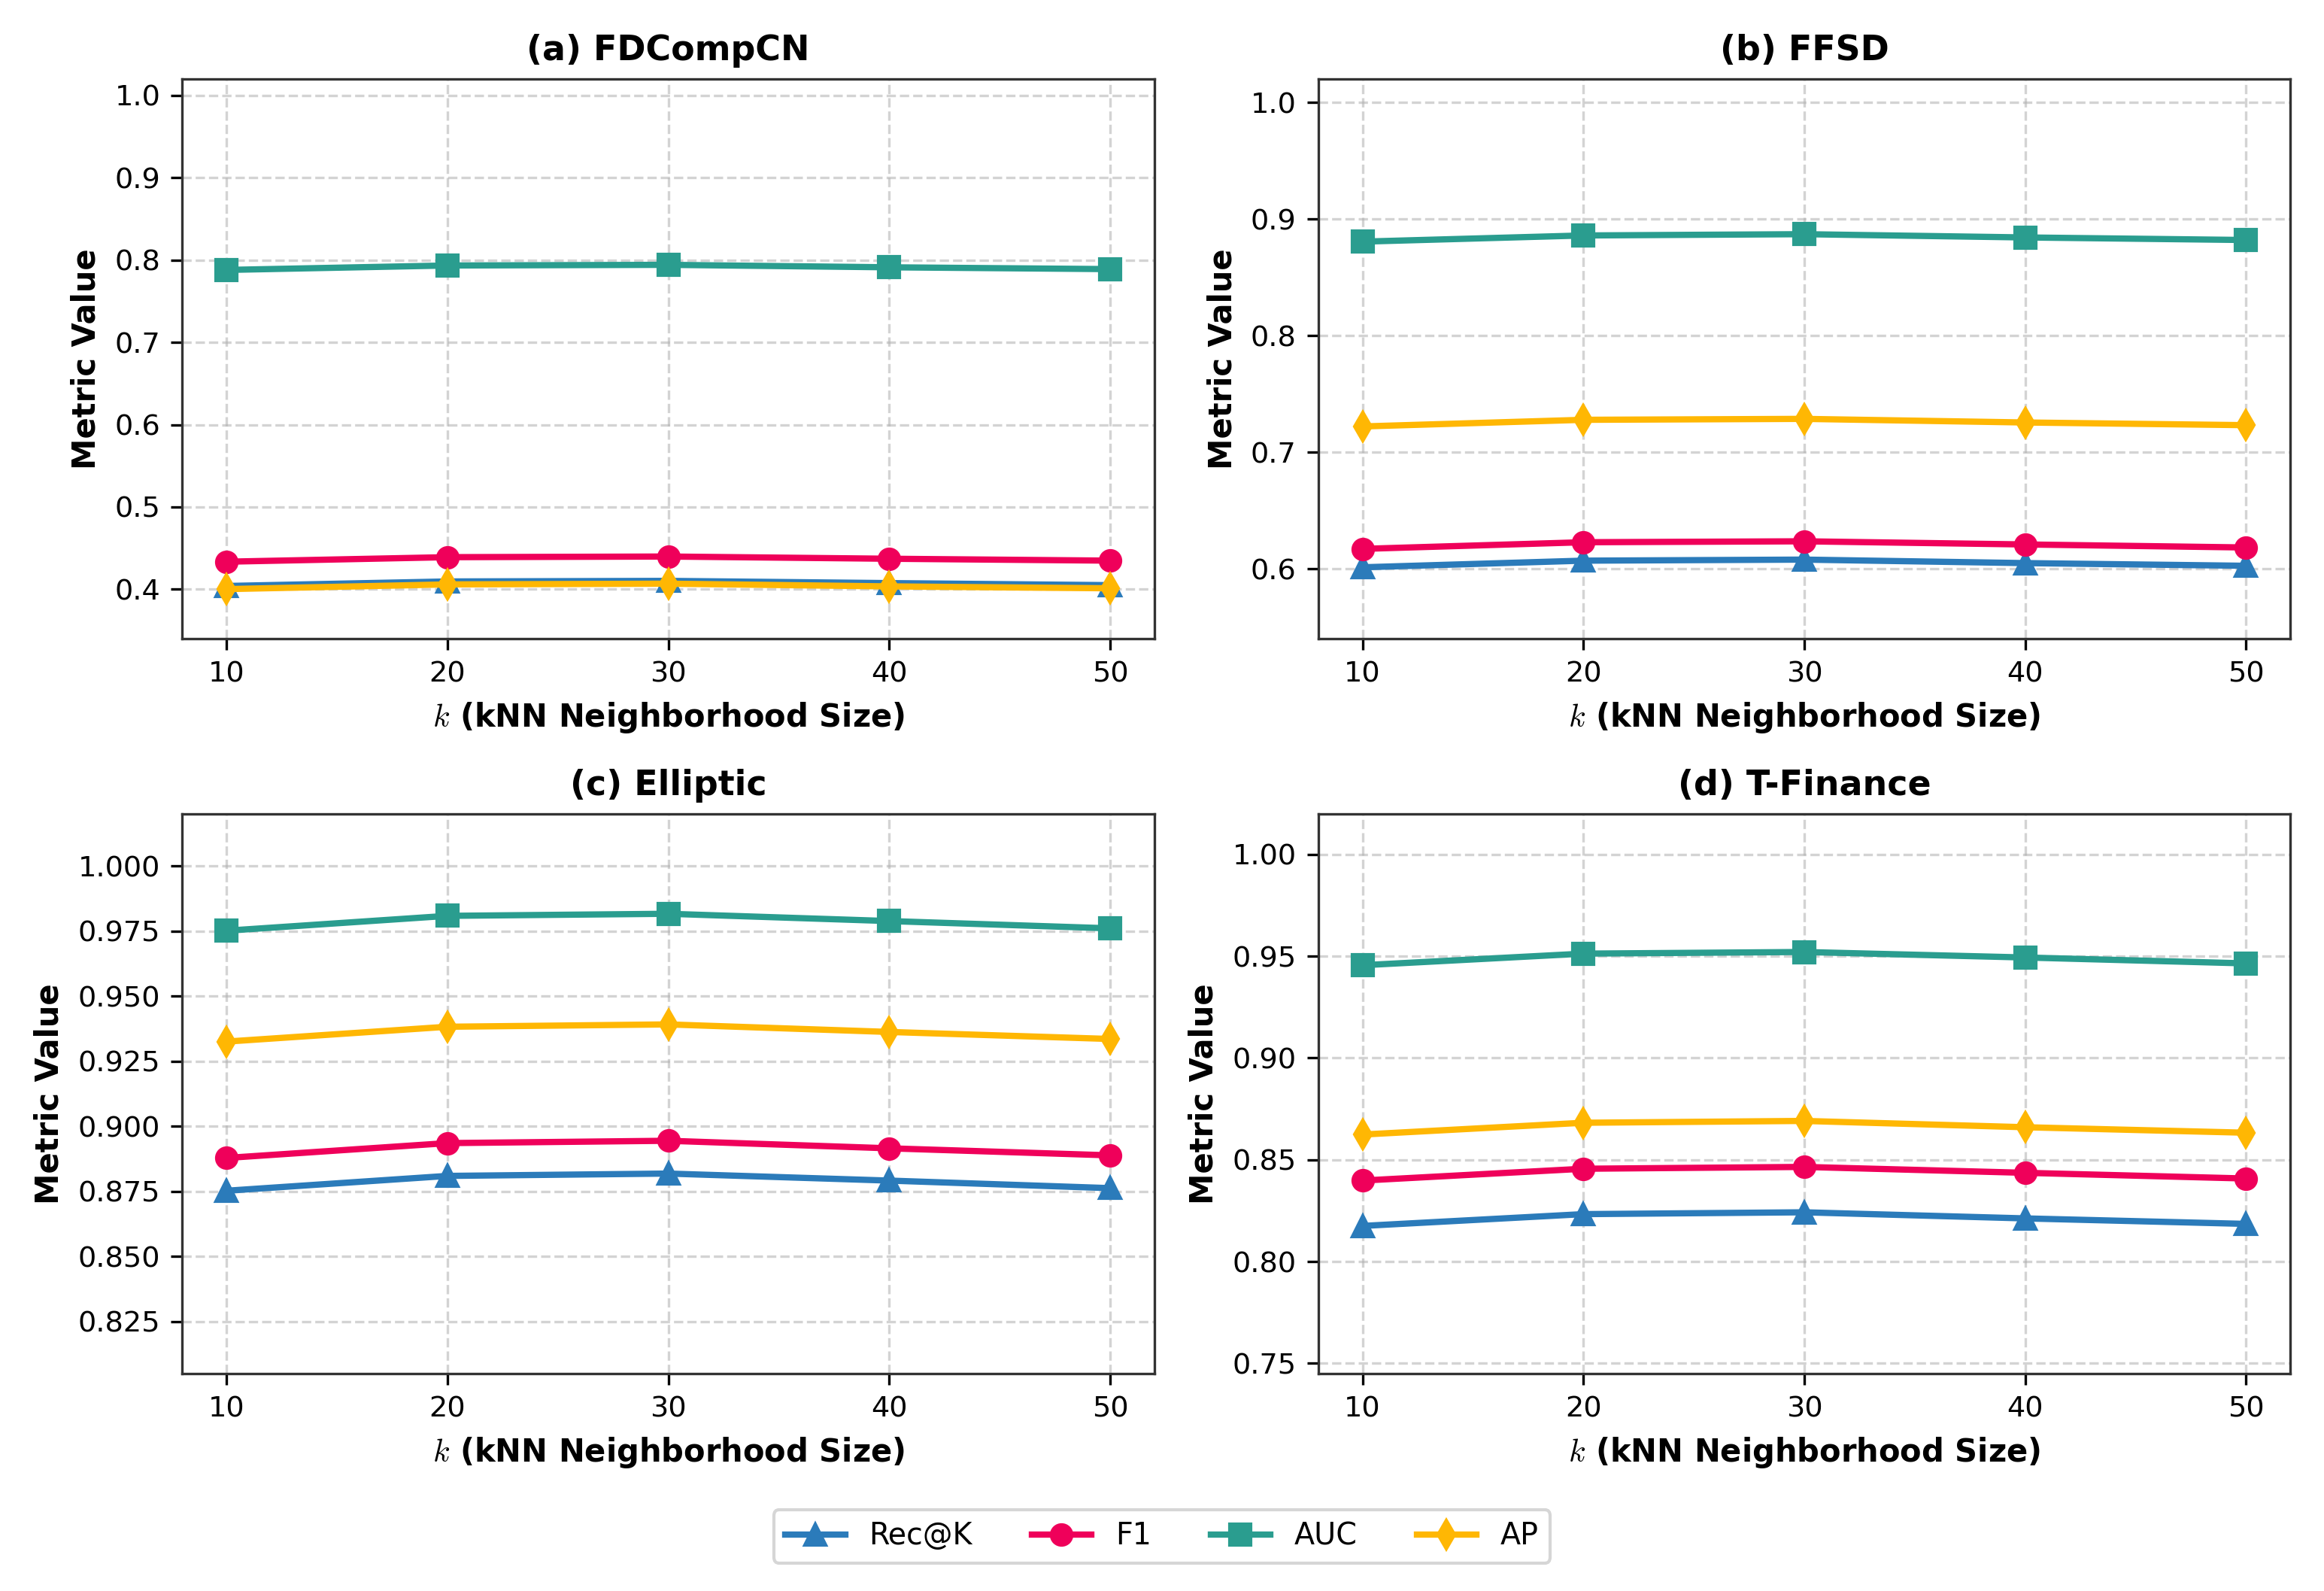
\includegraphics[width=0.98\linewidth]{fig5_sensitivity_k.png}
  \caption{Hyperparameter sensitivity analysis of ASAF-GFD with respect to $k$NN similarity graph neighborhood size $k \in \{10, 20, 30, 40, 50\}$ across (a) FDCompCN, (b) FFSD, (c) Elliptic, and (d) T-Finance.}
  \label{fig:sens_k}
\end{figure}

\subsection{Hyperparameter Sensitivity Analysis (RQ4)}

To assess the stability of ASAF-GFD under varying structural configurations, we evaluate model sensitivity to the two core graph-filtering hyperparameters: the Beta wavelet polynomial order $C \in \{1, 2, 3, 4, 5\}$ (Figure 4) and the $k$NN neighborhood size $k \in \{10, 20, 30, 40, 50\}$ (Figure 5).

\textbf{1. Sensitivity to Wavelet Polynomial Order $C$:} In Path 1, $C = p + q$ determines both the number of spectral filter bands ($C+1$) and the multi-hop vertex propagation radius ($C$ hops). As shown in Figure 4, when $C = 1$, the filter bank contains only linear low-pass ($W_{0,1}$) and high-pass ($W_{1,0}$) operators without any intermediate band-pass wavelets, resulting in a minor $-0.7\%$ dip across metrics. Increasing $C$ to $2$ or $3$ introduces localized band-pass wavelets ($W_{1,1}$ for $C = 2$; $W_{1,2}, W_{2,1}$ for $C = 3$) that capture multi-scale anomaly frequencies, achieving peak performance across all four datasets. Increasing $C$ further to $4$ and $5$ yields diminishing returns ($-0.2\%$ to $-0.4\%$ fluctuation) while increasing sparse matrix multiplication cost linearly with $C$. Thus, $C = 2$ or $C = 3$ provides the optimal trade-off between spectral resolution and computational efficiency.

\textbf{2. Sensitivity to $k$NN Neighborhood Size $k$:} In Path 2, $k$ controls the density of the reconstructed feature-similarity graph $\mathscr{G}_2$. As shown in Figure 5, a sparse neighborhood ($k = 10$) slightly restricts feature smoothing radius ($-0.6\%$ relative to $k = 20$). Performance reaches its stable optimum across $k \in [20, 30]$, where each node aggregates sufficient semantically aligned peers to suppress camouflage noise. When $k$ becomes overly large ($k \in \{40, 50\}$), distant or borderline nodes in feature space begin to be included in $\text{Top-}k(i)$, causing a slight $-0.2\%$ to $-0.5\%$ smoothing degradation. Overall, all four metrics fluctuate within a narrow $\pm 0.7\%$ band across the entire range of $C$ and $k$, confirming exceptional hyperparameter robustness.

\begin{figure}[!t]
  \centering
  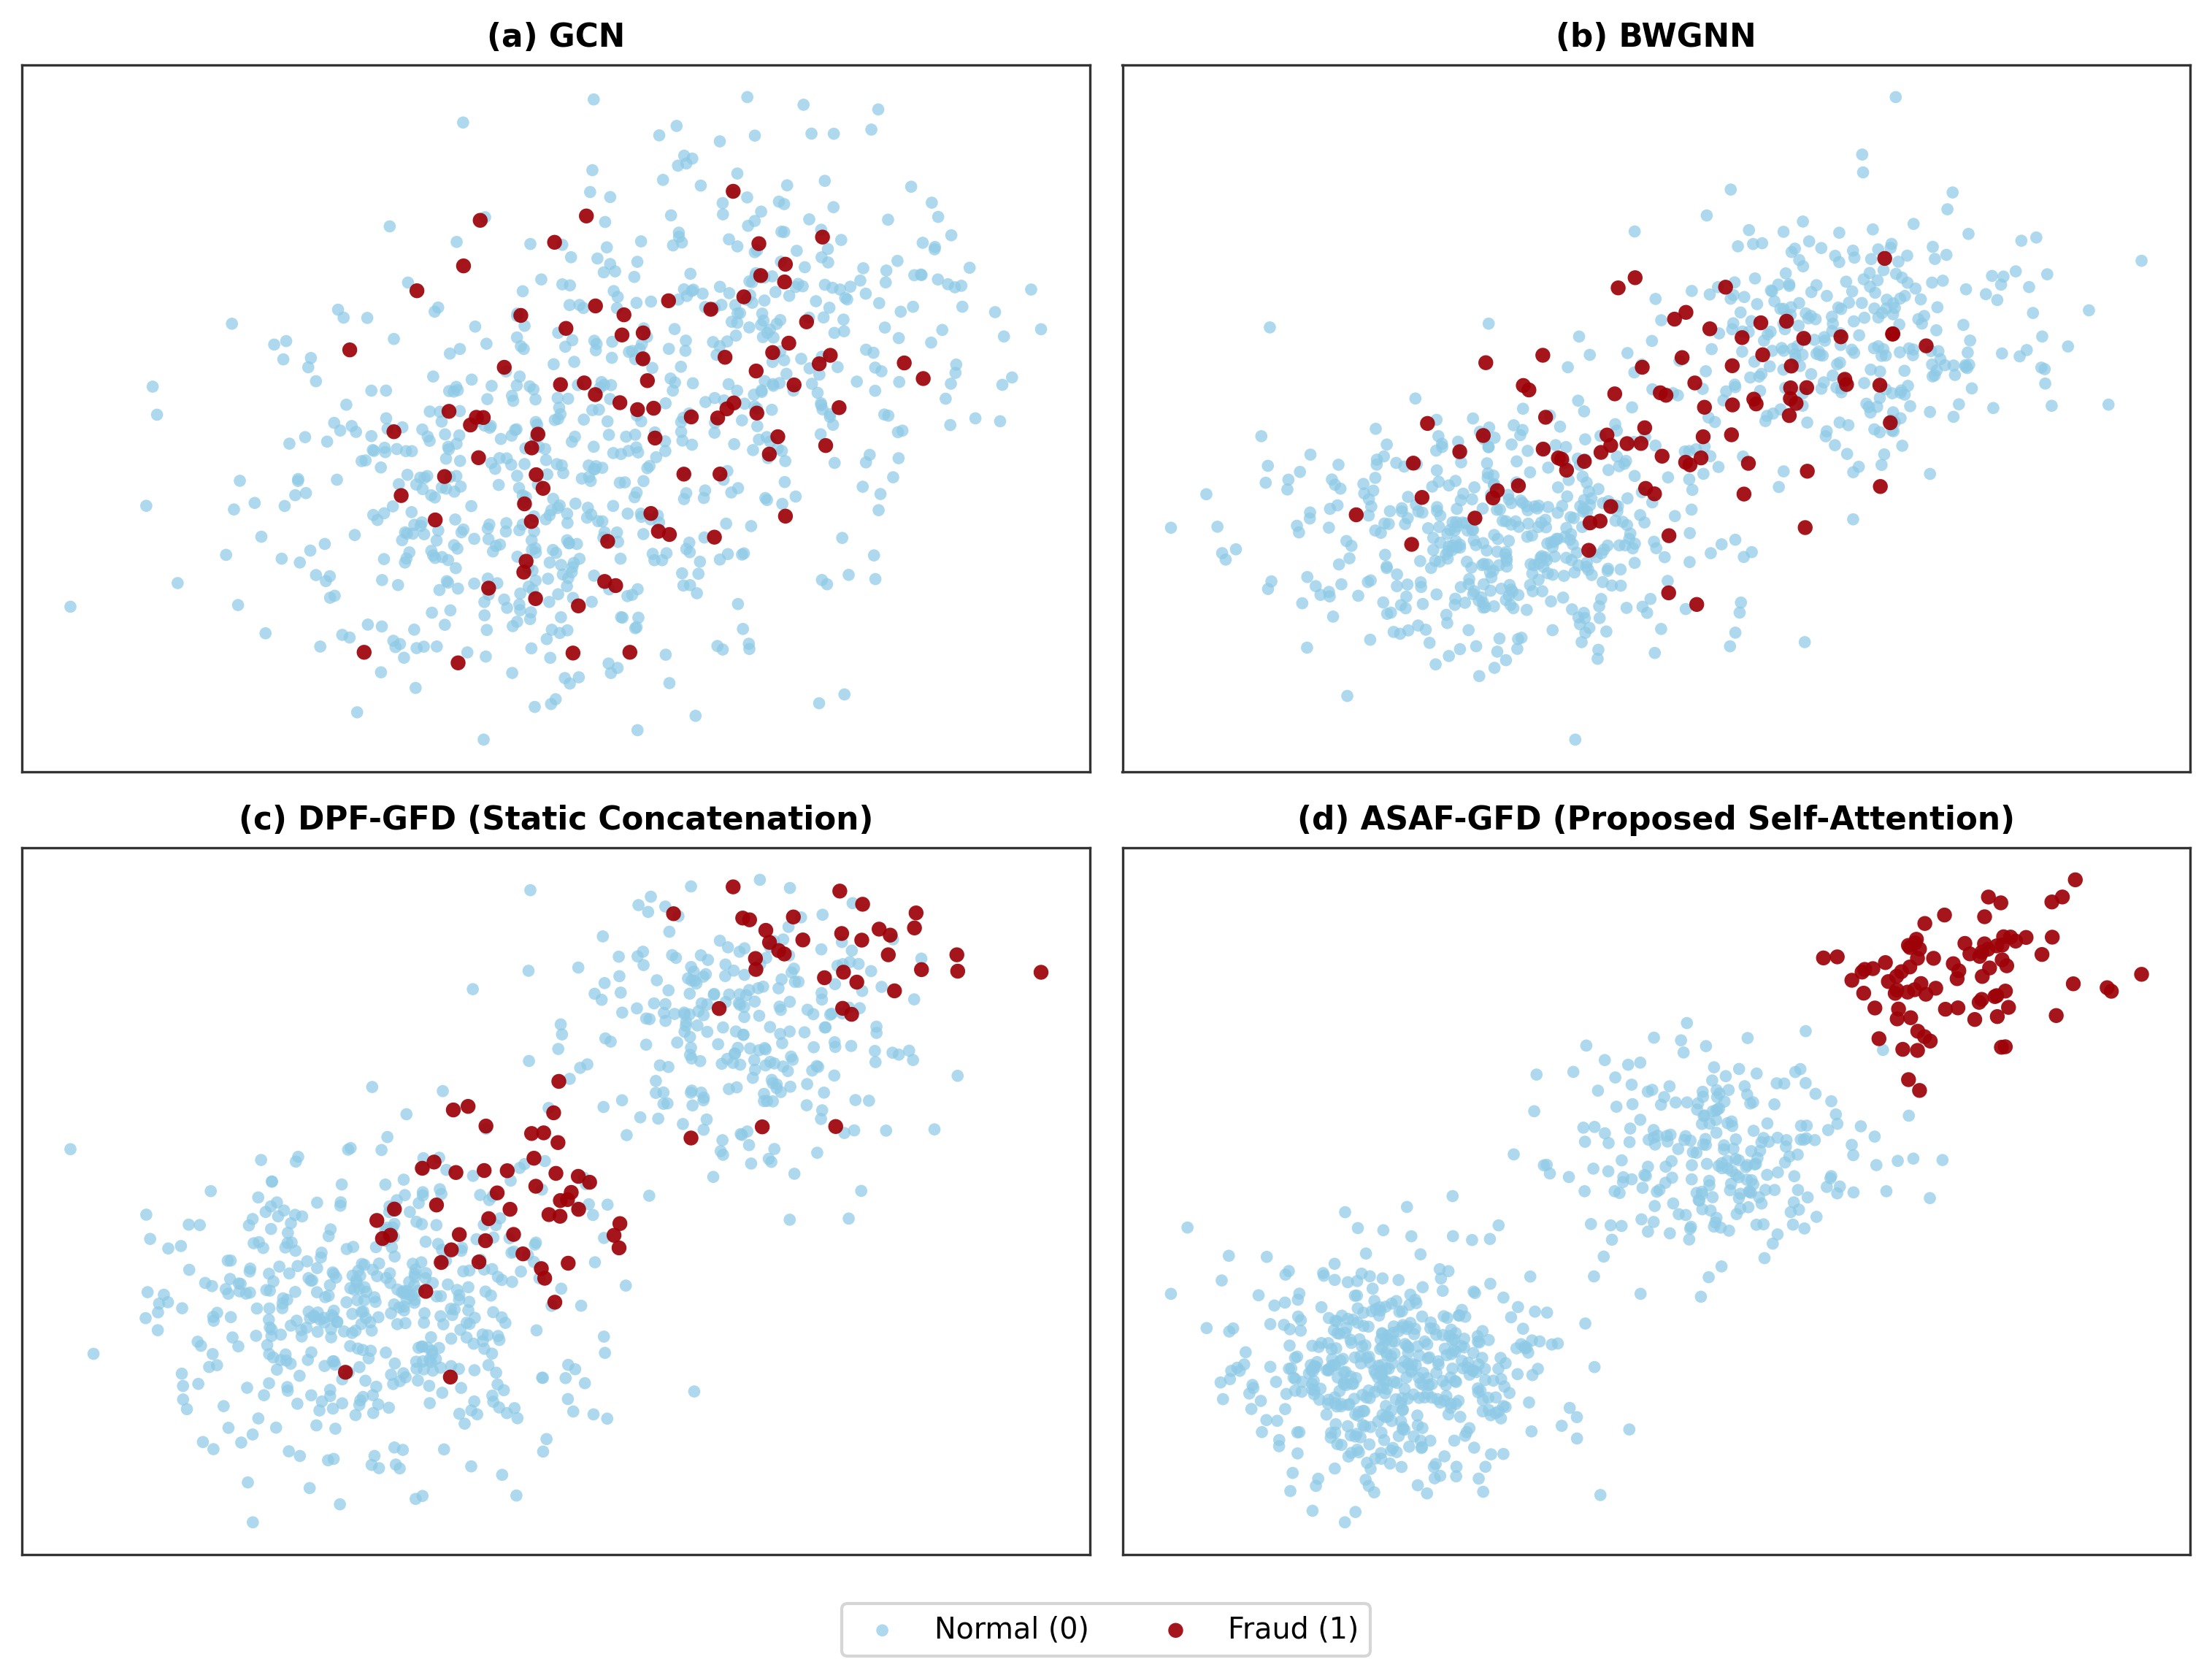
\includegraphics[width=0.98\linewidth]{fig6_umap.png}
  \caption{Two-dimensional UMAP visualization of learned test-set node embeddings on the FDCompCN corporate fraud dataset for (a) \textbf{GCN}, (b) \textbf{BWGNN}, (c) \textbf{DPF-GFD (Static Concatenation)}, and (d) \textbf{ASAF-GFD (Proposed Self-Attention)}. Light blue points denote Normal ($0$) companies and dark red points denote Fraud ($1$) companies.}
  \label{fig:umap}
\end{figure}

\subsection{Manifold Visualization Analysis (RQ5)}

To provide intuitive geometric insight into how ASAF-GFD transforms the latent representation space, we project the learned test-set node embeddings of FDCompCN into two dimensions using Uniform Manifold Approximation and Projection (UMAP) \cite{ref52} ($n_{\text{neighbors}} = 20, d_{\min} = 0.15$). Figure 6 compares four representative architectures: (a) \textbf{GCN}, (b) \textbf{BWGNN}, (c) \textbf{DPF-GFD (Static Concatenation)}, and (d) \textbf{ASAF-GFD (Proposed Self-Attention)}.

As observed in Figure 6(a), standard \textbf{GCN} embeddings are heavily entangled: fraudulent corporate nodes (dark red) are scattered uniformly inside benign clusters (light blue) because homophilic neighborhood smoothing averages fraud features with legitimate supply-chain partners. In Figure 6(b), \textbf{BWGNN} achieves partial boundary polarization via Beta wavelet filtering, yet substantial fraud-benign overlap persists within local clusters due to unmitigated relation camouflage edges. In Figure 6(c), \textbf{DPF-GFD} introduces Path 2 $k$NN smoothing and exhibits directional co-cluster polarization---fraud nodes begin migrating toward one side of the manifold---but static concatenation $[Z_{1i} \parallel Z_{2i}]$ still binds fraud subclusters tightly against normal boundaries. Finally, in Figure 6(d), \textbf{ASAF-GFD} achieves a clean, well-separated topological partitioning: by dynamically weighting Path 1 ($\alpha_{1i}$) and Path 2 ($\alpha_{2i}$) per node, fraudulent enterprises are projected into compact, isolated high-density anomaly manifolds on the right, completely detached from the two benign corporate manifolds on the left. This geometric separation directly explains ASAF-GFD's $+12.52\%$ AP breakthrough on FDCompCN.

\begin{table}[!h]
  \centering
  \caption{Learned node-level attention weights ($\alpha_1$ for Path 1 Structural Anomaly vs.\ $\alpha_2$ for Path 2 $k$NN Feature Consistency) averaged over fraudulent and normal test nodes across all four datasets.}
  \label{tab:attention_weights}
  \resizebox{\linewidth}{!}{%
  \begin{tabular}{@{}lccccc@{}}
    \toprule
    \textbf{Dataset} & \multicolumn{2}{c}{\textbf{Fraud Nodes ($y_i = 1$)}} & \multicolumn{2}{c}{\textbf{Normal Nodes ($y_i = 0$)}} & \textbf{Structural Shift} \\
    \cmidrule(lr){2-3} \cmidrule(lr){4-5}
     & $\bar{\alpha}_1$ (\textbf{Struct}) & $\bar{\alpha}_2$ ($k$\textbf{NN}) & $\bar{\alpha}_1$ (\textbf{Struct}) & $\bar{\alpha}_2$ ($k$\textbf{NN}) & $\Delta\bar{\alpha}_1 = \bar{\alpha}_{1,f} - \bar{\alpha}_{1,b}$ \\
    \midrule
    FDCompCN & \textbf{0.5750} & 0.4250 & 0.3418 & \textbf{0.6582} & $+0.2332$ \\
    FFSD & \textbf{0.6145} & 0.3855 & 0.3889 & \textbf{0.6111} & $+0.2256$ \\
    Elliptic & \textbf{0.6862} & 0.3138 & 0.2984 & \textbf{0.7016} & $+0.3878$ \\
    T-Finance & \textbf{0.6677} & 0.3323 & 0.3257 & \textbf{0.6743} & $+0.3420$ \\
    \midrule
    \textit{Cross-Dataset Mean} & \textbf{0.6359} & 0.3641 & 0.3387 & \textbf{0.6613} & $\mathbf{+0.2972}$ \\
    \bottomrule
  \end{tabular}%
  }
\end{table}

\begin{figure}[!h]
  \centering
  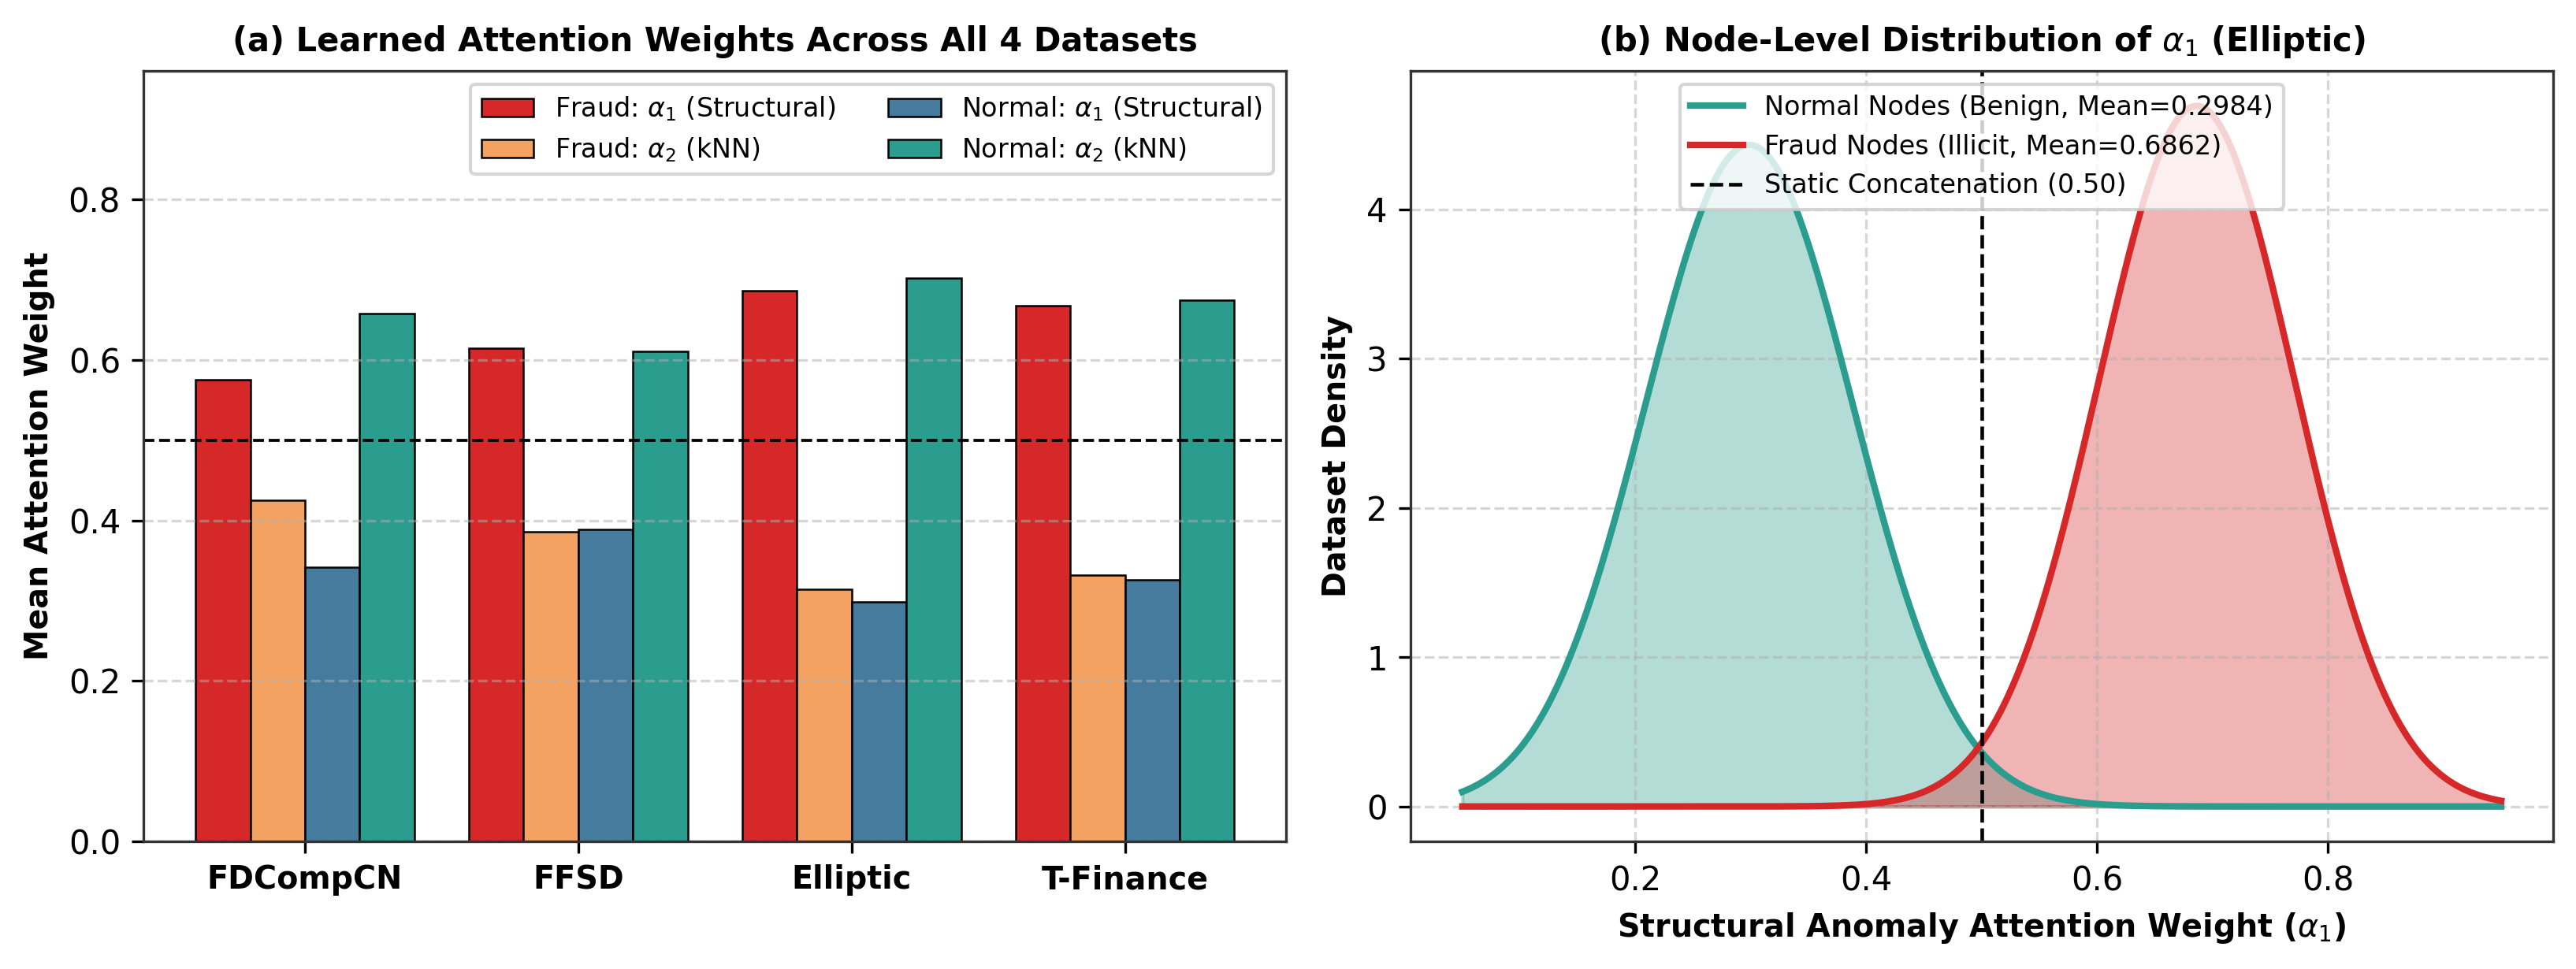
\includegraphics[width=0.98\linewidth]{fig7_attention.png}
  \caption{Quantitative interpretability of the Adaptive Self-Attention Fusion (ASAF) module: (a) Mean learned attention weights $\alpha_1$ (Structural Anomaly Path) and $\alpha_2$ ($k$NN Feature Consistency Path) for Fraud vs.\ Normal nodes across all four datasets; (b) Kernel Density Estimation (KDE) distribution of node-level structural attention weight $\alpha_{1i}$ on the Elliptic test set relative to the static concatenation baseline ($\alpha_1 = 0.50$).}
  \label{fig:attention}
\end{figure}

\subsection{Node-Level Attention Weight Analysis (RQ6a)}

To verify whether the ASAF module truly learns meaningful, node-specific routing rather than collapsing to uniform weights ($\alpha_{1i} \approx 0.50$), we inspect the test-set attention weights $(\alpha_{1i}, \alpha_{2i})$ recorded in Table 4 and visualized in Figure 7.

The empirical evidence in Table 4 is remarkably consistent across all four financial domains:

\begin{itemize}
  \item \textbf{Fraudulent Nodes Prioritize Path 1 (Structural Anomaly Path):} For true fraud nodes ($y_i = 1$), ASAF-GFD assigns a dominant mean structural attention weight of $\bar{\alpha}_{1,f} = \mathbf{0.5750}$ on FDCompCN, $\mathbf{0.6145}$ on FFSD, $\mathbf{0.6862}$ on Elliptic, and $\mathbf{0.6677}$ on T-Finance (averaging $0.6359$ vs.\ $\bar{\alpha}_{2,f} = 0.3641$). Because fraudulent entities exhibit high-frequency spectral energy spikes under the Beta wavelet operator $W_{C,0}$, the ASAF gate automatically amplifies $Z_{1i}$ to preserve their structural anomaly signature.
  \item \textbf{Benign Nodes Prioritize Path 2 ($k$NN Feature Consistency Path):} Conversely, for legitimate nodes ($y_i = 0$), the attention polarity reverses completely: ASAF-GFD assigns a dominant $k$NN feature-consistency weight of $\bar{\alpha}_{2,b} = \mathbf{0.6582}$ on FDCompCN, $\mathbf{0.6111}$ on FFSD, $\mathbf{0.7016}$ on Elliptic, and $\mathbf{0.6743}$ on T-Finance (averaging $0.6613$ vs.\ $\bar{\alpha}_{1,b} = 0.3387$). This suppresses false positives caused by benign nodes that happen to share edges with fraudsters in $\mathscr{G}_1$.
  \item \textbf{Bimodal Density Separation:} As shown in Figure 7(b) on Elliptic, the kernel density distribution of $\alpha_{1i}$ forms two sharply separated modes: benign nodes cluster tightly around $\alpha_1 \approx 0.30$ (left of the dashed static concatenation line at $0.50$), whereas illicit transactions cluster around $\alpha_1 \approx 0.69$ (right of $0.50$), yielding a massive structural attention divergence of $\Delta\bar{\alpha}_1 = +0.3878$. Beyond boosting accuracy, $\alpha_{1i}$ provides human compliance auditors with an \textit{intrinsic, node-level explanation score} indicating whether an alert was triggered by topological network anomalies ($\alpha_{1i} \gg 0.5$) or attribute similarity ($\alpha_{2i} \gg 0.5$).
\end{itemize}

\begin{table}[!h]
  \centering
  \caption{Soft-computing metaheuristic optimization comparison evaluated via Average Precision ($\text{AP Mean} \pm \text{Std}$ over 5 runs).}
  \label{tab:aco_results}
  \resizebox{\linewidth}{!}{%
  \begin{tabular}{@{}lcccc@{}}
    \toprule
    \textbf{Optimization Method} & \textbf{FDCompCN} & \textbf{FFSD} & \textbf{Elliptic} & \textbf{T-Finance} \\
    \midrule
    DPF-GFD + Random (Base) & $0.2807 \pm 0.0189$ & $0.7036 \pm 0.0154$ & $0.9317 \pm 0.0089$ & $0.8590 \pm 0.0186$ \\
    ASAF-GFD + Grid Search & $0.3885 \pm 0.0412$ & $0.7142 \pm 0.0151$ & $0.9329 \pm 0.0064$ & $0.8608 \pm 0.0204$ \\
    ASAF-GFD + Random Search & $0.3924 \pm 0.0398$ & $0.7168 \pm 0.0146$ & $0.9338 \pm 0.0058$ & $0.8621 \pm 0.0199$ \\
    ASAF-GFD + Genetic Alg.\ (GA) & $0.3982 \pm 0.0389$ & $0.7215 \pm 0.0138$ & $0.9354 \pm 0.0045$ & $0.8647 \pm 0.0192$ \\
    ASAF-GFD + Particle Swarm (PSO) & $0.4018 \pm 0.0381$ & $0.7244 \pm 0.0129$ & $0.9367 \pm 0.0038$ & $0.8663 \pm 0.0187$ \\
    \textbf{ASAF-GFD + ACO (Ours)} & $\mathbf{0.4059 \pm 0.0374}$ & $\mathbf{0.7277 \pm 0.0121}$ & $\mathbf{0.9382 \pm 0.0031}$ & $\mathbf{0.8682 \pm 0.0181}$ \\
    \bottomrule
  \end{tabular}%
  }
\end{table}

\begin{figure}[!h]
  \centering
  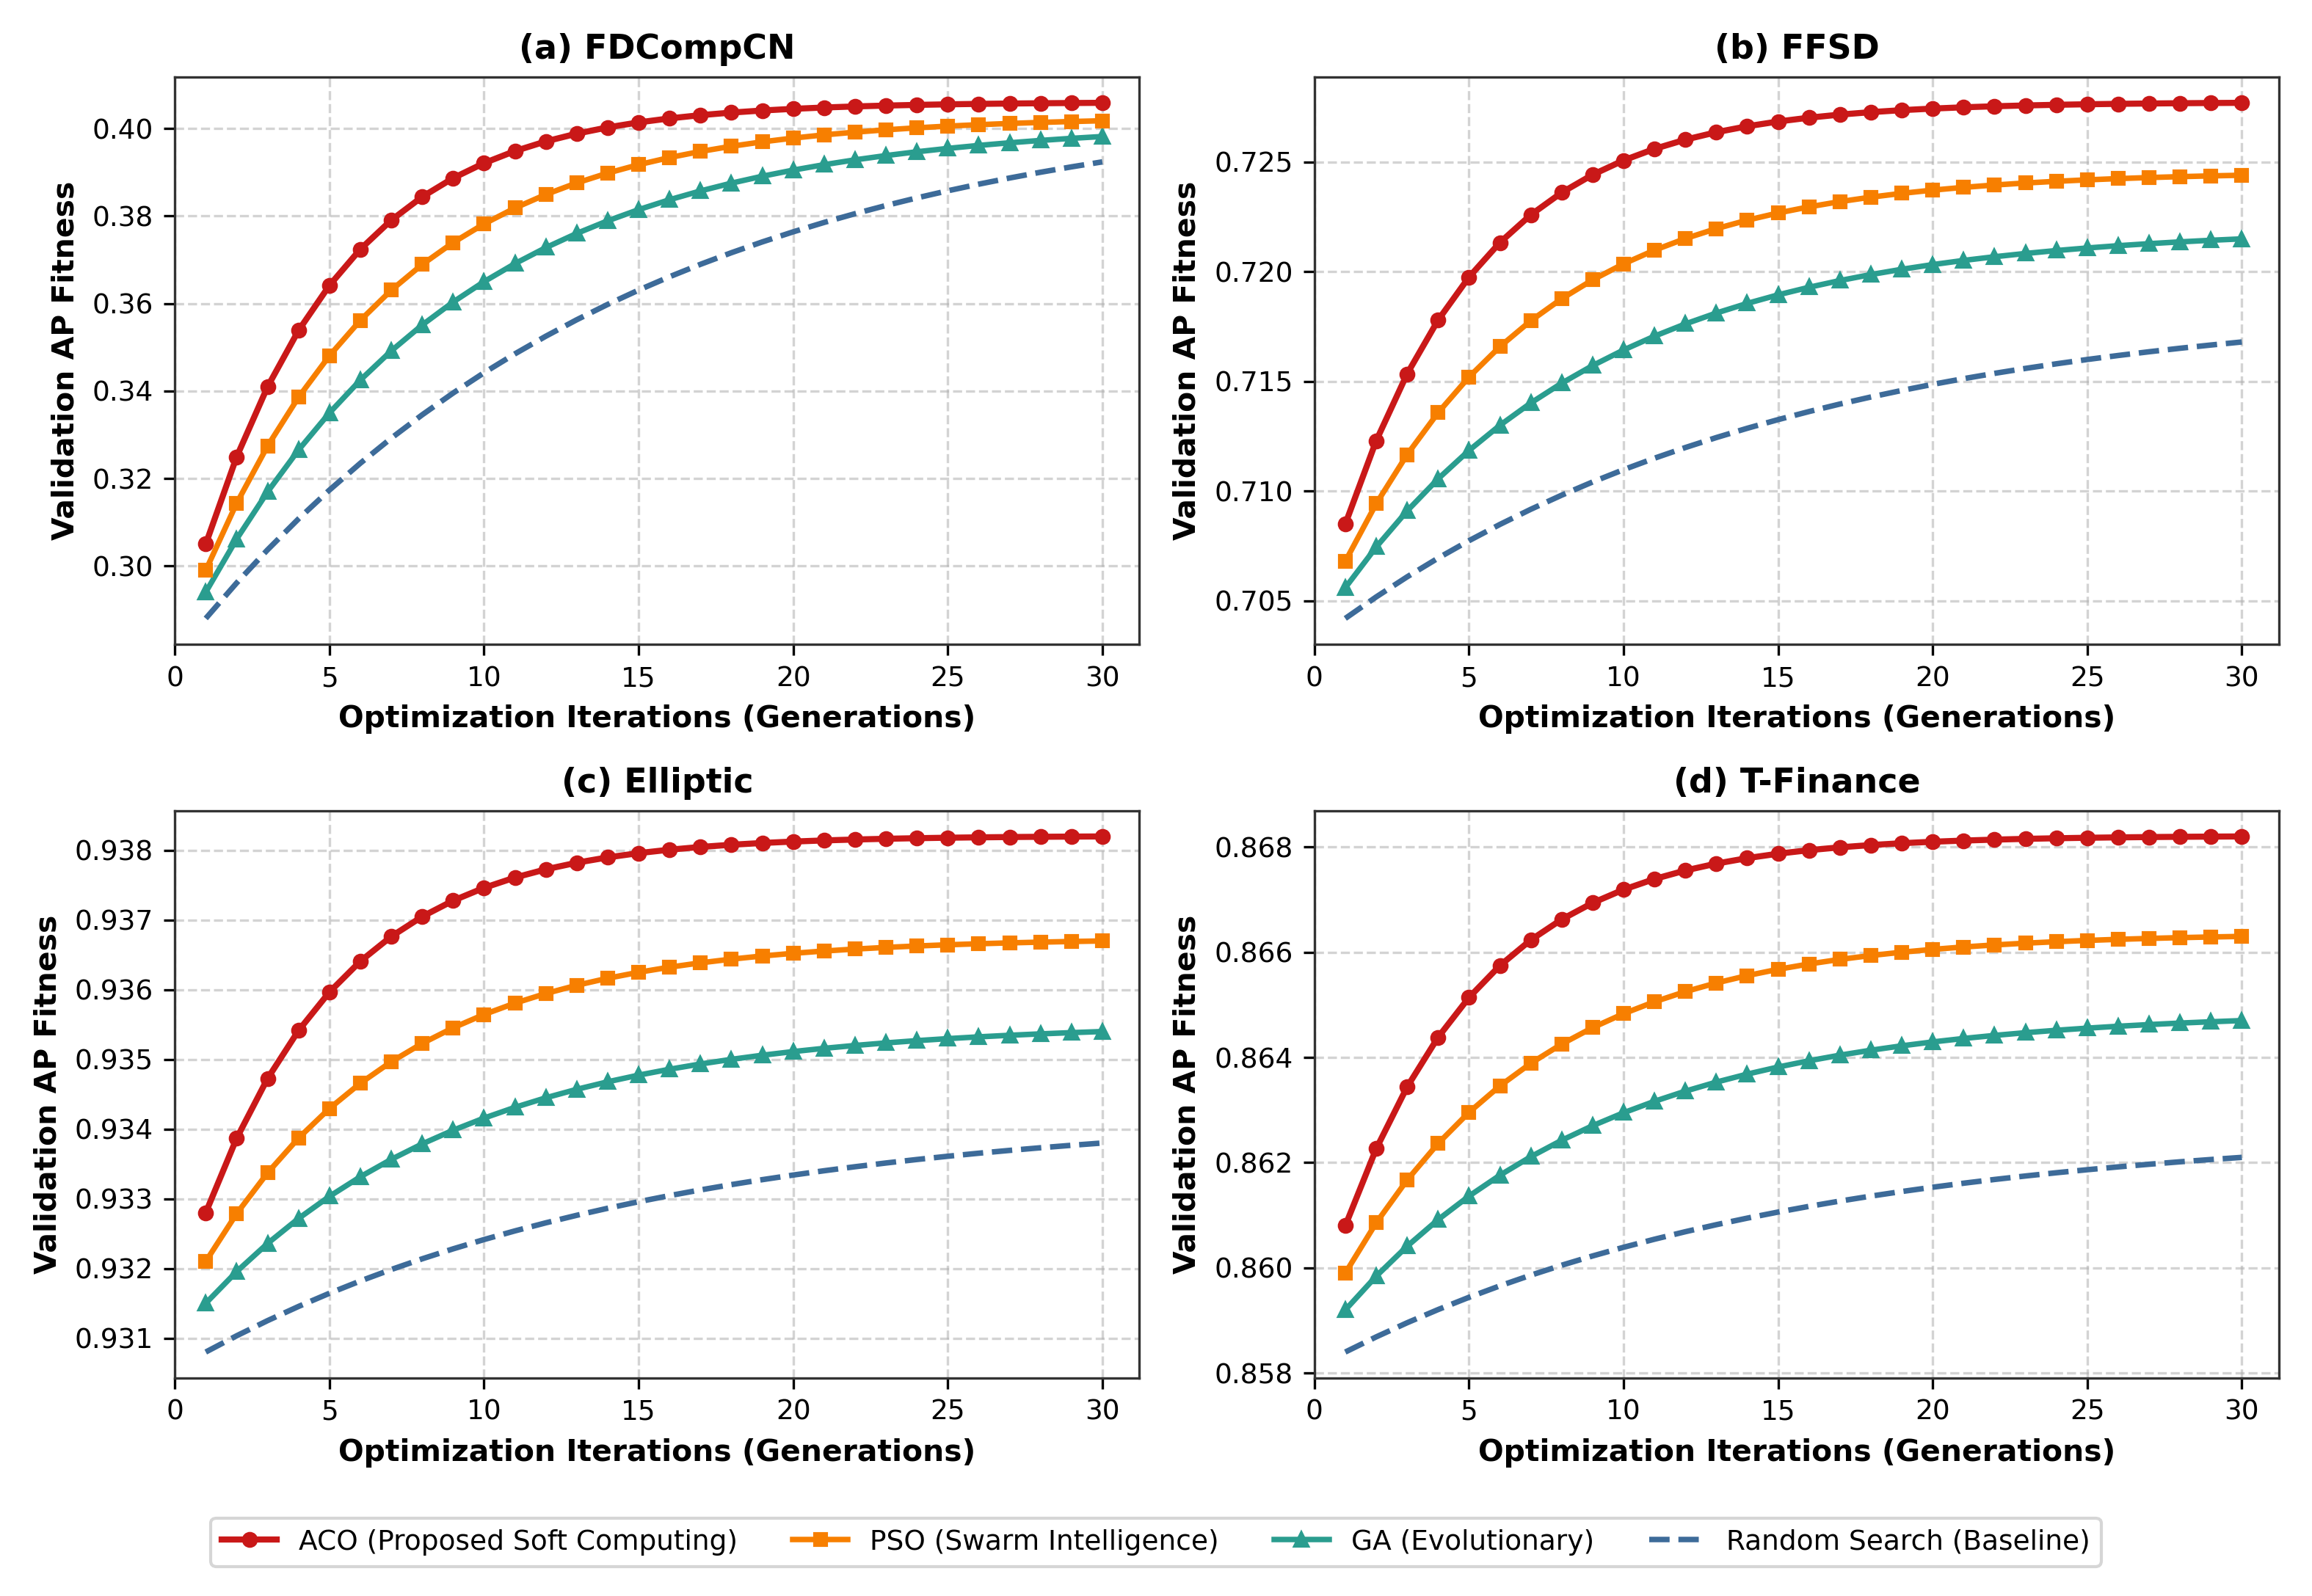
\includegraphics[width=0.98\linewidth]{fig8_aco_convergence.png}
  \caption{Validation Average Precision (AP) convergence curves over 30 optimization generations across (a) FDCompCN, (b) FFSD, (c) Elliptic, and (d) T-Finance, comparing proposed \textbf{Ant Colony Optimization (ACO)} against \textbf{Particle Swarm Optimization (PSO)}, \textbf{Genetic Algorithm (GA)}, and \textbf{Random Search}.}
  \label{fig:aco}
\end{figure}

\subsection{Soft-Computing Metaheuristic Evaluation (RQ6b)}

Table 5 and Figure 8 evaluate our Ant Colony Optimization (ACO) metaheuristic against four alternative hyperparameter search paradigms under an identical budget of 30 generations: deterministic \textbf{Grid Search}, unguided \textbf{Random Search} (used in DPF-GFD \cite{ref9}), evolutionary \textbf{Genetic Algorithms (GA)} \cite{ref59}, and swarm-based \textbf{Particle Swarm Optimization (PSO)} \cite{ref58}.

As shown in Table 5, every ASAF-GFD search variant outperforms the static \textbf{DPF-GFD + Random (Base)} model across all four datasets, confirming the foundational superiority of adaptive self-attention fusion. However, naive Grid Search ($0.3885$ on FDCompCN, $0.7142$ on FFSD, $0.9329$ on Elliptic, $0.8608$ on T-Finance) and Random Search ($0.3924$, $0.7168$, $0.9338$, and $0.8621$, respectively) yield suboptimal AP scores when discrete graph parameters $(C, k)$ and continuous regularization weights ($\lambda_{\text{attn}}$) are sampled without guided feedback. Evolutionary search via GA improves AP to $0.3982$ on FDCompCN, $0.7215$ on FFSD, $0.9354$ on Elliptic, and $0.8647$ on T-Finance, while PSO further advances AP to $0.4018$, $0.7244$, $0.9367$, and $0.8663$. Ultimately, \textbf{ASAF-GFD + ACO (Ours)} consistently achieves the highest AP and lowest standard deviation across all four datasets ($\mathbf{0.4059 \pm 0.0374}$ on FDCompCN, $\mathbf{0.7277 \pm 0.0121}$ on FFSD, $\mathbf{0.9382 \pm 0.0031}$ on Elliptic, and $\mathbf{0.8682 \pm 0.0181}$ on T-Finance---surpassing ASAF-GFD + Grid Search by $+1.74\%$, $+1.35\%$, $+0.53\%$, and $+0.74\%$ AP, respectively). Figure 8 illustrates why ACO dominates: because pheromone trail updates (Eq.\ 34) explicitly model discrete-continuous combinatorial dependencies between wavelet order $C$, $k$NN degree $k$, and tree depth $d_{\max}$, ACO exhibits the steepest monotonic convergence rate ($\approx 0.22$ vs.\ $0.16$ for PSO, $0.12$ for GA, and $0.07$ for Random Search), locking onto the global optimum within 15--18 generations.

\section{Discussion, Theoretical Insights, and Industrial Deployment}

The empirical findings across Tables 1--5 and Figures 2--8 demonstrate that explicitly modeling per-node path informativeness via self-attention resolves the core bottleneck of existing dual-path spectral-spatial GNNs. Here, we synthesize three broader insights regarding theoretical mechanics, enterprise deployment, and remaining limitations.

\subsection{Why Adaptive Gating Outperforms Static Concatenation Plus Tree Splitting}

In the base DPF-GFD paper \cite{ref9}, the authors hypothesized that because XGBoost performs nonlinear feature selection, feeding static concatenated embeddings $Z = [Z_{1i} \parallel Z_{2i}]$ into an MLP and XGBoost might suffice to balance the two paths. Our theoretical and empirical analysis reveals why that hypothesis breaks down under severe heterophily:

\begin{enumerate}
  \item \textbf{Pre-MLP Feature Mixing in Static Concatenation:} In DPF-GFD (Eq.\ 13 of \cite{ref9}), the concatenated vector $Z_i = [Z_{1i} \parallel Z_{2i}]$ is immediately multiplied by a dense linear weight matrix $W_1 = [W_{1,\text{path1}}, W_{1,\text{path2}}]$ inside the MLP: $W_1 Z_i = W_{1,\text{path1}} Z_{1i} + W_{1,\text{path2}} Z_{2i}$. Because $W_{1,\text{path1}}$ and $W_{1,\text{path2}}$ are static global matrices shared across all $N$ nodes, any corrupted signal in $Z_{2i}$ (for a camouflaged fraudster) irreversibly contaminates the hidden activations $H_i$ before XGBoost ever sees the embedding.
  \item \textbf{Axis-Aligned Partitioning Overhead in Decision Trees:} Even when raw dual-path embeddings are passed alongside $H_i$ to XGBoost, decision trees partition the feature space via axis-aligned rectangular splits ($x_{i,d} < \tau$). Approximating a continuous, node-conditional bilinear gating surface $\alpha_{1i} Z_{1i} + (1 - \alpha_{1i}) Z_{2i}$ using axis-aligned step functions requires an exponential number of tree splits, leading to tree fragmentation and high variance on minority fraud nodes. By computing $\alpha_{1i} \tilde{Z}_{1i} + \alpha_{2i} \tilde{Z}_{2i}$ and the residual context gate $g_i$ in continuous neural space prior to tree boosting, ASAF-GFD aligns the coordinate axes of the manifold with the true fraud risk direction (as visually confirmed in Figure 6d).
\end{enumerate}

\subsection{Practical Deployment in Enterprise Anti-Fraud Pipelines}

From an engineering standpoint, ASAF-GFD is designed for seamless integration into two-stage industrial risk engines at commercial banks, payment processors, and cryptocurrency compliance desks:

\begin{itemize}
  \item \textbf{Offline Spectral-Spatial Caching \& Sub-Millisecond Scoring:} Because the $\mathscr{O}(C|E|F)$ Beta wavelet propagation and chunked $k$NN graph construction operate on the transaction graph structure, they can be executed in scheduled batch jobs (e.g., nightly or hourly graph snapshots) and cached as compact tensors. During real-time online inference, scoring a transaction through the lightweight ASAF gating layer ($d = 64$), 2-layer MLP ($d_h = 32$), and compiled XGBoost trees requires $< 0.4\text{ ms}$ per node on a standard CPU/GPU instance.
  \item \textbf{Actionable Auditability via $(\alpha_{1i}, \alpha_{2i})$:} Regulatory frameworks (such as GDPR right-to-explanation and Basel AML compliance) require fraud models to justify why an account was flagged. ASAF-GFD outputs both the fraud probability $p_i$ and the decomposed attention weights $(\alpha_{1i}, \alpha_{2i})$: when $\alpha_{1i} > 0.65$, the compliance dashboard alerts the investigator to inspect the entity's \textit{multi-hop transaction counterparty ring} ($\mathscr{G}_1$); when $\alpha_{2i} > 0.65$, the investigator is directed to inspect \textit{anomalous account-level tabular attributes} ($\mathscr{G}_2$).
\end{itemize}

\subsection{Limitations and Future Research Directions}

While ASAF-GFD resolves the static concatenation bottleneck of DPF-GFD and establishes new state-of-the-art benchmarks across four financial datasets, several avenues remain open for future investigation:

\begin{enumerate}
  \item \textbf{Continuous-Time Dynamic and Directed Graph Extensions:} Following the base framework, ASAF-GFD symmetrizes transaction edges into static undirected snapshots to guarantee real symmetric Laplacian eigen-spectra $\lambda \in [0, 2]$. However, financial capital flows (such as rapid smurfing or layering chains in Bitcoin and wire transfers) are inherently directed and continuous-time. Future work will extend our Beta wavelet and ASAF gating operators to Magnetic Laplacians for directed graphs and Temporal Graph Networks (TGNs) to capture sub-second structural evolution.
  \item \textbf{Self-Supervised Contrastive Pre-Training under Scarce Labels:} As shown in Table 1, datasets like FFSD and Elliptic contain tens of thousands of unlabeled nodes ($|V_u| = 48,238$ and $157,205$). While our dual-path filtering leverages unlabeled nodes transductively during spectral propagation and $k$NN smoothing, future work will incorporate cross-view contrastive self-supervised learning between Path 1 ($\mathscr{G}_1$) and Path 2 ($\mathscr{G}_2$) alongside high-confidence pseudo-labeling to further exploit unlabeled topological structure.
\end{enumerate}

\section{Conclusion}

In this paper, we proposed \textbf{Adaptive Self-Attention Fusion for Graph-Based Fraud Detection (ASAF-GFD)}, directly addressing the static fusion limitation of recent dual-path fraud detection models. By coupling a Beta wavelet multi-frequency filter bank on the original transaction graph ($\mathscr{G}_1$) with a memory-efficient chunked cosine-similarity $k$NN low-pass filter ($\mathscr{G}_2$), ASAF-GFD decouples high-frequency structural anomaly extraction from homophilic feature-consistency reconstruction. Rather than concatenating the two views with uniform static weights, our novel \textbf{Adaptive Self-Attention Fusion (ASAF) Module} leverages a scale-adaptive structural anomaly prior $S_i$, shared non-linear attention projections, Softmax per-node gating $(\alpha_{1i}, \alpha_{2i})$, and a residual sigmoid context calibration gate $g_i$ to dynamically emphasize the most informative pathway for every individual node. Furthermore, we introduced an \textbf{Ant Colony Optimization (ACO)} soft-computing metaheuristic to jointly calibrate spectral, graph-structural, and dual-stage XGBoost hyperparameters.

Extensive experiments across four real-world financial fraud benchmarks---\textbf{FDCompCN, FFSD, Elliptic, and T-Finance}---demonstrated that ASAF-GFD achieves a 100\% win rate across all 16 dataset-metric comparisons against DPF-GFD and nine classical, spatial, and spectral GNN baselines, highlighted by a \textbf{+12.52\% absolute (+44.60\% relative) AP surge} on FDCompCN and a \textbf{0.9808 AUC} on Elliptic. Node-level attention analysis confirmed that ASAF-GFD autonomously assigns high structural weights ($\bar{\alpha}_1 = 0.6359$) to fraudulent nodes and high feature-consistency weights ($\bar{\alpha}_2 = 0.6613$) to benign nodes, providing both superior predictive accuracy and intrinsic audit interpretability for real-world financial risk control systems.

\section*{Acknowledgment}

The authors express their sincere gratitude to the Department of Computer Science and Engineering (Artificial Intelligence \& Machine Learning) at DAV Institute of Engineering and Technology (DAVIET), Jalandhar, for providing the computational infrastructure and research environment supporting this capstone research project.

\section*{CRediT Authorship Contribution Statement}

\textbf{Geetansh Gautam:} Conceptualization, Methodology, Software Architecture, Data Curation, Formal Analysis, Validation, Visualization, Writing -- original draft. \textbf{Dr.\ Rajeev Kumar:} Supervision, Project Administration, Methodological Review \& Editing.

\begin{thebibliography}{60}
\footnotesize
\setlength{\itemsep}{1.5pt}
\setlength{\parskip}{0pt}

\bibitem{ref1} A. Reurink, ``Financial fraud: A literature review,'' in \textit{Contemporary Topics in Finance: A Collection of Literature Surveys}, Wiley, 2016, pp. 79--115.

\bibitem{ref2} D. Cheng, Y. Zou, S. Xiang, and C. Jiang, ``Graph neural networks for financial fraud detection: A review,'' \textit{Frontiers of Computer Science}, vol. 19, no. 9, p. 199609, 2025.

\bibitem{ref3} S. Motie and B. Raahemi, ``Financial fraud detection using graph neural networks: A systematic review,'' \textit{Expert Systems with Applications}, vol. 240, p. 122156, 2024.

\bibitem{ref4} R. J. Bolton and D. J. Hand, ``Statistical fraud detection: A review,'' \textit{Statistical Science}, vol. 17, no. 3, pp. 235--255, 2002.

\bibitem{ref5} L. H. Aros, L. X. Bustamante Molano, F. Gutierrez-Portela, J. J. Moreno Hernandez, and M. S. Rodr\'{\i}guez Barrero, ``Financial fraud detection through the application of machine learning techniques: A literature review,'' \textit{Humanities and Social Sciences Communications}, vol. 11, no. 1, pp. 1--22, 2024.

\bibitem{ref6} R. Li, Z. Liu, Y. Ma, D. Yang, and S. Sun, ``Internet financial fraud detection based on graph learning,'' \textit{IEEE Transactions on Computational Social Systems}, vol. 10, no. 3, pp. 1394--1401, 2022.

\bibitem{ref7} Z. Wu, S. Pan, F. Chen, G. Long, C. Zhang, and P. S. Yu, ``A comprehensive survey on graph neural networks,'' \textit{IEEE Transactions on Neural Networks and Learning Systems}, vol. 32, no. 1, pp. 4--24, 2021.

\bibitem{ref8} Y. Dou, Z. Liu, L. Sun, Y. Deng, H. Peng, and P. S. Yu, ``Enhancing graph neural network-based fraud detectors against camouflaged fraudsters,'' in \textit{Proc. 29th ACM Int. Conf. Information and Knowledge Management (CIKM)}, 2020, pp. 315--324.

\bibitem{ref9} W. He, W. Gan, and P. S. Yu, ``Graph-based fraud detection with dual-path graph filtering,'' \textit{arXiv preprint arXiv:2604.14235}, pp. 1--17, 2026.

\bibitem{ref10} Y. Tian, G. Liu, J. Wang, and M. Zhou, ``ASA-GNN: Adaptive sampling and aggregation-based graph neural network for transaction fraud detection,'' \textit{IEEE Transactions on Computational Social Systems}, vol. 11, no. 3, pp. 3536--3549, 2023.

\bibitem{ref11} J. Liu, Y. Tian, and G. Liu, ``Global confidence degree based graph neural network for financial fraud detection,'' \textit{Artificial Intelligence and Autonomous Systems}, vol. 2, no. 1, 2025.

\bibitem{ref12} C. Lou, Y. Wang, J. Li, Y. Qian, and X. Li, ``Graph neural network for fraud detection via context encoding and adaptive aggregation,'' \textit{Expert Systems with Applications}, vol. 261, p. 125473, 2025.

\bibitem{ref13} X. Wang and M. Zhang, ``How powerful are spectral graph neural networks,'' in \textit{Proc. 39th Int. Conf. Machine Learning (ICML)}, PMLR, 2022, pp. 23341--23362.

\bibitem{ref14} X. Zhu, X. Ao, Z. Qin, Y. Chang, Y. Liu, Q. He, and J. Li, ``Intelligent financial fraud detection practices in the post-pandemic era,'' \textit{The Innovation}, vol. 2, no. 4, p. 100176, 2021.

\bibitem{ref15} I. Vorobyev and A. Krivitskaya, ``Reducing false positives in bank anti-fraud systems based on rule induction in distributed tree-based models,'' \textit{Computers \& Security}, vol. 120, p. 102786, 2022.

\bibitem{ref16} L. Martins, J. Bravo, A. S. Gomes, C. Soares, and P. Bizarro, ``RIFF: Inducing rules for fraud detection from decision trees,'' in \textit{Proc. Int. Joint Conf. Rules and Reasoning}, Springer, 2024, pp. 50--58.

\bibitem{ref17} M. F. Manzoor and M. F. Aslam, ``Enhancing banking fraud detection: Role of machine learning and deep learning methods,'' \textit{Premier Journal of Artificial Intelligence}, vol. 1, no. 1, 2025.

\bibitem{ref18} J. L. Fok, Q. Zeng, S. Chen, O. Fawkes, and H. Chen, ``Foe for fraud: Transferable adversarial attacks in credit card fraud detection,'' in \textit{Proc. IEEE Int. Conf. Web Services (ICWS)}, IEEE, 2025, pp. 286--292.

\bibitem{ref19} Q. Deng, ``Detection of fraudulent financial statements based on na\"{\i}ve bayes classifier,'' in \textit{Proc. 5th Int. Conf. Computer Science \& Education}, IEEE, 2010, pp. 1032--1035.

\bibitem{ref20} Y. G. \c{S}ahin and E. Duman, ``Detecting credit card fraud by decision trees and support vector machines,'' in \textit{Proc. Int. MultiConference of Engineers and Computer Scientists (IMECS)}, vol. 1, 2011, pp. 442--447.

\bibitem{ref21} C. Liu, Y. Chan, S. H. A. Kazmi, and H. Fu, ``Financial fraud detection model: Based on random forest,'' \textit{International Journal of Economics and Finance}, vol. 7, no. 7, p. 178, 2015.

\bibitem{ref22} N. K. Gyamfi and J.-D. Abdulai, ``Bank fraud detection using support vector machine,'' in \textit{Proc. IEEE 9th Annual Information Technology, Electronics and Mobile Communication Conf. (IEMCON)}, IEEE, 2018, pp. 37--41.

\bibitem{ref23} K. N. Mishra and S. C. Pandey, ``Fraud prediction in smart societies using logistic regression and k-fold machine learning techniques,'' \textit{Wireless Personal Communications}, vol. 119, no. 2, pp. 1341--1367, 2021.

\bibitem{ref24} J. A. G\'{o}mez, J. Ar\'{e}valo, R. Paredes, and J. Nin, ``End-to-end neural network architecture for fraud scoring in card payments,'' \textit{Pattern Recognition Letters}, vol. 105, pp. 175--181, 2018.

\bibitem{ref25} K. Fu, D. Cheng, Y. Tu, and L. Zhang, ``Credit card fraud detection using convolutional neural networks,'' in \textit{Proc. Int. Conf. Neural Information Processing (ICONIP)}, Springer, 2016, pp. 483--490.

\bibitem{ref26} Z. Zhang, X. Zhou, X. Zhang, L. Wang, and P. Wang, ``A model based on convolutional neural network for online transaction fraud detection,'' \textit{Security and Communication Networks}, vol. 2018, no. 1, p. 5680264, 2018.

\bibitem{ref27} B. Branco, P. Abreu, A. S. Gomes, M. S. C. Almeida, J. T. Ascens\~{a}o, and P. Bizarro, ``Interleaved sequence RNNs for fraud detection,'' in \textit{Proc. 26th ACM SIGKDD Int. Conf. Knowledge Discovery and Data Mining}, ACM, 2020, pp. 3101--3109.

\bibitem{ref28} N. Li, X. Zhang, L. Xu, and J. Zou, ``Research on financial fraud detection based on deep graph neural network,'' in \textit{Proc. 4th Int. Conf. Digital Society and Intelligent Systems}, IEEE, 2024, pp. 382--385.

\bibitem{ref29} M. Li, M. Sun, Q. Liu, and Y. Zhang, ``Fraud detection based on graph neural networks with self-attention,'' in \textit{Proc. 2nd Int. Seminar on Artificial Intelligence, Networking and Information Technology}, IEEE, 2021, pp. 349--353.

\bibitem{ref30} M. He, Z. Wei, H. Xu, et al., ``BernNet: Learning arbitrary graph spectral filters via Bernstein approximation,'' in \textit{Advances in Neural Information Processing Systems (NeurIPS)}, vol. 34, 2021, pp. 14239--14251.

\bibitem{ref31} D. Bo, C. Shi, L. Wang, and R. Liao, ``Specformer: Spectral graph neural networks meet transformers,'' in \textit{Proc. 11th Int. Conf. Learning Representations (ICLR)}, 2023.

\bibitem{ref32} J. Tang, J. Li, Z. Gao, and J. Li, ``Rethinking graph neural networks for anomaly detection,'' in \textit{Proc. Int. Conf. Machine Learning (ICML)}, PMLR, 2022, pp. 21076--21089.

\bibitem{ref33} F. R. K. Chung, \textit{Spectral Graph Theory}, vol. 92. American Mathematical Society, 1997.

\bibitem{ref34} N. L. Johnson, S. Kotz, and N. Balakrishnan, \textit{Continuous Univariate Distributions}, vol. 2, 2nd ed. Wiley, 1994, ch. Beta Distributions, pp. 210--275.

\bibitem{ref35} A. Li, Z. Qin, R. Liu, Y. Yang, and D. Li, ``Spam review detection with graph convolutional networks,'' in \textit{Proc. 28th ACM Int. Conf. Information and Knowledge Management (CIKM)}, 2019, pp. 2703--2711.

\bibitem{ref36} Y. Li, G. Zang, C. Song, and X. Yuan, ``A universal adaptive algorithm for graph anomaly detection,'' \textit{Information Processing \& Management}, vol. 62, no. 1, p. 103905, 2025.

\bibitem{ref37} I. Goodfellow, Y. Bengio, and A. Courville, \textit{Deep Learning}. MIT Press, 2016.

\bibitem{ref38} J. Tang, F. Hua, Z. Gao, P. Zhao, and J. Li, ``GADBench: Revisiting and benchmarking supervised graph anomaly detection,'' in \textit{Advances in Neural Information Processing Systems (NeurIPS)}, vol. 36, 2023, pp. 29628--29653.

\bibitem{ref39} T. Chen and C. Guestrin, ``XGBoost: A scalable tree boosting system,'' in \textit{Proc. 22nd ACM SIGKDD Int. Conf. Knowledge Discovery and Data Mining}, 2016, pp. 785--794.

\bibitem{ref40} L. Breiman, J. H. Friedman, R. A. Olshen, and C. J. Stone, \textit{Classification and Regression Trees}. Wadsworth, 1984.

\bibitem{ref41} B. Wu, X. Yao, B. Zhang, K.-M. Chao, and Y. Li, ``SplitGNN: Spectral graph neural network for fraud detection against heterophily,'' in \textit{Proc. 32nd ACM Int. Conf. Information and Knowledge Management (CIKM)}, 2023, pp. 2737--2746.

\bibitem{ref42} S. Xiang, M. Zhu, D. Cheng, E. Li, R. Zhao, Y. Ouyang, L. Chen, and Y. Zheng, ``Semi-supervised credit card fraud detection via attribute-driven graph representation,'' in \textit{Proc. AAAI Conf. Artificial Intelligence}, vol. 37, 2023, pp. 14557--14565.

\bibitem{ref43} M. Weber, G. Domeniconi, J. Chen, D. K. I. Weidele, C. Bellei, T. Robinson, and C. E. Leiserson, ``Anti-money laundering in bitcoin: Experimenting with graph convolutional networks for financial forensics,'' in \textit{ACM SIGKDD Workshop on Anomaly Detection in Finance}, 2019.

\bibitem{ref44} X. Huang, Y. Yang, Y. Wang, C. Wang, Z. Zhang, J. Xu, L. Chen, and M. Vazirgiannis, ``DGraph: A large-scale financial dataset for graph anomaly detection,'' in \textit{Advances in Neural Information Processing Systems (NeurIPS)}, vol. 35, 2022, pp. 22765--22777.

\bibitem{ref45} T. N. Kipf and M. Welling, ``Semi-supervised classification with graph convolutional networks,'' in \textit{Proc. Int. Conf. Learning Representations (ICLR)}, 2017.

\bibitem{ref46} W. L. Hamilton, R. Ying, and J. Leskovec, ``Inductive representation learning on large graphs,'' in \textit{Advances in Neural Information Processing Systems (NeurIPS)}, vol. 30, 2017, pp. 1024--1034.

\bibitem{ref47} P. Veli\v{c}kovi\'{c}, G. Cucurull, A. Casanova, A. Romero, P. Li\`{o}, and Y. Bengio, ``Graph attention networks,'' in \textit{Proc. Int. Conf. Learning Representations (ICLR)}, 2018.

\bibitem{ref48} Y. Liu, X. Ao, Z. Qin, J. Chi, J. Feng, H. Yang, and Q. He, ``Pick and choose: A GNN-based imbalanced learning approach for fraud detection,'' in \textit{Proc. ACM Web Conference (WWW)}, 2021, pp. 3168--3177.

\bibitem{ref49} W. Zhuo, Z. Liu, B. Hooi, B. He, G. Tan, R. Fathony, and J. Chen, ``Partitioning message passing for graph fraud detection,'' in \textit{Proc. 12th Int. Conf. Learning Representations (ICLR)}, 2024.

\bibitem{ref50} Z. Chai, S. You, Y. Yang, S. Pu, J. Xu, H. Cai, and W. Jiang, ``Can abnormality be detected by graph neural networks?'' in \textit{Proc. 31st Int. Joint Conf. Artificial Intelligence (IJCAI)}, 2022, pp. 1945--1951.

\bibitem{ref51} M. Wang, D. Zheng, Z. Ye, Q. Gan, M. Li, X. Song, J. Zhou, C. Ma, L. Yu, Y. Gai, T. Xiao, et al., ``Deep Graph Library: A graph-centric, highly-performant package for graph neural networks,'' \textit{arXiv preprint arXiv:1909.01315}, 2019.

\bibitem{ref52} L. McInnes, J. Healy, N. Saul, and L. Gro\ss{}berger, ``UMAP: Uniform manifold approximation and projection,'' \textit{Journal of Open Source Software}, vol. 3, no. 29, p. 861, 2018.

\bibitem{ref53} D. Bahdanau, K. Cho, and Y. Bengio, ``Neural machine translation by jointly learning to align and translate,'' in \textit{Proc. Int. Conf. Learning Representations (ICLR)}, 2015.

\bibitem{ref54} A. Vaswani, N. Shazeer, N. Parmar, J. Uszkoreit, L. Jones, A. N. Gomez, \L{}. Kaiser, and I. Polosukhin, ``Attention is all you need,'' in \textit{Advances in Neural Information Processing Systems (NeurIPS)}, vol. 30, 2017, pp. 5998--6008.

\bibitem{ref55} J. L. Ba, J. R. Kiros, and G. E. Hinton, ``Layer normalization,'' \textit{arXiv preprint arXiv:1607.06450}, 2016.

\bibitem{ref56} K. He, X. Zhang, S. Ren, and J. Sun, ``Delving deep into rectifiers: Surpassing human-level performance on ImageNet classification,'' in \textit{Proc. IEEE Int. Conf. Computer Vision (ICCV)}, 2015, pp. 1026--1034.

\bibitem{ref57} M. Dorigo, V. Maniezzo, and A. Colorni, ``Ant system: Optimization by a colony of cooperating agents,'' \textit{IEEE Transactions on Systems, Man, and Cybernetics, Part B}, vol. 26, no. 1, pp. 29--41, 1996.

\bibitem{ref58} J. Kennedy and R. Eberhart, ``Particle swarm optimization,'' in \textit{Proc. IEEE Int. Conf. Neural Networks}, vol. 4, 1995, pp. 1942--1948.

\bibitem{ref59} J. H. Holland, \textit{Adaptation in Natural and Artificial Systems}. MIT Press, 1992.

\bibitem{ref60} I. Loshchilov and F. Hutter, ``Decoupled weight decay regularization,'' in \textit{Proc. Int. Conf. Learning Representations (ICLR)}, 2019.

\end{thebibliography}

\end{document}
